%%% pour la compilation en local 
%%% !TeX program = XeLaTeX
%%% !TeX options = -shell-escape
%%% !BIB program = biber

\documentclass[11pt,a4paper]{article}

% --- GESTION DE LA LANGUE ET DES POLICES (XELATEX) ---
\usepackage{fontspec}           % Indispensable pour XeLaTeX pour charger les polices système
\usepackage[french]{babel}      % Support de la langue française

% --- Définition des polices (à adapter) ---
\setmonofont{DejaVu Sans Mono}  % Police pour le code,
% --- GESTION DE LA GÉOMÉTRIE ET MISE EN PAGE ---
\usepackage{geometry}
\geometry{a4paper, margin=1.5cm, bottom=1.5cm} % Une seule déclaration suffit, la dernière est prise en compte

% --- PAQUETS POUR LES MATHS ---
\usepackage{amsmath}
\usepackage{amsfonts}
\usepackage{amssymb}

% --- PAQUETS GRAPHIQUES ET COULEURS ---
\usepackage{graphicx}           % Inclusion d'images
\usepackage{xcolor}             % Gestion des couleurs
\usepackage{tikz}               % Pour les schémas
\usetikzlibrary{shapes.geometric, arrows, positioning, automata, arrows.meta, fit, calc, backgrounds}
\usepackage{adjustbox}          % Pour ajuster des boîtes 
\graphicspath{ {figures/} }
\usepackage{array}

% Définition des styles pour les nœuds BPMN/Flowchart
\usepackage{pdflscape} 
\tikzset{
    % Style pour les événements (début/fin)
    event/.style={circle, draw, fill=green!20, minimum size=1.0cm, text width=1.8cm, text centered},
    % Style pour les tâches/processus
    task/.style={rectangle, draw, fill=blue!20, rounded corners, minimum height=1.0cm, minimum width=2.2cm, text width=2.8cm, text centered},
    % Style pour les données/artefacts échangés
    data/.style={trapezium, trapezium left angle=70, trapezium right angle=110, draw, fill=yellow!20, minimum height=0.8cm, text width=2.5cm, text centered, inner xsep=0pt},
    % Style pour les passerelles/décisions (non utilisé ici)
    gateway/.style={diamond, draw, fill=orange!20, aspect=1.5, inner sep=0pt},
    % Style pour les flèches de séquence
    seq/.style={-Latex, thick},
    % Style pour les flèches de message (communication entre couloirs)
    msg/.style={-Latex, thick, dashed}
}

% --- MISE EN FORME DU TEXTE ET TABLEAUX ---
\usepackage{enumitem}   % Pour personnaliser les listes
\setlist[itemize,1]{label=\textbullet}
\setlist[itemize,2]{label=-}
\usepackage{ulem}   % Pour barrer du texte (\sout)
\usepackage{longtable}
\usepackage{tabularx,booktabs}
\usepackage{float}
\usepackage{pifont} % pour styliser les bullets
\usepackage{caption}

% --- MISE EN FORME DU CODE (MINTED) ---
\usepackage[outputdir=build]{minted}

\usepackage{csquotes} % Gestion avancée des guillemets (A CHARGER APRES MINTED)

\usepackage[backend=biber,style=apa,sorting=none]{biblatex}
\DeclareLanguageMapping{french}{french-apa}
\addbibresource{ref.bib}
\let\cite\parencite

% --- LIENS HYPERTEXTE ET COULEURS PERSONNALISÉES ---
\usepackage{hyperref}
\definecolor{darkgreen}{rgb}{0.0, 0.5, 0.0}
\definecolor{darkblue}{rgb}{0.0, 0.0, 0.5}
\definecolor{darkred}{rgb}{0.5, 0.0, 0.0}
\hypersetup{
    colorlinks=true,
    linkcolor=blue,
    filecolor=magenta,      
    urlcolor=cyan,
    citecolor=blue
}

% --- COMMANDES PERSONNALISÉES ---
\definecolor{lightgray}{rgb}{0.92, 0.92, 0.92}
\newcommand{\code}[1]{\colorbox{lightgray}{\texttt{\small #1}}}
\newcommand{\var}[1]{\textit{#1}}
\newcommand{\vartype}[1]{\textcolor{darkgreen}{#1}}
\newcommand{\methodname}[1]{\textbf{\textcolor{darkblue}{#1}}}
\newcommand{\param}[1]{\code{#1}}
\newcommand{\rettype}[1]{\textcolor{darkred}{#1}}
\newcommand{\jsfunc}[1]{\textcolor{purple}{\textit{#1}}} 
\newcommand{\filepath}[1]{\textit{#1}}

\let\labelitemi\labelitemii

% --- INFORMATIONS DU DOCUMENT ---
\title{\textbf{Conception et implémentation d'un exerciseur automatique pour l'enseignement de la programmation}}
\author{Julien Mateesco}
%footnote 'sous la direction de', juré expert
\date{8 sept. 2025}

\begin{document}
\maketitle

\begin{abstract}
Ce rapport présentera un outil-auteur et sa réalisation, faite dans le cadre du programme de formation GymInf, répondant à la question ``comment soutenir l'apprentissage par la méthode PRIMM de la programmation Python chez les débutants, avec visualisation logigrammme''. L'outil existe, visible sous \url{https://github.com/edu-mateescoj/gyminf} et propose principalement quatre fonctionnalités :
\begin{itemize}
    \item[\ding{51}] un générateur automatique (infini) de code Python valide (syntaxiquement correct, qui s'exécute dans l'environnement Pyodide et qui termine) et de niveau pédagogique adapté aux besoins définis par l'utilisateur, exécuté dans le navigateur \textit{full front-end}.
    \item[\ding{51}] un traducteur de code Python en logigramme, exécuté et affiché dans le navigateur \textit{full front-end}, et modifiable par l'utilisateur.
    \item[\ding{51}] le questionnement des élèves sur les valeurs des variables à l'issue du code proposé, avec la rétroaction réussite/échec correspondante, ainsi qu'une simulation de console d'exécution, dans le navigateur \textit{full front-end}.
    \item[\ding{51}] la constitution sur serveur d'une base de données enregistrant les codes Python générés et les interactions élèves correspondantes, laissant la possibilité de suivre individuellement l'évolution des élèves dans leurs interactions avec les codes proposés.
\end{itemize}   
Nous présenterons d'abord les contextes qui ont présidé à la réalisation de cet outil prévu pour être utilisé en classe à très brève échéance, ainsi que son architecture logique. Nous alternerons donc entre les côtés technique et fonctionnel. Le travail de développement informatique prenant une coloration didactique, nous donnerons une description logicielle de l'ensemble, ne fournissant des détails d'implémentation que sur les contributions essentielles que sont: \begin{enumerate}
    \item le générateur Javascript de codes Python tournant dans le navigateur, aléatoires mais contrôlables et de niveau pédagogique
    \item le traducteur Javascript de code Python en graphique logigramme rendu dans le navigateur par Mermaid
    \item le serveur Flask (Python) enregistrant les interactions élèves face aux codes proposés pour construire une base de données didactiques. 
\end{enumerate} 
Le présent rapport n'a pas vocation à être un mode d'emploi ou une documentation technique exhaustive, mais une explication des fonctionnalités implémentées et des choix qui ont été faits.
\end{abstract}

\clearpage
\tableofcontents
\listoffigures

\clearpage
\section{Introduction}
\subsection{Préambule philosophique}
Notre projet a été construit à une époque marquée simultanément par trois phénomènes apparemment contradictoires : 
\begin{itemize} 
    \item la massification de l'apprentissage de la programmation, aujourd'hui proposée à \textbf{tous les élèves de filière secondaire académique} (gymnasiale, générale) 
    \item une \textbf{disparition annoncée de la pratique de l'écriture humaine de code} informatique, ce qui questionne la possible disparition de l'écriture de code comme compétence socialement valorisée
    \item l'ubiquité du \textbf{numérique dans la vie quotidienne}, en particulier pour les actuels élèves du secondaire, nés après l'avènement du smartphone et du Web 2.0 
\end{itemize}
Il nous semble donc d'autant plus urgent de proposer des \textit{outils conviviaux} susceptibles de redonner aux futurs citoyens une capacité d'agir dans notre monde numérique. Nous empruntons ici l'expression d'Ivan Illich \cite{Illich} pour qui des ``outils conviviaux'' sont le contraire de l'outil ``dominant'' (exemple aujourd'hui: l'algorithme qui décide pour nous, à notre insu). Sont ``conviviales'' les techniques autolimitées, compréhensibles et modifiables par leurs usagers, que chacun peut utiliser, réparer et adapter sans dépendre d’experts ni d’institutions, afin d’accroître l’autonomie et la coopération plutôt que la dépendance aux systèmes.
\`{A} l'époque contemporaine, Shoshana Zuboff décrit notre ``capitalisme de surveillance'' - aux antipodes de la convivialité d’Illich - où l’outil capture les comportements plutôt que d’étendre la capacité d’agir.
Les deux autres concepts qui nous semblent essentiels pour essayer de penser la valeur sociale d'un nouveau service numérique sont : le ``Panoptique'' \cite{Foucault} de Michel Foucault (métaphore d’un pouvoir disciplinaire fondé sur la visibilité asymétrique) et la ``Société de contrôle'' \cite{Deleuze} de Gilles Deleuze (très proche des logiques de plateformes et de scoring algorithmique d'aujourd'hui, des décennies après sa mort).
L’outil ``convivial'' est ainsi un critère normatif contre ces logiques panoptiques et ``contrôlantes'' : gouvernance par les usagers, transparence et autolimitation vs. extraction des données, opacité et dépendance. 
Je milite pour une évaluation critique des services numériques que nous faisons utiliser aux élèves, avec comme objectif de favoriser l’appropriation collective (Illich) et d'identifier là où elles se trouvent les logiques de surveillance et de contrôle diffus (Foucault/Deleuze).

\subsubsection{Position de principe sur l'IA générative comme outil dans les mains des élèves}
Il apparaît naturel pour beaucoup de gens aujourd'hui de déléguer aux LLM des tâches d'enseignants tant les modèles et leurs interfaces sont devenus qualitativement et quantitativement performants. On peut en effet noter à la fois la qualité des réponses proposées, instructives pour nos élèves, et d'un point de vue quantitatif l'infrastructure qui nous sert ces modèles autorise un passage à l'échelle permettant une productivité face aux élèves littéralement inhumaine, leur ubiquité soulignant la rareté et la singularité de l'interaction pédagogique enseignant - apprenant. 
De façon générale, plusieurs raisons de refuser d'inciter les élèves à utiliser massivement l'IA générative peuvent être mises en avant: \begin{enumerate}
        \item l'impact écologique (climat et environnement: énergie, eau et terres rares, etc.), 
        \item l'inadéquation par rapport à une démarche scientifique "explicative et contrôlée", 
        \item les dérives sociales des géants du numérique (non respect des normes de traitement des humains engagés dans l’entraînement des modèles),
        \item la cannibalisation des communs numériques pour l’entraînement des LLM privés (appropriation de biens publics pour la constitution de profits privés, non respect des bonnes pratiques de crawlers web pour alimenter les modèles),
    \end{enumerate}
Maintenant dans une perspective d'\textit{empowerment}, telle que les fournisseurs d'IA nous le promettent \cite{email}, une précision nous semble importante : déléguer l'interaction maître-élève à une machine et déléguer l'observation et la ``compréhension'' de l'erreur élève à une machine prive l'enseignant de la possibilité de développer son expertise didactique
 Plus spécifiquement, pour notre cas d'usage qui est la génération aléatoire d'exercices par les élèves, adapté aux besoins pédagogiques, une solution acceptable par principe aurait été la distillation d'un gros modèle produit dans des conditions \textit{fair-trade}, assez frugale pour tourner sur un serveur interne à l'école, mais c'est un autre sujet qui ne rentre pas dans le cadre de ce travail. \\ Mettre dans les mains des élèves un outil basé sur l'API d'un modèle commercial, performant mais en voie de monétisation, reste inconcevable tant cela enfreindrait mes principes que je viens de mentionner ci-dessus, en exposant les élèves au risque d'être instrumentalisés dans le processus de monétisation des IA génératives.
 
\par Les ambitions qui ont guidé mon projet se situent:
\begin{itemize}
    \item \textbf{Chez les élèves} : en leur proposant une traduction de la syntaxe textuelle Python en une syntaxe graphique logigramme, en les exerçant à la traduction d'une syntaxe à l'autre comme un entraînement; en les invitant à se faire une image mentale de la sémantique associée pour tracer la valeur des variables. Ces savoirs syntaxiques et conceptuels sont les premières étapes à mobiliser pour la résolution de nouveaux problèmes. Nous formulons donc l'espoir que notre outil contribuera au développement de leurs compétences stratégiques.
    \item \textbf{Pour la relation enseignants - apprenants}, en mettant à libre disposition un outil-auteur adaptable et capable de proposer des codes prédéfinis par l'enseignant doublé d'un système de journalisation des interactions élèves qui a le potentiel de permettre à l'enseignant un suivi très fin des élèves pour pouvoir apporter une rétroaction différenciée jusqu'au niveau individuel.
    \item \textbf{Chez les enseignants} : en proposant à la communauté enseignante un outil évolutif, nous cherchons à inviter les collègues à la collaboration pour améliorer le projet, et à l'échange sur leurs pratiques. Nous nous situons dans l'esprit de la constitution d'une ``communauté de pratique'' \cite{wenger} \item \textbf{Chez les enseignants} : en refusant de déléguer la rétroaction élève à un LLM d'IA générative et en donnant les moyens aux enseignants d'évaluer immédiatement et à long terme l'efficacité de leur action enseignante, notre espoir est de donner les moyens de développer une expertise didactique à des experts informatiques qui s'adressent maintenant à des apprenants culturellement très éloignés.
\end{itemize}
Maintenant que nous avons défini le cadre social, voyons tout d'abord d'où vient le projet, en alternant les points de vue : professionnel, personnel, pédagogique et pratique.

\subsection{Éléments de contexte}
Notre démarche tire son essence dans un but : aider les enseignants chargés de faire découvrir la programmation textuelle à des élèves débutants et culturellement aux antipodes. Situons donc ici le public cible et l'environnement concerné afin de justifier les objectifs poursuivis dans la création de notre outil. 

\subsubsection{Contexte institutionnel}
\begin{description}
    \item[Institutionnel et pédagogique:] École secondaire genevoise; enseignement de l'informatique comme discipline obligatoire pour tous les élèves de 1ère et 2ème année, mais avec très peu d’heures hebdomadaires pour chaque élève (respectivement 2 périodes et 1 seule) et dont la note ne sera pas reprise sur le diplôme de maturité: massification des effectifs d’élèves pour l’enseignant, difficulté voire opposition de certains élèves face à la programmation.
    \item[Professionnel et personnel:] Ce projet rentre dans le cadre de la validation de ma formation GymInf et doit se terminer durant le semestre académique courant.
    \item[Professionnel et institutionnel:]
    
        \begin{itemize}
        \item Constat de l'absence d’une culture de groupe de discipline, besoin de créer une “communauté de pratique”; 
        \item Très grand nombre d'élèves pour chaque enseignant. Et donc besoin de rationaliser au maximum la pratique en créant des outils automatiques, besoin d’autonomiser les élèves dans leurs apprentissages; 
        \item Indisponibilité (technique ou budgétaire) ou inadéquation des outils existants (curriculum différent, objectifs "venus d'en haut" et nécessité de se conformer à une épreuve commune)
        \end{itemize}
\end{description}
Le calendrier scolaire est rythmé par le curriculum et l'évaluation certificative qui y est attachée, aussi le développement de l'outil et le présent rapport se sont trouvé désynchronisés, ce qui explique qu'il n'y a pas eu d'analyse de l'efficacité d'un dispositif basé sur l'outil.
    
\subsubsection{Contexte didactique: surtout des hypothèses appuyées par la littérature}
\begin{enumerate}
    \item Hypothèse fondatrice, appuyée par la littérature : la pertinence de la méthodologie PRIMM \cite{Sentance2017WiPSCE} dans le cadre de l'enseignement de la programmation en particulier en école secondaire avec des classes hétérogènes \cite{Sentance2019CSE}, que nous étendons par hypothèse aux syntaxes graphiques de type logigramme. Les mêmes auteurs relèvent l'attrait de cette approche pour les enseignants, qui a priori justifie qu'on cherche à les aider dans cette approche si elle a du succès chez eux !
    \item Hypothèse forte appuyée par la littérature: les intérêts multiples d'un générateur d'exercices aléatoires \cite{messer2023}, pour autant que  l'aléa réponde à des critères pédagogiques fixés et contrôlables par l'enseignant et/ou par l'apprenant. Citons notamment comme intérêt la grande variété des questions, qui évite la mémorisation de la solution sans investissement personnel, évitant ainsi le \textit{plagiat de solutions}; le contrôle de la difficulté peut permettre une différenciation (par adaptation au niveau réel ou supposé de l'élève).
    \item Hypothèse : intérêt de la représentation logigramme (\textit{flowchart}) comme moyen d'apprentissage \cite{zimmermann2024}, et en particulier de la programmation \cite{CrewsZielger98} - en plus d'être un objectif d'apprentissage qui se justifie eu égard au contexte institutionnel.
    \item Hypothèse : intérêt de proposer des exercices de lecture de programmes textuels et graphiques avant ceux d'écriture, en référence aux taxonomies d’Anderson \& Krathwohl \cite{AndersonKrathwohl2001} et plus spécifiquement \cite{Fuller2007} pour l'enseignement de la programmation. Ces taxonomies ont en commun de placer ``comprendre'' à un niveau cognitif plus bas que ``appliquer''“comprendre” est censé être de niveau cognitif plus bas que “appliquer” ou encore “créer”. ou encore ``créer''.
    \item Hypothèse : l'intérêt d'une évaluation formative immédiate pour tester la compréhension et l'intérêt de la possibilité laissée à l'apprenant de modifier les codes proposés - textuel et logigramme - citons notamment \cite{HattieTimperley2007} et \cite{Shute2008}.
\end{enumerate}


\subsection{Objectifs fonctionnels}
Nos objectifs fonctionnels apparaissent comme des conclusions de la section précédente : nous voulons un outil qui aide les enseignants à proposer des exercices de niveau débutant en accord avec les étapes ``Predict Run Investigate Modify'' de la célèbre approche PRIMM.

\subsubsection{Besoin d'un générateur de code et de questions pertinentes}

Au niveau débutant, les classes sont hétérogènes. Nous visons donc des \emph{exercices de lecture de code} fondés sur la taxonomie des tâches au premier échelon, de difficulté \emph{ajustable} pour différencier au sein du groupe et accompagner sa progression. L’outil doit aussi \emph{décharger l’enseignant} avec : une génération automatique,un déploiement simple, un contrôle fin des paramètres.
\\
Du côté de l’élève (dimension ``Predict''), il faut recevoir programmatiquement un script Python, l’afficher dans une fenêtre avec \emph{coloration syntaxique} et \emph{numérotation des lignes}, afin de soutenir la lecture analytique. L’aléa doit être \emph{contrôlé} pour garantir une plus-value pédagogique: on \emph{choisit} explicitement les constructions à inclure dans le script, on \emph{règle} des variables didactiques (nombre de variables, domaine de valeurs, longueur totale), et on \emph{fixe} les types à utiliser. Nous nous limitons volontairement aux \emph{types de base} utiles au début de l’apprentissage; nous renonçons à la simulation de programmes réalistes'' au profit de \emph{fragments signifiants}. Les noms de variables sont \emph{cohérents avec leurs types} pour donner une apparence plausible et guider l’inférence de l’élève.

Techniquement, l’interface collecte les \emph{choix utilisateurs} et les transmet au \emph{générateur} qui produit un script conforme: c’est le point d’entrée de tout le flux.

\subsubsection{Besoin d'une sorte d'éditeur Python en ligne}

Pour solliciter les dimensions ``Run'' et ``Investigate'', nous utilisons un interprète Python \emph{centré débutants} (sans viser l’exhaustivité syntaxique) et un éditeur qui \emph{teste l’élève} en cohérence avec les objectifs déclarés par l’enseignant. Les questions se \emph{calent automatiquement} sur le code proposé et une \emph{rétroaction immédiate} est fournie. Cela suppose des \emph{échanges DOM $\leftrightarrow$ exécution}: renvoi vers la page des \emph{valeurs attendues}, lecture des \emph{réponses élèves}, comparaison, puis affichage d’un \emph{feedback} adapté.
\\
Pour engager à la fois néophytes et aficionados, l’éditeur offre un \emph{rendu familier} type appli web ou IDE avec des aides activables (aplatissement de blocs, éventuellement auto-complétion) utiles dans un cadre pédagogique.\\ Enfin, pour ``Investigate'' et ``Modify'', l’élève peut \emph{sauvegarder} (\code{Download}) son script et \emph{revenir} au script initial (\code{Reload}) afin d’annuler ses modifications depuis la génération.

        
\subsubsection{Un rendu logigramme}
Le soutien visuel paraît approprié pour aider des élèves dans leur découverte de leur premier langage de programmation textuelle. Le logigramme est un objectif d'apprentissage curriculaire en soi, au même titre que des pseudo-codes. De façon à proposer un soutien visuel le logigramme parait donc un choix naturel car il matérialise le flux d'exécution logique du programme. Un outil proposant des bouts de code Python et leur représentation logigramme a le défaut de mettre au même niveau deux langages qui n'ont pas le même statut : un seul est un langage de programmation ! mais nous faisons l'hypothèse que c'est le prix à payer pour pouvoir entraîner de façon systématique les élèves à cet exercice particulier qui est de passer d'une syntaxe à l'autre.
Pour créer le rendu logigramme pour des codes valides, deux options étaient a priori envisageables:\begin{itemize}
    \item \textbf{Soit} à la génération du script, un logigramme statique (plus facile car le rendu logigramme est encapsulé avec la génération du code)
    \item \textbf{Soit} dynamique, modifiable en continu avec le code Python modifiable (ce qui alourdit l'UI qui devient moins lisible).
    \end{itemize}
La première option aurait été en contradiction avec l’objectif d’\emph{investigation} et de \emph{modification} active ! aussi c'est la seconde option qui a été choisie. Le résultat est un couplage direct entre \emph{code affiché} et \emph{logigramme}—le support visuel se met à jour avec le script modifié, ce qui renforce l’activité de lecture, de prédiction et de vérification.


\subsection{Applications similaires et sources d'inspiration}
Essayons de  classifier les solutions proposées parmi les plus connues, en guise d'état de l'art sur les exerciseurs accessibles facilement aux débutants et/ou à leurs enseignants pour organiser le travail des élèves ou animer la classe. On résumera la ou les différences essentielles rencontrées à chaque fois par rapport à notre outil.

\subsubsection{Des outils auteurs}
Les outils auteurs sont des logiciels permettant à des non-développeurs (souvent des enseignants ou des concepteurs pédagogiques) de créer des contenus d'apprentissage interactifs sans écrire de code. Il existe des fournisseurs privés (exemple: Didask \cite{didask} et des solutions open-source. Les outils auteurs proposent généralement des modèles d'activités (quiz, glisser-déposer, etc.) à assembler, aujourd'hui les acteurs privés proposent de déléguer la création des contenus par IA générative.

\begin{description}
    \item[H5P] \url{https://h5p.org/} (consulté le 5 août 2025) \\
    H5P intègre des frameworks open-source très populaires qui permettent de créer une grande variété de contenus interactifs directement intégrables dans des plateformes existantes. L'enseignant choisit un type d'activité (ex: "Fill in the Blanks") et remplit les champs de formulaire ad hoc pour créer l'exercice.
    
    \item[Différenciation :] Notre application se distingue fondamentalement par sa \textbf{spécialisation et sa capacité de génération et de traduction en logigramme}. Alors qu'un outil auteur comme H5P demande à l'enseignant de fournir lui-même le contenu (le code Python, les questions), \textit{notre outil génère ce contenu de manière procédurale. C'est un outil auteur spécifique au domaine} de la syntaxe Python, qui ne fournit pas des modèles d'exercices vides mais produit l'exercice (code + questions) lui-même, en fonction de contraintes pédagogiques.
\end{description}

\subsubsection{Des cours et tutoriels en ligne, francophones}
Cette catégorie regroupe les innombrables sites web qui proposent des parcours d'apprentissage structurés, souvent sous forme de textes, d'exemples et d'exercices intégrés. Leur but est de guider l'apprenant de façon réfléchie à travers un curriculum défini y compris en utilisant des ressources vidéos. 

\subsubsection*{Des exemples 100\% gratuit}
(consultés le 24 août 2025) \begin{description}
    \item[France-ioi] \url{https://www.france-ioi.org/algo/chapters.php}
    \item[code.org] \url{https://code.org/fr/teachers}
\end{description}
\subsubsection*{Des exemples avec parcours certifiant}
(consultés le 24 août 2025) \begin{description}
    \item[OpenClassroom]
    \url{https://openclassrooms.com/fr/courses/7168871-apprenez-les-bases-du-langage-python}
    \item[fun-mooc] \url{https://www.fun-mooc.fr/fr/cours/apprendre-a-coder-avec-python/}
\end{description}


\subsubsection{Des IDE pédagogiques}
Les Environnements de Développement Intégrés (IDE) pédagogiques sont des versions simplifiées des outils professionnels, conçues pour les débutants. Ils mettent l'accent sur la clarté, la visualisation de l'exécution et des messages d'erreur plus compréhensibles.

\begin{description}
    \item[Thonny] \url{https://thonny.org/} (consulté le 5 août 2025) \\
    Thonny est un IDE Python pour débutants très apprécié. Il inclut un débogueur visuel simple qui permet de suivre l'exécution pas à pas, d'inspecter les variables et de comprendre le fonctionnement de la pile d'appels. Il doit être installé sur l'ordinateur de l'utilisateur.
     \item[Spyder] \url{https://docs.spyder-ide.org/current/index.html} (consulté le 24 août 2024)\\
     Spyder se présente comme un ``IDE scientifique pour Python'', utilisé à notre connaissance en fin de cursus scolaire durant les cours d'application des maths ou encore pour des TP de physique. Le site officiel en fait la promotion ainsi ``Spyder is a powerful scientific environment written in Python, for Python, and designed by and for scientists, engineers and data analysts. It features a unique combination of the advanced editing, analysis, debugging, and profiling functionality of a comprehensive development tool with the data exploration, interactive execution, deep inspection, and beautiful visualization capabilities of a scientific package.''
     
    \item[Différenciation :] La finalité est différente. Thonny est un \textbf{environnement pour écrire et déboguer du code}. Notre application est un \textbf{générateur d'exercices pour lire et analyser du code valide}. Bien que notre outil intègre un éditeur, son but n'est pas la création de projets mais l'analyse et la modification de fragments de code (pour les phases "Run", "Investigate" et "Modify" du modèle PRIMM). De plus, notre solution de génération aléatoire \& traduction en logigramme est en ligne, elle ne nécessite donc aucune installation et est disponible pour les élèves sur smartphone, contrairement à un IDE de bureau comme Thonny qui est disponible pour Windows, Mac et Linux.
\end{description}

\subsubsection{Des défis pédagogiques}
Ces sites proposent des collections de problèmes ou "défis" de programmation que l'utilisateur doit résoudre en écrivant du code. L'accent est mis sur la résolution de problèmes et la validation algorithmique. Nous différencions ces sites des autres solutions par leur absence assumée de gestion de classe, d'adéquation à un quelconque curriculum officiel ou affiliation scolaire, et par leur centration sur la résolution de problèmes (présentés sous forme de ``challenges'' ludiques) par écriture de code.

\begin{description}
    \item[Codewars] \url{https://www.codewars.com/} (consulté le 5 août 2025) \\
    Codewars propose une approche ludique où les développeurs améliorent leurs compétences en résolvant des défis de programmation appelés "kata". L'utilisateur doit écrire une fonction qui passe une série de tests cachés.

    \item[Projet Euler] \url{https://projecteuler.net/} (consulté le 5 août 2025) \\
    Le Projet Euler est une série de problèmes mathématiques complexes qui nécessitent des solutions de programmation efficaces. L'objectif est de trouver la bonne réponse numérique au problème, la qualité du code n'étant pas évaluée.

    \item[Exercism] \url{https://exercism.org/} (consulté le 5 août 2025) \\
    Exercism se distingue en proposant des parcours d'apprentissage pour de nombreux langages. Après avoir résolu un problème, l'élève peut soumettre sa solution pour recevoir des commentaires et des conseils de la part de mentors bénévoles, mettant l'accent sur la qualité et l'\textit{idiomaticité} du code.
    
    \item[Différenciation :] La démarche pédagogique est inversée. Sur ces plateformes, le \textbf{problème est fourni} et l'élève doit \textbf{produire le code}. Dans notre application, le \textbf{code est fourni} et l'élève doit \textbf{analyser son comportement} pour prédire la valeur finale des variables. Notre objectif n'est pas de tester la capacité à concevoir un algorithme, mais de renforcer la compréhension de la sémantique des constructions du langage. De plus, le contenu de notre outil est généré dynamiquement selon les besoins de l'enseignant, alors que les défis de ces plateformes sont des problèmes fixes (éventuellement créés par la communauté).
\end{description}

\subsubsection{Des plateformes pédagogiques}
Ces plateformes sont des écosystèmes complets qui intègrent un IDE en ligne, la gestion de cours, des devoirs, et souvent une infrastructure serveur pour exécuter le code et procéder à une évaluation automatique. Certaines plateformes intègrent ainsi tout ou partie des autres formes d'outils déjà mentionnées ci-dessus, par exemple avec simulation de console IPython, cours en ligne interactifs avec Jupyter Notebooks, défis progressifs, etc.

\begin{description}
    \item[Replit] \url{https://replit.com/} (consulté le 5 août 2025) \\
    Replit est une plateforme en ligne extrêmement puissante qui fournit un IDE collaboratif dans le cloud pour des dizaines de langages. Elle permet aux enseignants de créer des classes, de distribuer des devoirs avec des tests unitaires pour l'auto-correction, et aux élèves de développer et d'héberger des projets complets.

    \item[Codex (La Forge Numérique)] \url{https://codex.forge.apps.education.fr/} (consulté le 5 août 2025) \\
    Codex est une plateforme d'exercices et d'évaluation développée pour les écoles du secondaire (lycée français). Elle permet aux enseignants de créer des épreuves de programmation sécurisées, où les élèves soumettent leur code qui est ensuite évalué par des tests automatiques dans un environnement contrôlé.

    \item[AlgoPython] \url{https://algopython.fr/} (consulté le 5 août 2025) \\
    AlgoPython est un site de référence dans le monde francophone pour l'apprentissage de Python. Il propose un cours très structuré, allant des bases de la syntaxe à des notions plus avancées, avec de nombreux exemples et des exercices à réaliser.

    \item[moodle] \url{https://moodle.com/} (consulté le 5 août 2025) \\
     moodle va plus loin que tout ce qui a été jusqu'ici, et coche toutes les cases, en effet de nombreux outils ont été développés permettant par exemple de tester du code écrit par les élèves. moodle intégre en particulier la gestion des élèves sur tout le parcours d'apprentissage défini par l'enseignant, c'est donc à la fois un outil-auteur et un “learning management system”.
     
    \item[Différenciation :] La principale différence réside dans la nature du contenu, la possibilité offerte à l'élève d'expérimenter en dehors de l'exercice strict, et la rétroaction immédiate sans blocage de l'élève dans son avancement. Ces plateformes proposent généralement un \textbf{contenu fixe et éditorialisé}, conçu pour être suivi de manière linéaire. Ainsi avec AlgoPython l'élève est stoppé dans sa progression en cas d'échec (sauf intervention de l'enseignant qui peut débloquer le niveau). Notre outil, à l'inverse, est un \textbf{générateur de contenu à la demande et non-linéaire}, offrant la possibilité supplémentaire de modifier le contenu et de l'exporter. Notre outil ne propose pas plus de cours que le seul nom des éléments syntaxique, mais est une source inépuisable d'exemples uniques sur des points de syntaxe précis, que l'enseignant peut utiliser pour illustrer une notion spécifique ou créer un exercice ponctuel. Notre application est volontairement \textbf{plus légère, plus ciblée sur l'expérimentation autonome par l'élève et axée sur la formation plutôt que l'évaluation}. Contrairement à ces plateformes (AlgoPython, Replit ou Codex) qui sont des solutions lourdes, forcément basées sur une infrastructure client-serveur et requérant des comptes, notre outil de génération d'exercices peut fonctionner comme une application web statique, sans serveur d'exécution grâce à Pyodide, donc anonyme, et conçue pour une tâche unique : générer des exercices ponctuels. Même avec la partie serveur notre outil n'a pas vocation à gérer un cours ou à organiser des examens, mais à fournir une ressource formative, que l'enseignant peut intégrer dans son propre cheminement.
\end{description}

\subsubsection{Des sources d'inspiration}
A citer également :
\begin{itemize}
    \item La source d'inspiration pour l'utilisation du \textit{Control Flow Graph} de Python fourni par le module \code{ast} :  \url{https://www.fuzzingbook.org/html/GrammarFuzzer.html}
    \item Un papier universitaire présentant une initiative de génération automatique d'exercices dans le cadre de l'apprentissage de la programmation : \url{https://arxiv.org/abs/2205.11304}
    \item Un générateur de scripts Python, totalement aléatoire et intégrant un très grand nombre d'éléments syntaxiques : \url{https://github.com/radomirbosak/random-ast}
    \item Le célèbre visualiseur d'exécution de bouts de codes : \url{https://pythontutor.com/}
\end{itemize} 
\par En conclusion, la multitude des ressources pédagogiques disponibles est une source inépuisable d'inspiration, et de possible évolution, pour une prochaine version de l'outil proposant une génération sémantique (\textit{TBC}...)

\subsubsection{Différenciation et apport de notre solution}
L'objectif poursuivi a été de proposer aux enseignants d'investir en un seul outil les dimensions Predict, Run, Investigate et Modify de l'approche PRIMM d'introduction à la programmation. \par L'application présentée dans ce travail de mémoire diffère des applications existantes par son panachage unique (à notre connaissance) de plusieurs aspects :
\begin{itemize}
    \item le travail demandé aux élèves, \textbf{de lecture et traçage systématique de code, avec traduction de la syntaxe en flux sémantique}, alors que les outils connus actuellement demandent généralement d'écrire du code, à un stade trop précoce pour les élèves qui en sont encore à ``comprendre'' ce qu'est un bout de code écrit en Python
    \item le caractère \textbf{automatique}, aléatoire et infini, contrôlable mais non éditorialisé de la génération d'exercices, simple à déployer,accessible en classe et à domicile
    \item la possibilité d'alterner entre les syntaxes \textbf{textuelle et graphique : Python et logigramme} d'un même programme, visualisée côte-à-côte dans l'interface, avec juste au-dessus à l'écran un rappel des noms des éléments syntaxiques tels qu'ils apparaissent dans la théorie scolaire ('Vars' pour le rappel du concept de variable avec affectation de valeur et opérations 'Op' selon leur type, 'Ctrl' pour les structures de contrôle conditionnelles, 'Loop' pour les boucles et enfin 'Func' pour les fonctions Python).
    \item avec le serveur, la possibilité  de \textbf{tracer le parcours des élèves avec leurs réussites/échecs individuels avec une granularité extrêmement fine} (au niveau de la valeur de chaque variable), et donc la possibilité de construire des indicateurs décrivant leur investissement et leur ténacité (par exemple: la durée passée entre la génération de l'exercice et les propositions de réponses croisée avec le taux de succès, ou encore le taux de succès selon le type de variables et le niveau de difficulté enregistré par l'application, etc.)
    \item la rétroaction immédiate donnée à l'élève sur la réussite ou l'échec \textbf{sans bloquer les élèves face à un échec} tout en laissant avec l'apport du serveur la possibilité pour l'enseignant d'être informé de la nature exacte des échecs. 
\end{itemize}

\clearpage
\section{L'outil et ses fonctionnalités}
Dans cette partie : l'interface, l'architecture interne et les choix technologiques. \\

\subsection{Fonctionnalités pour les utilisateurs}
Pour rappel, deux types d'utilisateurs sont envisagés : enseignants et élèves, qui n'auront évidemment pas le même usage (au moment de la rédaction l'outil n'a pas encore été utilisé en classe) mais enseignants et élèves partagent la même interface et les mêmes fonctionnalités.
\begin{enumerate}
    \item \underline{Enseignants \textbf{ET} élèves peuvent} :
    \begin{itemize}
        \item utiliser l'outil sur les machines fournies à l'école pour générer des \textit{code snippets}, et regénérer à l'infini
        \item sélectionner les éléments du langage à mobiliser pour chaque code qui sera généré
        \item afficher le code sous forme Python et/ou \textit{flowchart}, au choix
        \item afficher les valeurs des variables en fin de script
        \item sauvegarder localement (pour plus tard) codes et flowcharts jugés intéressants
        \item modifier le code Python généré automatiquement pour l'afficher en flowchart, pour l'évaluer, pour l'exporter, et revenir au code généré initialement
    \end{itemize}
    \item \underline{"En tant qu'enseignant, je peux ..."} en plus des éléments ci-dessus:
    \begin{itemize}
        \item utiliser les codes générés pour préparer des questions pour animer un cours dialogué, pour interroger les élèves en classe, ou pour impressions (asynchrone)
        \item types d'exercices envisagés: lecture de code Python ; lecture de flowcharts ; traduction d'un langage à l'autre ; code à modifier pour obtenir un certain résultat attendu (prédéfini par l'enseignant)
        \item laisser les élèves être autonomes dans leur progression, rendre les élèves conscients que c'est l'ordinateur qui "donne la réponse"
        \item rendre les élèves conscients des contenus (les éléments à cocher/décocher) et du caractère \textit{presque scientifique} de la démarche
    \end{itemize}
    \item \underline{"En tant qu'élève, je peux ..."} en plus des éléments ci-dessus:
    \begin{itemize}
        \item m'exercer à la lecture de code Python et à la lecture de flowchart, par l'évaluation de variables en fin de script, de façon autonome avec une rétroaction (juste ou faux)
        \item investiguer des modification du code Python et voir leur effet sur le flowchart et sur les valeurs des variables en sortie du script
        \item utiliser la plateforme à l'école, sur smartphone, sur tablette et autres écrans personnels (\textit{fully responsive design})
    \end{itemize}
\end{enumerate}

\clearpage
\subsection{Côté client : l'interface et l'architecture logicielle}

\begin{minipage}{\textwidth}
\subsection*{L'UI: la page \textit{Front end}}
A l'ouverture voici l'interface: 
\begin{figure}[H]
    \centering
    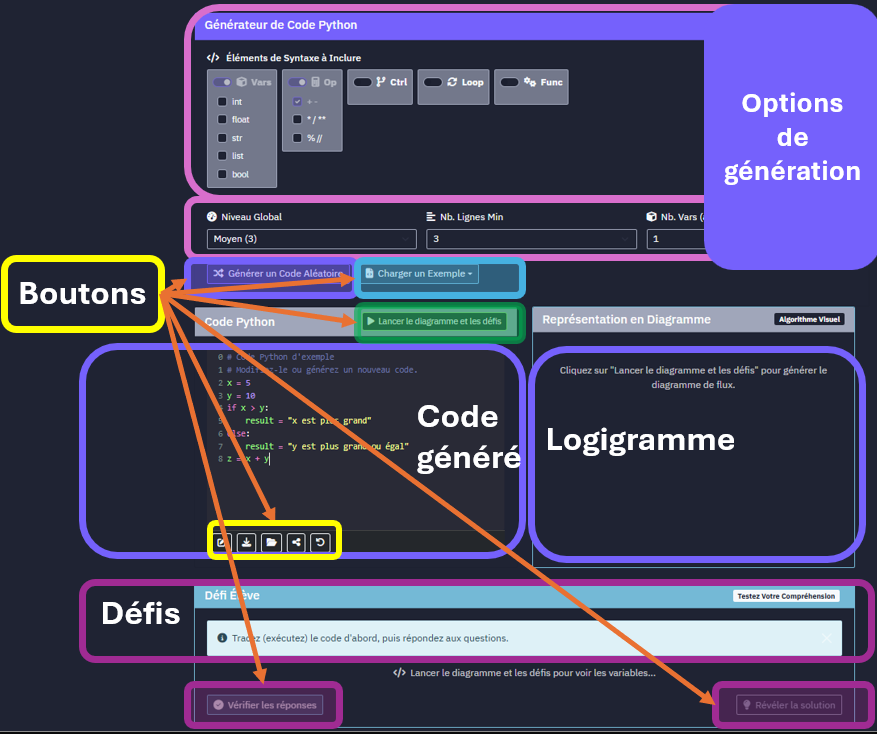
\includegraphics[width=0.99\textwidth, keepaspectratio]{app_vide_zones.png}
    \caption{Présentation générale de l'application, vierge}
    \label{app_vide_zones}
\end{figure}

On reconnaît :
\begin{itemize}
    \item Les options, à choisir dans l'interface 
    \begin{enumerate}
        \item qualitatives (les éléments syntaxiques)
        \item quantitatives (nombre de lignes, de variables et une mesure indicative de difficulté)
    \end{enumerate}
    \item Les affichages côte-à-côte du code et du logigramme
    \item En bas la section ``Défis'' correspondant à l'exercice sur le logigramme et au code
    \item Différents types de boutons
\end{itemize}
\end{minipage}


\subsubsection*{L'interface : les sorties code et diagramme}

Prenons ce code ci-dessous, généré aléatoirement avec les options 'def' \& 'def f(a)' \& 'return'.

\begin{minted}{python}
enabled = True
y = 1
def build(flag):
    output = not flag
    return output
found = build(enabled)
print("Le résultat de " + "build" + "(" + str(enabled) + ")" + " est " + str(found))
\end{minted}

Après avoir cliqué sur "Lancer le diagramme et les défis" l'utilisateur pourra visualiser le logigramme ci-dessous, qui invitera l'élève à détacher conceptuellement le flux d'exécution de la fonction de celui du programme principal, qui ici appelle effectivement la fonction qui y est définie. 
\begin{figure}[H]
    \centering
    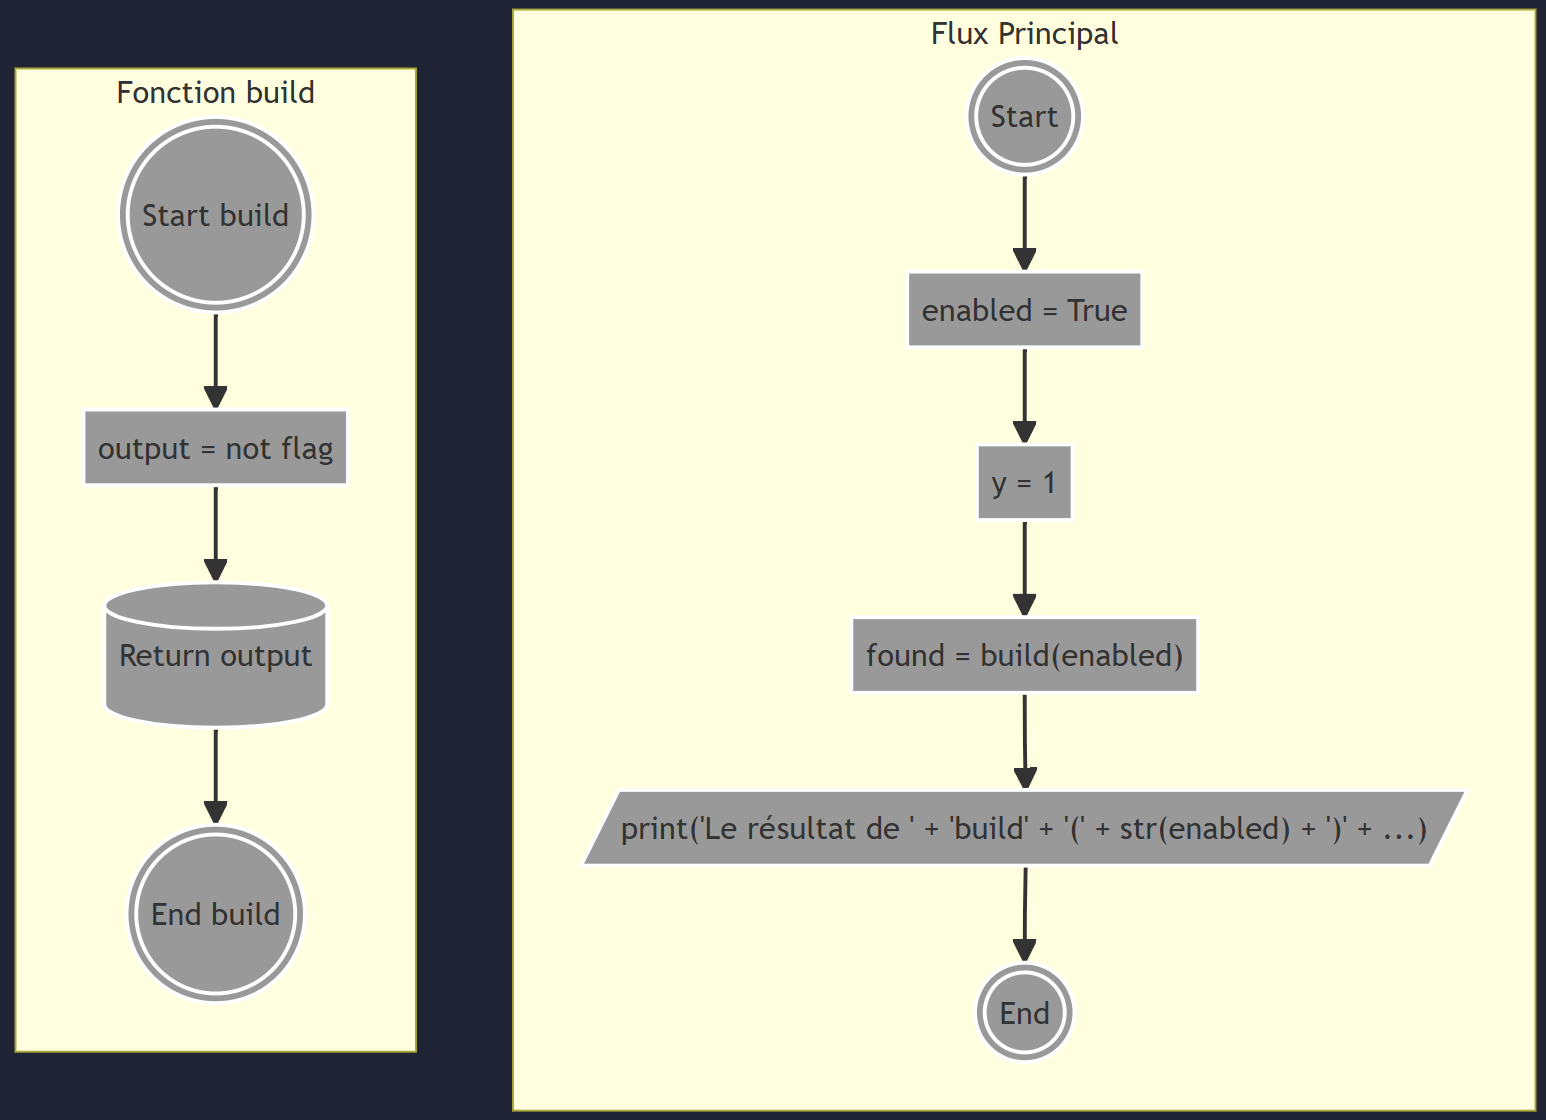
\includegraphics[width=0.8\textwidth, keepaspectratio]{Flowchart_def-f-a-return.png}
    \caption{Flowchart d'un code avec appel d'une fonction  'f(a)' \& 'return'}
    \label{Flowchart_def-f-a-return.png}
\end{figure}
On voit que la totalité de la chaîne n'est pas rendue pour des raisons d'affichage (coupée au 55ème caractère et suivie des "..." dans le parallélogramme dénotant les fonctions d'entrée/sortie).\\
Ensuite se présente la section "Défi" composée des variables à tracer.\\ Enfin l'outil propose une "Console d'exécution" qui a été ici dépliée mais qui est par défaut masquée, utile pour vérifier les sorties écran du code présenté dans l'éditeur.\\
\begin{figure}[H]
    \centering
    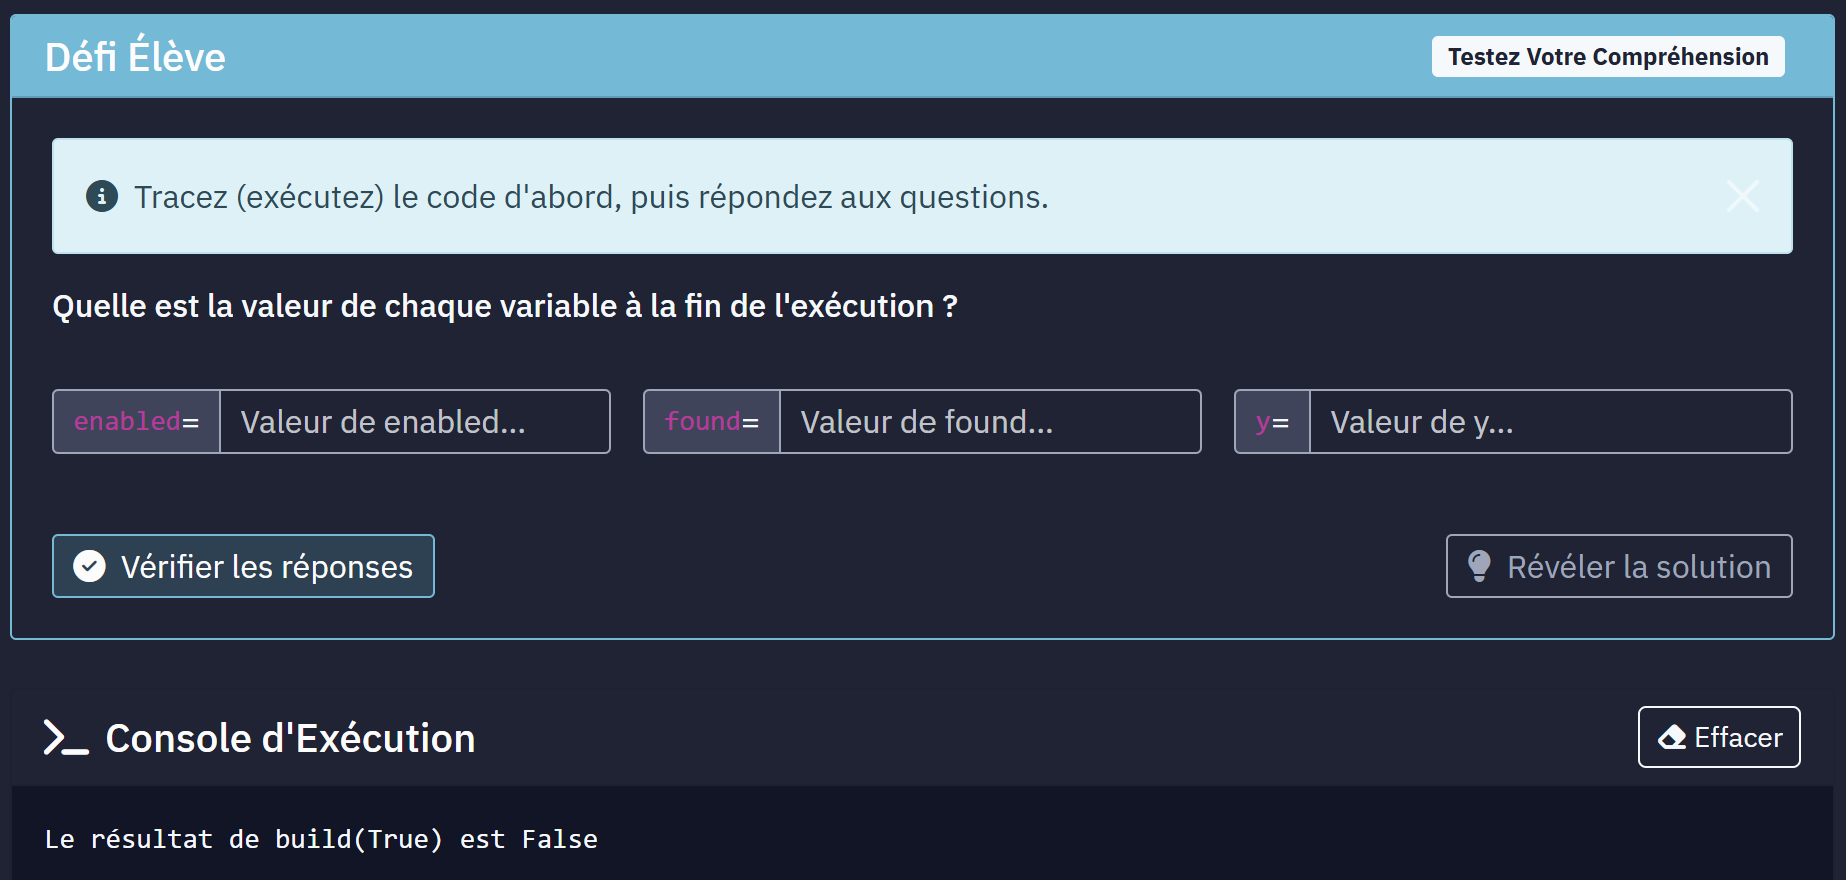
\includegraphics[width=0.8\textwidth, keepaspectratio]{Defi_Console_def-f-a-return.png}
    \caption{"Défi Élève" avec appel de fonction 'return'. La variable locale est bien absente.}
    \label{Defi_Console_def-f-a-return.png}
\end{figure}


\clearpage
\begin{minipage}{\textwidth}
\subsubsection{Les interactions entre objets : entre les \textit{cards}, entre les \textit{divs}...}
Voici un \textit{zoom} sur les options de génération de code aléatoire (explications ci-dessous) :
\begin{figure}[H]
    \centering
    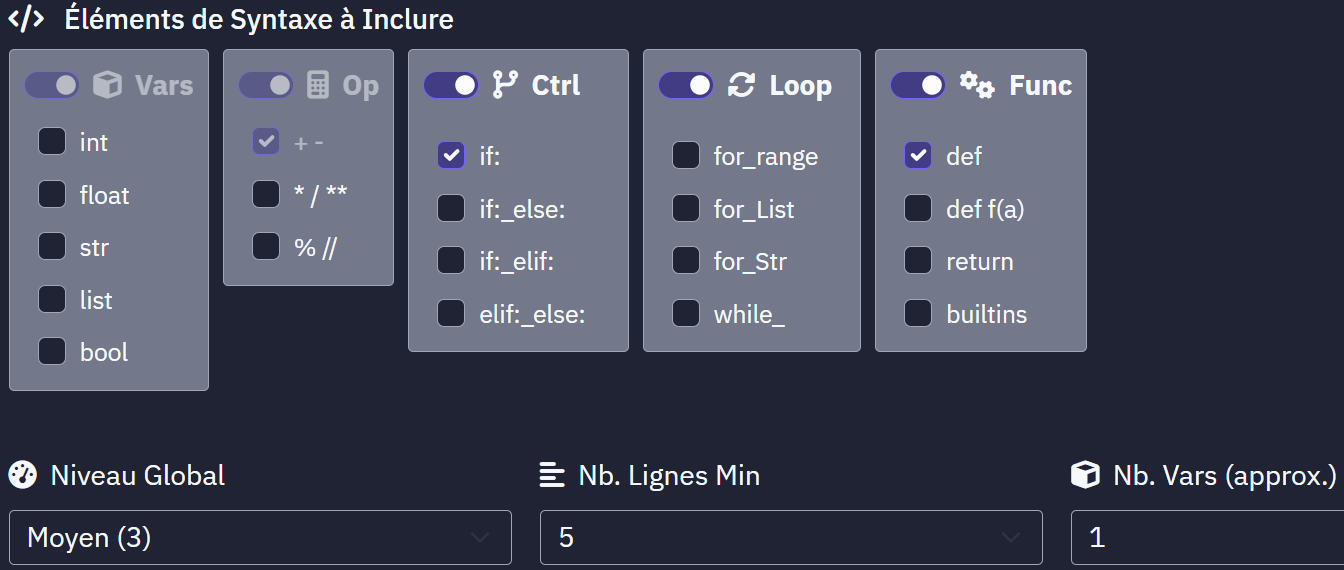
\includegraphics[width=0.8\textwidth, keepaspectratio]{ui_choix.png}
    \captionof{figure}{Présentation des choix de génération}
    \label{ui_choix}
\end{figure}

\begin{itemize}
    \item Les \textit{checkboxes} de choix des éléments syntaxiques s'affichent lorsque la \textit{card} est sélectionnée. Exemple : si 'Loop' est sélectionné l'interface déplie la \textit{card} et les différents choix de boucles sont rendus visibles.
    \item Certains choix de \textit{checkboxes} en impliquent d'autres : si 'Ctrl' est sélectionnée alors il y a forcément un 'if', si 'Func' est sélectionnée alors le code généré montrera au moins une 'def' de fonction, si 'elif:\_else' est sélectionné, le générateur de code fonctionnera forcément comme si un 'if:\_elif' avait aussi été sélectionné) $\Rightarrow$ l'interface rend visible cette logique.
    \item Certains choix de structures rendent plus naturels certains choix de types de variables: l'interface rend l'utilisateur attentif par ajout d'une classe bootstrap sur l'élément concerné (encadré vert dynamique)
    \item Les encadrés du bas présentent des critères quantitatifs qui obéissent aux choix des éléments de syntaxe (les valeurs sont recalculées dynamiquement en foncion des éléments cliqués ou non)
    \item Les encadrés du bas sont en fait des valeurs modifiables dans des listes déroulantes : les valeurs peuvent être choisies manuellement pour définir les options de génération.
\end{itemize}

\end{minipage}

\clearpage
\subsubsection{L'interface : ses éléments de choix pour la création d'un exercice}
\begin{minipage}{\textwidth}
Deux logiques indépendantes sont implémentées : 
\begin{enumerate}
    \item la génération aléatoire, opérée avec le choix des options et le bouton ``Générer un code aléatoire''
    \item l'ouverture d'un code Python pré-existant \begin{itemize}
        \item soit en chargeant un des codes pré-définis stockés actuellement dans un fichier JavaScript du projet (la figure ci-dessous montre ce bouton actionné)
        \item soit en important un fichier avec le bouton ``Ouvrir''
    \end{itemize}
\end{enumerate}

\begin{figure}[H]
    \centering
    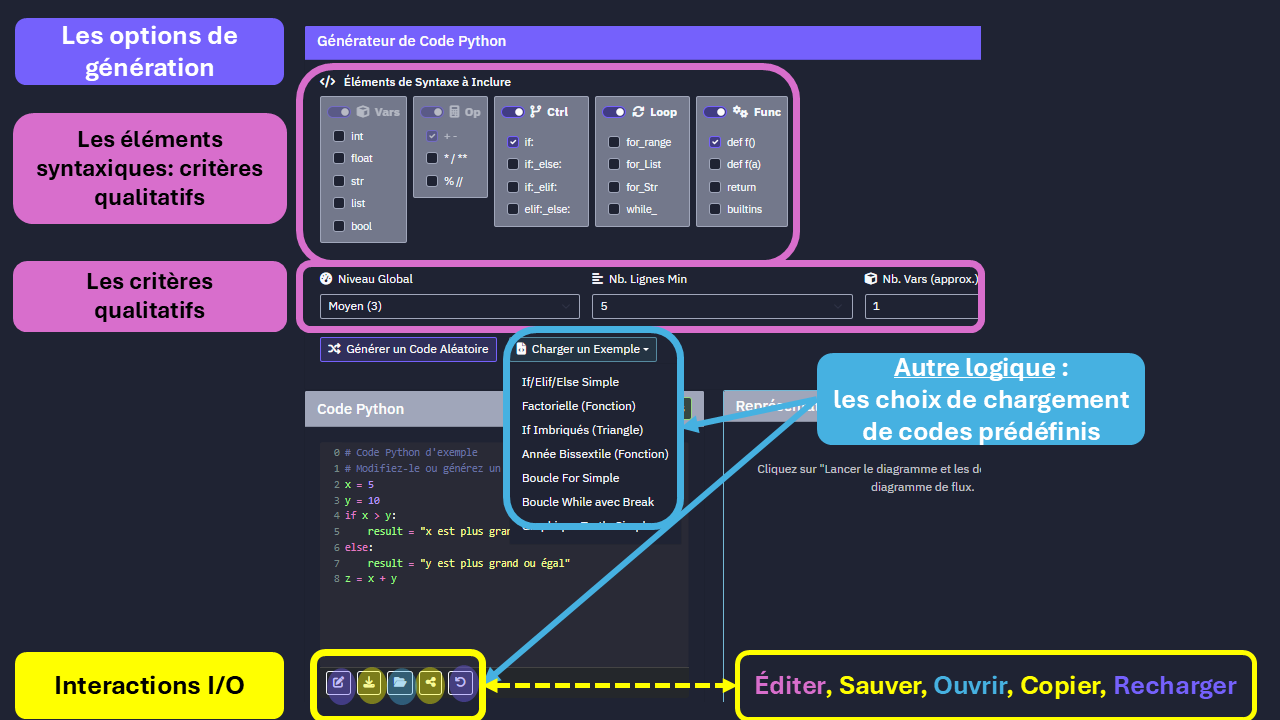
\includegraphics[width=\textwidth, keepaspectratio]{app_choix_def.png}
    \caption{Identification des éléments de choix pour la création d'un exercice}
    \label{app_choix_def}
\end{figure} 

\end{minipage}

\subsubsection{Un outil ``tout-en-un'' : fonctionnalités additionnelles}
La volonté d'aider les enseignants s'exprime dans les possibilités supplémentaires qu'offre l'outil : \begin{enumerate} 
    \item modifier le code et l'exécuter dans le navigateur : simulation d'un \code{input()} Python à l'écran (en plus de la console d'exécution déjà évoquée),
    \item sauvegarder sur disque dur le code affiché dans l'éditeur, 
    \item copier-coller dans le presse-papier le code,
    \item recharger le code tel qu'il était avant modifications (depus la dernière génération aléatoire ou depuis le dernier chargement de code pré-défini).
\end{enumerate}
\subsubsection{Les technologies employées côté client}
L'affichage des options (choix qualitatifs et quantitatifs) est géré dynamiquement par l'application de classes Bootstrap sur les éléments HTML, qui bénéficient des éléments visuels Font-Awesome.\par
L'éditeur de code est une instance CodeMirror 6 \cite{codemirror6} choisi pour ses multiples paramétrages et facilité d'intégration (par défaut à l'état \code{readOnly}). \par Le rendu graphique dans la \textit{div} Diagramme est fait grâce à  Mermaid.js qui interprète la chaîne qui est produite par l'outil à partir du code (cf. la section dévolue à cet aspect). \par L'élément clé derrière l'outil est Pyodide (portage de CPython en WebAssembly), qui rend l'exécution de Python dans le naigateur, sans installation ni problèmes logistiques potentiels de connexion à un serveur. Plus lourd que Skulpt \cite{skulpt} et Brython \cite{brython}, mais garantit une exécution Python très complète avec la plupart des modules standard, notamment ast sur lequel repose l'exécution du code et sa représentation visuelle en logigramme.

\subsection{L'architecture globale (en coulisse)}

\subsubsection{Résumé en un schéma général}
\begin{minipage}{\textwidth}
    Le processus global peut se schématiser comme ceci: 

\begin{figure}[H]
%\centering
\begin{adjustbox}{max width=\textwidth}
\begin{tikzpicture}[node distance=1.8cm, auto]
% Définition des styles
    \tikzstyle{block} = [rectangle, draw, fill=blue!20, text width=10em, text centered, rounded corners, minimum height=3em]
    \tikzstyle{action} = [rectangle, draw, fill=green!20, text width=8em, text centered, rounded corners, minimum height=2.5em]
    \tikzstyle{output} = [rectangle, draw, fill=orange!20, text width=8em, text centered, rounded corners, minimum height=2.5em]
    \tikzstyle{server} = [rectangle, draw, fill=yellow!20, text width=8em, text centered, rounded corners, minimum height=2.5em]
    \tikzstyle{line} = [draw, -latex']
    
    % Placement des nœuds de base: l'interface
    \node [block] (ui) {Interface utilisateur\\(layout.html)};
    \node [action, below of=ui, yshift=-0.5cm] (config) {Configuration des options};
    \node [block, below of=config, yshift=-0.5cm] (mainjs) {main.js};
    
    % Branches pour générer et lancer
    \node [action, below left of=mainjs, xshift=-4cm, yshift=-1cm] (generate) {Bouton "Générer un Code Aléatoire"};
    \node [action, below right of=mainjs, xshift=4cm, yshift=-1cm] (run) {Bouton "Lancer le diagramme et les défis"};
    
    % Nœuds liés à la génération de code
    \node [block, below of=generate, yshift=-0.5cm] (codegen) {code-generator.js};
    \node [output, below of=codegen, yshift=-0.5cm] (code) {code généré};
    \node [server, below of=code, yshift=-0.5cm] (logcode) {Code journalisé};
    
    % Nœuds liés au flowchart
    \node [block, below of=run, xshift=-2cm, yshift=-0.5cm] (flowgen) {flowchart-generator.js};
    \node [block, below of=flowgen, yshift=-0.5cm] (mycfg) {MyCFG.py via Pyodide};
    \node [output, below of=mycfg, yshift=-0.5cm] (flowchart) {Diagramme de flux};
    
    % Nœuds liés au défi
    \node [block, below of=run, xshift=2cm, yshift=-0.5cm] (runtrace) {runAndTraceCode\\ForChallenge()};
    \node [output, below of=runtrace, yshift=-0.5cm] (challenge) {Défi élève};
    \node [server, below of=challenge, yshift=-0.5cm] (loganswers) {Interaction élève journalisée};
    
    % Connexions
    \path [line] (ui) -- (config);
    \path [line] (config) -- (mainjs);
    \path [line] (mainjs) -- (generate);
    \path [line] (mainjs) -- (run);
    \path [line] (generate) -- node[left] {appelle} (codegen);
    \path [line] (codegen) -- node[left] {generateRandomPythonCode()} (code);
    \path [line] (run) -- (flowgen);
    \path [line] (run) -- (runtrace);
    \path [line] (flowgen) -- node[left] {triggerFlowchartUpdate()} (mycfg);
    \path [line] (mycfg) -- node[left] {to\_mermaid()} (flowchart);
    \path [line] (runtrace) -- (challenge);
    \path [line] (code) -- (logcode);
    \path [line] (challenge) -- (loganswers);
    
    % Connexions courbes ABANDONNÉES
%    \path [line] (code)      edge[bend left=30]  node[above] {affiché dans l'éditeur}   (ui);
 %   \path [line] (flowchart) edge[bend right=45] node[below] {affiché dans le panneau}  (ui);
  %  \path [line] (challenge) edge[bend right=60] node[below] {affiché dans le panneau}  (ui);
\end{tikzpicture}
\end{adjustbox}
\caption{Architecture résumée de l'exerciseur automatique}
\label{fig:architecture}
\end{figure}

\subsubsection{Résumé en quatre phrases}
Le fonctionnement du générateur repose sur une interaction entre l'interface utilisateur (HTML - CSS - JavaScript) permettant de définir les options et le moteur de génération de code (JavaScript) qui écrit sur la page dans l'éditeur de script CodeMirror. \\
\par Le fonctionnement du visualiseur logigramme se base lui sur cette chaîne de code générée, pour la traduire en un AST (Python fourni par l'environnement Pyodide) pour en extraire une sémantique traduite en une syntaxe Mermaid passée au navigateur pour être rendue sous forme graphique par Mermaid.js  \\
\par La partie "Défi" (avec l'interrogation des élèves sur la valeur des variables) est basée sur l'exécution du code (chaîne Python) dans le navigateur par Pyodide pour connaitre les variables à évaluer puis alimenter l'interface avec leur valeur et ainsi pouvoir proposer une rétroaction (HTML - CSS/bootstrap - JavaScript).\\
\par
Enfin, un \textit{back-end} de l'application a été créé par Flask pour enregistrer (\textit{journaliser}) dans une base de données relationnelle MySQL les exercices et les interactions élèves qui ont découlé de la partie "Défi".
\end{minipage}



\clearpage
\section{Présentation de la génération automatique du code}
L'objectif poursuivi est multiple : aider les élèves débutants en proposant des exercices de lecture de code, automatique et à l'infini, de niveau variable et contrôlable ; aider leurs enseignants en les déchargeant de cette charge mentale avec un outil en ligne. La plus-value pédagogique de notre outil dépend de la pertinence des codes proposés, car ceux-ci formeront le support aux exercices proposés aux élèves, c'est donc le cœur de la solution !

\subsection{Objectifs et principes directeurs du générateur}
Les critères d'une bonne génération d'exercices correspondent à différentes contraintes : \begin{itemize}
    \item \textbf{Validité et éxécutabilité :} Le code généré doit être syntaxiquement correct et s'exécuter sans erreur (sauf si une erreur logique est un objectif pédagogique explicite), afin d'être analysable par notre module \code{MyCFG.py} et compréhensible pour l'élève.
    \item \textbf{Complexité Contrôlée :} La difficulté doit être adaptable, non seulement via un niveau global, mais aussi par la sélection fine des constructions syntaxiques à inclure.
    \item \textbf{Pertinence pédagogique :} Le code doit être sémantiquement plausible et illustrer clairement les concepts visés, sans être trivial ni inutilement complexe.
    \item \textbf{Variété et aléa :} Chaque génération doit produire un code unique pour constituer une source inépuisable d'exercices  (noms, ordre des structures, opérations, appels de fonctions).
\end{itemize}

\subsection{Vue d'ensemble du processus de génération de code aléatoire et contrôlé}
La génération d'un exercice suit un flux contrôlé, orchestré par la fonction \code{generateRandomPythonCode(options)} du fichier \filepath{code-generator.js}. Ce processus peut être décomposé en quatre phases principales, comme l'illustre la figure \ref{fig:proposed_architecture_v3}.

\noindent
\begin{figure}[htbp]
\centering
\begin{tikzpicture}[node distance=1.5cm, auto]
    % Définition des styles avec la syntaxe moderne \tikzset
    \tikzset{
        block/.style = {rectangle, draw, fill=blue!20, text width=12em, text centered, rounded corners, minimum height=3em},
        phase/.style = {rectangle, draw, fill=green!20, text width=10em, text centered, rounded corners, minimum height=2em},
        line/.style  = {draw, -latex'}
    }
   
    % Phases principales - avec beaucoup plus d'espace entre elles
    \node [phase] (phase1) {1. Initialisation du générateur};
    \node [phase, below of=phase1, yshift=-.5cm] (phase2) {2. Planification \& Préparation des variables};
    \node [phase, below of=phase2, yshift=-3.5cm] (phase3) {3. Génération des structures};
    \node [phase, below of=phase3, yshift=-1.5cm] (phase4) {4. Finalisation \& remplissage};
    
    % Fonctions de l'étape 1
    \node [block, right of=phase1, xshift=4cm] (init) {Réception des inputs \& Initialisation de ses structures de données};
    
    % Fonctions de l'étape 2 - Alignées verticalement avec leur phase
    \node [block, right of=phase2, xshift=7cm] (plan1) {calculateRequiredLines};
    \node [block, below of=plan1, yshift=-.1cm] (plan2) {generateInitialVariables};
    \node [block, below of=plan2, yshift=-.1cm] (plan3) {ensureVariablesForOptions};

    
    % Fonctions de l'étape 3 - Alignées verticalement avec leur phase
    \node [block, right of=phase3, xshift=7cm] (gen1) {generateControlStructures};
    \node [block, below of=gen1, yshift=-.1cm] (gen2) {ensureTypeSpecificOperations};
    
    % Fonctions de l'étape 4 - Alignées verticalement avec leur phase
    \node [block, right of=phase4, xshift=7cm] (final1) {addFiller};
    \node [block, below of=final1, yshift=-.1cm] (final2) {finalVariableCheck};
    
    % Connexions
    \path [line] (phase1) -- (phase2);
    \path [line] (phase2) -- (phase3);
    \path [line] (phase3) -- (phase4);
    
    \path [line] (init) -- (phase1);
    
    \path [line] (phase2) -- (plan1);
    \path [line] (phase2) -- (plan2);
    \path [line] (phase2) -- (plan3);

    \path [line] (phase3) -- (gen1);
    \path [line] (phase3) -- (gen2);
    
    \path [line] (phase4) -- (final1);
    \path [line] (phase4) -- (final2);
\end{tikzpicture}
\caption{Architecture fonctionnelle du générateur de code. Le processus suit quatre phases séquentielles, chacune invoquant un ensemble de fonctions spécifiques pour planifier, générer et finaliser le code.}
    \label{fig:proposed_architecture_v3}
\end{figure}

\begin{description}
    \item[Phase 1 : Initialisation.] Le contexte de génération est préparé : les options de l'utilisateur sont lues depuis l'interface (types et nombres respectifs d'éléments : c'est l'objet \code{options}), les constantes (comme les listes de noms de variables, etc.) sont disponibles, et les structures de données pour suivre l'état du code en cours de création (lignes de code, variables déclarées) sont initialisées.
    \item[Phase 2 : Planification.] Avant d'écrire la moindre ligne de code, le générateur analyse les options pour anticiper les besoins. La fonction \code{calculateRequiredLines} estime le nombre minimal de lignes et de variables nécessaires pour satisfaire les contraintes de l'utilisateur (par exemple, une boucle \code{for} nécessite au moins deux lignes et une variable d'itération). La liste des structures est mélangée aléatoirement.
    \item[Phase 3 : Génération.] C'est le cœur du processus. Le générateur peuple le code en suivant un ordre logique : d'abord les déclarations de variables en choisissant leurs noms au hasard parmi des listes prédéfinies par type, puis les structures de contrôle. Les fonctions comme \code{ensureVariablesForOptions} et \code{generateControlStructures} sont appelées pour construire le squelette du programme.
    \item[Phase 4 : Finalisation.] Une fois les éléments principaux en place, le générateur s'assure que toutes les contraintes sont respectées. La fonction \code{ensureAllVariablesAreUsed} vérifie qu'aucune variable n'est déclarée inutilement. Ensuite, \code{addFiller} ajoute des opérations simples pour atteindre le nombre de lignes cible. Enfin, \code{finalVariableCheck} effectue une dernière passe de validation et ajoute des opérations de remplissage si besoin.
\end{description}
Ce processus structuré garantit que même si de nombreux éléments sont générés de manière aléatoire, le résultat final est toujours cohérent et conforme aux exigences pédagogiques définies par l'utilisateur.\\

Le code généré est ensuite retourné à l'interface, où l'instance CodeMirror le rend visible. Puis, indépendamment, le processus pourra continuer avec la visualisation du diagramme et la création de la section ``défis'' - qui demande de déterminer les valeurs contenues dans les variables à la fin de l'exécution du programme - et côté serveur avec la journalisation des interactions élèves.\\

NB: Le processus de génération de code constitue la branche gauche dans la figure \ref{fig:architecture} depuis le bouton ``Générer un Code Aléatoire'' jusqu'à la journalisation.

\subsection{Logique générale de la génération des structures}
Une fois passée l'étape nécessaire de création des variables (qui propose aussi des réaffectations et des premières opérations sur ces variables, cf. explications infra) les structures de contrôle sont générées selon un processus en deux phases:

\begin{enumerate}
    \item \textbf{Préparation}:
    \begin{itemize}
        \item Construction d'une liste des structures à générer (une seule de chaque sorte, par souci pédagogique) selon les options reçues de l'interface
        \item Mélange aléatoire de cette liste pour varier l'ordre d'apparition. Les structures peuvent ``piocher'' éventuellement parmi les variables disponibles (déjà déclarées dans le code généré) mais le mélange aléatoire ne provoque pas d'imbrication non voulue 
        \item Vérification et éventuellement création des variables nécessaires
    \end{itemize}
    
    \item \textbf{Génération}:
    \begin{itemize}
        \item Parcours de la liste des structures
        \item Appel de la fonction appropriée pour chaque structure : les structures se suffisent à elles-mêmes donc le fait d'en avoir plusieurs ne provoque pas d'imbrication qui ne soient pas souhaitées explicitement
        \item Gestion de l'indentation et du comptage des lignes
    \end{itemize}
\end{enumerate}

\subsection{Implémentations}
Examinons les différentes options de générations (i.e. les éléments syntaxiques disponibles) dans l'ordre où elles apparaissent dans l'interface afin d'expliquer comment est construit le code pédagogique. Dans l'interface les structures de contrôle sont regroupées en 3 sortes : les conditions dénotées '\var{Ctrl}', les boucles '\var{Loop}' regroupant \code{for} et \code{while}, enfin les fonctions '\var{Func}'.

\subsubsection{\texttt{'Vars'} \& \texttt{'Op'} : déclarations et opérations élémentaires}
L'objectif pédagogique est de découvrir les affectations de valeurs aux variables de types élémentaires, et de faire prendre conscience aux élèves que les types sont des ensembles qui viennent avec leurs opérations. Ce qui provoque l'envie de confronter les élèves à des opérations arithmétiques sur chaînes pour dévoiler la signification de la syntaxe Python : c'est ce que fait le générateur en mobilisant des opérations conformes à chaque type sélectionné.

\paragraph{Préparation des variables}
À partir des compteurs saisis (\texttt{var\_int\_count}, \texttt{var\_str\_count}, etc.), le générateur :
\begin{itemize}
  \item détermine quoi créer (\texttt{generateInitialVariables}, \href{https://github.com/edu-mateescoj/gyminf/blob/main/static/js/code-generator.js#L1083}{ligne 366}) ;
  \item garantit les quotas (\texttt{ensureVariablesForOptions}, \href{https://github.com/edu-mateescoj/gyminf/blob/main/static/js/code-generator.js#L1083}{ligne 1452}), et crée au besoin via \texttt{declareVariable} (\#168) des noms sémantiques (\texttt{generateUniqueVarName}, \href{https://github.com/edu-mateescoj/gyminf/blob/main/static/js/code-generator.js#L1083}{ligne 141}) cohérents avec le type (ex. \texttt{enabled} pour \texttt{bool}).
\end{itemize}

\paragraph{Génération des opérations}
Deux mécanismes assurent que les variables “vivent” dans le code :
\begin{itemize}
  \item \textbf{Opérations par type minimalement garanties} : \texttt{ensureTypeSpecificOperations} (\href{https://github.com/edu-mateescoj/gyminf/blob/main/static/js/code-generator.js#L1083}{ligne 1806}) force au moins une opération pertinente pour chaque type demandé (ex. \texttt{str.replace}, concaténations…).
  \item \textbf{Remplissage aléatoire jusqu’à la cible} : \texttt{addFiller} (\href{https://github.com/edu-mateescoj/gyminf/blob/main/static/js/code-generator.js#L1083}{ligne 1500}) choisit un type disponible, une variable, puis une opération parmi un éventail (\texttt{generateVariedOperation}, \href{https://github.com/edu-mateescoj/gyminf/blob/main/static/js/code-generator.js#L1083}{ligne 1586}), en évitant les répétitions.
\end{itemize}

\emph{Conséquences.} Le code contient toujours des affectations/opérations effectives, même si l’utilisateur n’active aucune structure de contrôle : cela garantit un minimum d’``activité'' à analyser. Les opérations peuvent aussi apparaître \textbf{dans} les corps des structures (cf. \texttt{generateStructureBody}, \href{https://github.com/edu-mateescoj/gyminf/blob/main/static/js/code-generator.js#L1083}{ligne 551}), ce qui renforce la variété.



\subsubsection{'\texttt{Ctrl}': les structures conditionnelles \texttt{if... elif... else:}}

\paragraph{Préparation} Si \texttt{options.main\_conditions \&\& options.cond\_if}, la structure \texttt{'if'} est ajoutée à la liste \code{structures} qui est ensuite mélangée (\href{https://github.com/edu-mateescoj/gyminf/blob/main/static/js/code-generator.js#L1083}{ligne 513}) pour assurer la variabilité d'une génération à l'autre pour simuler l'aléa.


\paragraph{Génération} Au passage, \texttt{generateIfStatement} (\href{https://github.com/edu-mateescoj/gyminf/blob/main/static/js/code-generator.js#L1083}{ligne 874}) :
\begin{itemize}
  \item génère une condition en privilégiant des variables existantes, en se limitant aux types souhaités dans le plan d'études (\texttt{generateCondition}, \#409). Ex: pour les booléens ce sont les comparaisons et opérations logiques qui sont mobilisées, pour les listes ce sont les opérateurs \code{in} ou \code{not in} et la fofnction \code{len}, etc.
  \item construit un corps non vide via \texttt{generateAppropriateStatement} (\href{https://github.com/edu-mateescoj/gyminf/blob/main/static/js/code-generator.js#L1083}{ligne 1245}), qui ajoute des opérations adaptées au contexte ;
  \item garantit qu’un \texttt{pass} est inséré si aucun type n'est disponible et que rien n’a été produit (\href{https://github.com/edu-mateescoj/gyminf/blob/main/static/js/code-generator.js#L1083}{ligne 1252}), ce qui a été utile pour le déboguage car ce cas ne devrait pas se produire.
\end{itemize}


\emph{Conséquences (aléa, imbrication, cardinalité) :} 
\begin{itemize}
  \item \textbf{Aléa} : la présence d’un \code{if}, son ordre relatif, sa condition et ses opérations internes varient d’une génération à l’autre (liste mélangée + choix stochastiques).
  \item \textbf{Imbrication} : dans la version actuelle, il n'y a pas d’\code{if} dans un \code{if}. Les corps contiennent des opérations, pas des structures récursives.
  \item \textbf{Cardinalité} : au plus \emph{une} instance de chaque sorte de structure est ajoutée par génération.
\end{itemize}


\subsubsection{'\texttt{Loop}' : les boucles \texttt{for}/\texttt{while}}
L'enjeu pédagogique du concept de boucle est majeur et il importe de proposer des codes plausibles en plus d'être valides. L'enjeu technique est la gestion appropriée des variables itérables et des itérateurs : préférence pour l'utilisation de variables déjà déclarées dans le code mais attention à la portée des variables locales, et existence ou non de conditions pré-existantes dans le code.

\paragraph{``Dispatch'' des structures} :  appel de la fonction correspondante. \\
Lors de la phase \textbf{Génération}, on parcourt la liste mélangée \code{structures} et on appelle la fonction adaptée (\href{https://github.com/edu-mateescoj/gyminf/blob/main/static/js/code-generator.js#L1083}{ligne 531} dans \code{generateControlStructures}) :
\[
\texttt{'if'} \to \texttt{generateIfStatement},\quad
\texttt{'for\_range'} \to \texttt{generateForRangeLoop},\quad
\texttt{'for\_list'} \to \texttt{generateForListLoop},\quad
\texttt{'for\_str'} \to \texttt{generateForStrLoop},\quad
\texttt{'while'} \to \texttt{generateWhileLoop},\quad
\texttt{'function'} \to \texttt{generateFunction}.
\]
Un soin particulier a été apporté aux variables d'itération. Il nous a semblé inutilement complexe que le code généré réutilise des variables existantes pour les réaffecter comme itérateur dans la création des boucles \code{for ... range}. Toutefois l'utilisation de variables déjà initialisées dans le code comme itérables nous a semblé particulièrement judicieux pour obliger les élèves à tracer chacune de ces variables et pour illustrer la réaffecation des variables et le typage dynamique Python. Ainsi :
\begin{itemize}
    \item Les noms d'itérateurs sont générés via \texttt{generateUniqueIteratorName()}
    \item Un compteur global \texttt{iteratorCounter} garantit des noms distincts
    \item Les itérateurs sont traités différemment des variables ordinaires
\end{itemize}

\subsubsection{Concrétisation d'une génération de fonction : définition et appel}

Le diagramme ci-dessous \ref{fig:genfunc_flow} illustre la séquence de décisions et d'actions prises par la fonction \methodname{generateFunction} pour construire une fonction Python complète, de la planification de sa signature à la génération de son appel.

\begin{figure}[h!]%[htbp]
\centering
% "!" signifie "adapter la hauteur proportionnellement".
\resizebox{\textwidth}{0.9\textheight}{%

\begin{tikzpicture}[
    node distance=0.5cm and 1.0cm,
    block/.style={rectangle, draw, fill=blue!20, text width=10em, text centered, rounded corners, minimum height=3.2em},
    decision/.style={diamond, draw, fill=green!20, text width=6.5em, text centered, aspect=2},
    line/.style={draw, -latex'},
    io/.style={trapezium, trapezium left angle=70, trapezium right angle=110, draw, fill=orange!20, text centered, minimum height=2.8em},
    cloud/.style={ellipse, draw, fill=gray!20, text centered, text width=6em}
]

% Phase 1: Planification
\node[block] (start) {Début \textit{generateFunction}};
\node[block, below=of start] (get_params) {1. Choisir les noms de paramètres (\#1070)};
\node[block, below=of get_params] (infer_types) {2. Inférer les types des paramètres (paramTypes)};
\node[io, below=of infer_types] (gen_def) {3. Générer def func(...)};

% Phase 2: Décisions
\node[decision, below=of gen_def] (decide_return) {4. func\_return ou difficulté ?};
\node[block, right=of decide_return, xshift=2.8cm] (set_return_true) {useReturnValue = true};
\node[block, left=of decide_return, xshift=-2.8cm] (set_return_false) {useReturnValue = false};

\node[decision, below=of decide_return] (decide_call) {5. Fonction importante ou aléa ?};
\node[decision, below=of decide_call] (check_print) {6. builtin\_print est absent ?};

% Phase 3: Corps et appel
\node[block, below=of check_print] (gen_body) {7. Générer le corps de la fonction};
\node[decision, below=of gen_body] (final_call_check) {8. shouldCallFunction ?};
\node[block, below=of final_call_check] (get_args) {9. Obtenir les arguments (ensureVariableExists)};
\node[decision, below=of get_args] (final_return_check) {10. useReturnValue ?};

\node[block, right=of final_return_check, xshift=2.8cm] (gen_assign) {11a. result = func(...)};
\node[block, left=of final_return_check, xshift=-2.8cm] (gen_simple_call) {11b. func(...)};

\node[decision, below=of gen_assign] (check_print_result) {12. builtin\_print ?};
\node[io, below=of check_print_result] (gen_print) {Ajouter print(result)};

\node[cloud, below=of gen_simple_call, yshift=-1.6cm] (end) {Fin du processus};

% Connexions
\path[line] (start) -- (get_params);
\path[line] (get_params) -- (infer_types);
\path[line] (infer_types) -- (gen_def);
\path[line] (gen_def) -- (decide_return);
\path[line] (decide_return) -- node[above] {Oui} (set_return_true);
\path[line] (decide_return) -- node[above] {Non} (set_return_false);
\path[line] (set_return_true) |- (decide_call);
\path[line] (set_return_false) |- (decide_call);

\path[line] (decide_call) -- node[left] {Oui} (check_print);
\path[line] (check_print) -- node[left] {Non} (gen_body);
\path[line] (check_print) -| node[right, pos=0.2] {Oui} (set_return_true);

\path[line] (gen_body) -- (final_call_check);
\path[line] (final_call_check) -- node[left] {Oui} (get_args);
\path[line] (get_args) -- (final_return_check);

\path[line] (final_return_check) -- node[above] {Oui} (gen_assign);
\path[line] (final_return_check) -- node[above] {Non} (gen_simple_call);

\path[line] (gen_assign) -- (check_print_result);
\path[line] (check_print_result) -- node[left] {Oui} (gen_print);
\path[line] (check_print_result) -- node[right] {Non} (end);
\path[line] (gen_print) -- (end);
\path[line] (gen_simple_call) -- (end);

% Autres chemins
\path[line] (decide_call.west) -| ++(-3.5,0) |- node[above, pos=0.9] {Non} (gen_body);
\path[line] (final_call_check.east) -| ++(3,0) |- node[above, pos=0.9] {Non} (end);

\end{tikzpicture}
}% Fin de la commande resizebox
\caption{Diagramme de flux de la logique de la fonction \textit{generateFunction}.}
\label{fig:genfunc_flow}
\end{figure}


\begin{description}
    \item[Méthodes et fonctions, avec ou sans argument] Les enseignants peuvent avoir la volonté de présenter la définition des fonctions séparément de leur appel, ou la volonté de présenter séparément les fonctions avec ou sans argument, aussi il nous est apparu important de séparer ces différents éléments dans notre interface: le choix 'func' implique que le code définisse une fonction ce qui équivaut au choix 'def f()', mais 'return' et 'def f(a)' sont les options utlisateurs qui permettront de configurer la génération de code impliquant ces éléments.\par
    Assurer que les fonctions définies ne sont pas juste des blocs de code "morts", mais qu'elles sont activement utilisées, est une propriété importante d'un bon programme. Toutefois, nous nous autorisons une certaine probabilité (paramétrable) de produire de tels codes "morts" avec des fonctions définies mais non appelées. Nous nous situons en effet au niveau de l'apprentissage de la programmation, et nous faisons l'hypothèse que susciter l'interrogation chez l'apprenant est quelque chose de productif. Nous pensons qu'il est intéressant que l'élève soit confronté à la conception naïve que le code de la fonction s'exécute dès l'écriture de sa définition, par exemple. C'est pour ça qu'il nous a semblé très important de proposer un éditeur de code dans le navigateur pour que l'élève, éventuellement guidé par l'enseignant, puisse modifier le code généré et interagir avec lui en rajoutant des print() ou des appels de fonction. Notre effort a donc porté sur comment faire pour que les fonctions définies par le générateur ne soient pas inutiles.
    
    \item[Éviter les fonctions inutiles] Si la fonction retourne une valeur (\code{useReturnValue} est true), cocher \code{builtin\_print} permet au générateur d'ajouter une ligne supplémentaire pour afficher ce résultat (le print(resultat)). Si \code{builtin\_print} n'est pas cochée, le générateur sait qu'il ne peut pas rendre l'effet d'une fonction visible via un print. Pour éviter de générer un appel de fonction "invisible" (ce qui pourrait être perçu comme pédagogiquement inutile), il va forcer \code{useReturnValue} à true. Ainsi, l'appel se fera obligatoirement avec une affectation (resultat = ma\_fonction(...)), rendant l'opération traçable pour l'élève.
    \item[Exemple] Reprenons ce code ci-dessous, généré aléatoirement avec les options 'def' \& 'def f(a)' \& 'return'.
\end{description}
\begin{minted}{python}
enabled = True
y = 1
def build(flag):
    output = not flag
    return output
found = build(enabled)
print("Le résultat de " + "build" + "(" + str(enabled) + ")" + " est " + str(found))
\end{minted}

Comment est assurée la correspondance entre les types ? et comment se fait-il que le type de la valeur de retour a un nom cohérent avec le nom de la variable ? Cette cohérence n'est pas le fruit du hasard, mais d'une chaîne logique délibérée en deux étapes qui se déroule entièrement au sein de la fonction \textit{generateFunction}. La correspondance entre le type attendu par la fonction (ici celui de \code{flag}) et le type de la variable passée en argument (ici celui de \code{enabled}) est assurée par le fait que le générateur planifie d'abord les types des paramètres lors de la définition, puis utilise ce plan pour générer à la fois la définition, le corps et pour choisir les arguments lors de l'appel. \\ Nous allons détailler le processus en traçant l'appel à \methodname{generateFunction} toujours pour notre exemple de code généré ci-dessus :
\subsubsection*{Étape 1 : Planification de la fonction et génération de sa définition)}
\begin{enumerate}
\item \textbf{Choix d'un nom de paramètre sémantique} (cf. \href{https://github.com/edu-mateescoj/gyminf/blob/main/static/js/code-generator.js#L1083}{ligne 1083}) : Évidemment la génération de la fonction commence avec un choix de nom, parmi une liste maintenue en constante pour assurer une cohérence sémantique (un verbe d’action, choisi au hasard parmi FUNCTION\_NAMES). Le processus commence donc véritablement par l’appel à \methodname{chooseAppropriateParameterNames}. Cette fonction ne choisit pas des noms au hasard, mais dans des listes thématiques (ex: dataParams = ['data', 'items', 'elements', ...], mathParams = ['x', 'y', ...]).  Pour une fonction nommée \code{build}, elle pourrait sélectionner un nom dans la liste \code{utilParams}, comme \code{flag}. Le tableau \code{params} contient maintenant \code{['flag']}.

\item \textbf{Inférence du type à partir du nom (\#1099)} : Le générateur parcourt le tableau \code{params}. Il trouve que le nom \code{flag} est inclus dans la constante \code{BOOL\_VAR\_NAMES}. Il en déduit que le type attendu est \vartype{bool}.
\begin{minted}{javascript}
// #1100
const paramTypes = params.map(param => {
// ...
    } else if (BOOL_VAR_NAMES.includes(param)) {
        return 'bool'; // <-- Le type 'bool' est inféré pour 'flag'
    } // ...
});
\end{minted}
À ce stade, le "plan" est établi : la fonction attend un paramètre de type \vartype{bool}. Le tableau \code{paramTypes} contient \code{['bool']}.

\item \textbf{Génération de la définition (\#1116)} : La ligne \code{def build(flag):} est générée en utilisant les informations du plan.

\end{enumerate}

\subsubsection*{Étape 2 : Génération de l'appel de la fonction (utilisation du plan)}
Après la logique de décision d'appeler ou non la fonction (\#1120-1138) et la génération du corps de la fonction (\#1139-1152), le générateur va dans notre exemple préparer l'appel.
\begin{enumerate}
\item \textbf{Sélection d'un argument du bon type (\#1168)} : Le code parcourt le tableau \code{paramTypes} qu'il a créé précédemment.
\begin{minted}{javascript}
// #1161
const args = params.map((param, index) => {
const paramType = paramTypes[index]; // Récupère le type planifié ('bool')
return ensureVariableExists(paramType); // Demande explicitement une variable de ce type !
});
\end{minted}
L'appel \methodname{ensureVariableExists('bool')} (\href{https://github.com/edu-mateescoj/gyminf/blob/main/static/js/code-generator.js#L189}{ligne 189}) est effectué. Cette fonction va chercher dans \code{declaredVarsByType.bool} une variable existante. Dans notre cas, elle la trouve et retourne \code{enabled}. Si elle ne l'avait pas trouvée, elle en aurait crée une
sur-le-champ en appelant \methodname{declareVariable(type)} qui suivra la même logique de création avec un nom sématiquement en ligne avec le type. Le tableau \var{args} contient maintenant \code{['enabled']}.

\item \textbf{Création de la variable de résultat (\#1171)} : La logique a déterminé que la fonction doit retourner une valeur (\code{useReturnValue} est \code{true}). Elle doit donc créer une variable pour stocker ce résultat.
\begin{itemize}
    \item \textbf{Inférence du type de retour (\#1170)} : Le type de retour est inféré à partir du type du premier paramètre. Puisque \code{paramTypes[0]} est \vartype{bool}, le type de retour est également défini comme \vartype{bool}.
    \item \textbf{Création d'une variable nommée sémantiquement (\#1171)} : Un appel à \methodname{generateUniqueVarName('bool')} est fait. Cette fonction choisit un nom sémantique dans \code{BOOL\_VAR\_NAMES}, comme \code{found}.
\end{itemize}

\item \textbf{Génération de l'appel final (\#1172)} : Le générateur assemble toutes les pièces : la variable de résultat, le nom de la fonction et l'argument, pour créer la ligne \code{found = build(enabled)}. Le code prévoit la possibilité de fonctions à plusieurs paramètres, non évoquée ici, pertinente pour une plus grande complexité.
\end{enumerate}
\par En résumé, la cohérence est le résultat d'un processus structuré : le nom sémantique du paramètre dicte son type, et ce type dicte à la fois le choix de la variable passée en argument et le nom de la variable qui reçoit le résultat (dont le type est fixé par commodité au type du premier paramètre de la fonction). Ainsi l'obtention d'un argument est obligatoirement du bon type, le tableau \var{paramTypes} agissant donc comme une "mémoire" entre la phase de définition et la phase d'appel, assurant que les deux sont synchronisées. C'est ainsi qu'un nom comme \var{is\_valid} ou \var{enabled} est choisi pour une fonction qui traitera un booléen (une information de vérité).

\subsection{Conclusion sur le processus de génération de code}

En définitive, l'architecture actuelle du générateur, qui repose sur une inférence de type à partir de noms de variables sémantiques, peut sembler inutilement complexe. Une approche alternative, plus directe, consisterait à utiliser les options de l'interface pour forcer directement la génération de types et de noms spécifiques. Par exemple : "Si options.func\_def\_a est cochée et options.var\_list\_count > 0, alors créer une fonction def process\_list(data\_list):".
Cependant, cette approche directe, bien que plus simple à concevoir initialement, présente des inconvénients majeurs rencontrés pendant le développement de notre outil, qui ont amené ce choix d'une architecture indirecte avec inférence.
\begin{description}
    \item[Explosion combinatoire et \textit{edge cases}] L'inconvénient principal de l'approche directe, qui a été rencontré très vite, est qu'elle n'a pas pu \textit{passer pas à l'échelle} de l'ajout des options et des mutiples combinaisons envisagées. Au fur et à mesure des ajouts de structures possibles, il devient de plus en plus probable que l'utilisateur choisisse des options contradictoires ou incomplètes. Atteindre la robustesse totale impose d'anticiper chaque cas, ce qui pose des questions parfois insolubles ou nécessite une résolution arbitraire. Concrètement, chaque nouvelle option ajoutée à l'interface multiplie le nombre de cas spécifiques à gérer.
    \begin{itemize}
        \item if (option A) -> faire X
        \item if (option B) -> faire Y
        \item if (option A \& option B) -> faire Z
        \item if (option A \& option C) -> faire W
        \item etc... 
    \end{itemize}
    Avec l'ambition que notre application puisse couvrir un grand nombre de syntaxes Python, le nombre de combinaisons possible a paru difficilement gérable, en tout cas la cascade de conditions imbriquées que le code était devenu paraissait impossible à maintenir et à étendre. \par Au contraire avec l'architecture actuelle par inférence le système est décomposé en règles simples et indépendantes qui collaborent.
    \begin{itemize}
        \item Règle 1 : "Choisir un nom de paramètre sémantique." (chooseAppropriateParameterNames)
        \item Règle 2 : "Déduire le type d'un paramètre à partir de son nom." (paramTypes.map(...))
        \item Règle 3 : "Pour un appel, trouver une variable existante du type requis." (ensureVariableExists)
    \end{itemize}
    Ces règles fonctionnent ensemble de manière \textit{émergente}. On n'a pas besoin de coder explicitement le cas "fonction avec un paramètre de type liste". Le système le découvre de lui-même en quelque sorte : il choisit un nom de paramètre comme \var{items} (Règle 1), en déduit que c'est une \vartype{list} (Règle 2), puis trouve une variable de type \vartype{list} pour l'appel (Règle 3). L'ajout d'une nouvelle option ne nécessite que d'ajuster une ou deux règles locales, sans casser l'ensemble du système.

    \item[Besoin d'un code "organique" et varié mais "débuggable"] L'objectif n'est pas seulement de générer du code valide (syntaxiquement correct et qui termine), mais aussi du code qui semble avoir été écrit par un humain, qui puisse simuler une certaine variété "naturelle" mais dont les structures puissent être reconnues par l'auteur (au moins au moment du développement des fonctionnalités). Une approche directe avait été essayée (ça a été la version \textit{brouillon}) mais donnait des résultats insatisfaisants : soit une variété trop faible ou à l'aspect \textit{robotique}, soit au contraire un code généré "indébuggable". En effet, en faisant appel à une génération totalement aléatoire et centralisée il devenait impossible pour l'auteur - à la simple lecture d'un code généré - de savoir d'où venaient les structures, rendant fastidieuse la phase de développement par lecture des nombreux \code{console.log} pour pouvoir tracer dans le détail l'exécution exacte. Avec l'approche finalement implémentée l'aléa est introduit à plusieurs niveaux, créant une plus grande diversité de résultats cohérents.
    \begin{itemize}
        \item Le nom de la fonction est aléatoire (calculate, process, analyze...).
        \item Le nom du paramètre est aléatoire, mais sémantiquement lié (items, data, values...).
        \item La variable utilisée pour l'appel est choisie au hasard parmi celles du bon type.
    \end{itemize}
\end{description}

Le générateur est donc ``Automatique'' au sens où le pipeline est déterministe une fois les options fixées (vérifications, utilitaires, remplissage, validation). 
\newline
Le générateur est aussi ``Aléatoire'' : noms, littéraux, ordre des structures, choix d’opérations et certaines décisions (appeler ou non la fonction) introduisent de la variabilité encadrée.
\newline
Cette cascade de choix aléatoires mais contraints produit un code qui est à chaque fois différent, tout en restant logiquement et sémantiquement correct, et qui nous semble donc convenir pour un outil pédagogique. Cette approche a été choisie car elle transforme un problème complexe de combinaisons multiples en un système de règles simples et collaboratives. Elle a été le résultat de la poursuite de nombreux objectifs contradictoires : \textit{scalabilité} et robustesse pour l'ajout de nouvelles fonctionnalités, variété mais qualité pédagogique du code généré. \\ Au final, la plus grande perte dans ce processus serait peut être - au-delà de la maintenabilité - la possibilité d'une collaboration entre collègues utilisateurs de l'outil-auteur, invités à contribuer sur le processus de développement du générateur actuel.

\clearpage
\noindent



\clearpage
\section{Présentation du traducteur automatique de code en logigramme}

Le choix du langage Python comme support d'apprentissage de la programmation tient à sa lisibilité 
et à sa large adoption en milieu scolaire.
Or le langage Python, comme d'autres langages de haut niveau, fournit un module intégré, 
\code{ast}, qui permet de décomposer du code source Python en une structure arborescente appelée 
Arbre de Syntaxe Abstraite (AST). On entend et lit souvent \textit{Arbre Syntaxique Abstrait} 
mais l'arbre n'a rien d'abstrait aussi nous dirons AST pour Abstract Syntax Tree. Cet arbre est
 une représentation hiérarchique du code qui ignore les détails syntaxiques superflus pour l'exécution
  (comme les parenthèses ou les commentaires) pour se concentrer sur la structure logique du programme. 
  Chaque nœud de l'AST correspond à une construction du langage : une assignation, une condition, une boucle,
   un appel de fonction, etc. \\

Dans le contexte de l'apprentissage de la programmation, la visualisation des structures de contrôle est un 
outil pédagogique fondamental. Nous faisons l'hypothèse que le passage d'un langage à un autre est un travail 
stimulant les compétences qui forment la si élusive \textit{pensée computationnelle}. Le logigramme, ou 
diagramme de flux, ou \textit{flowchart} offre une représentation graphique - certes plus intuitive - de 
l'algorithmique sous-jacente à un programme, mais il est constitué d'éléments syntaxiques à apprendre. 
Chaque élément syntaxique Python n'a pas sa correspondance un-pour-un dans la syntaxe logigramme, et la finalité du logigramme est de rendre compte de l'exécution du flux de contrôle \textbf{logique} du programme. \\
Notre implémentation \code{MyCFG.py} est conçue pour analyser du code source Python fournie sous forme de chaîne, construire un graphe de flux de contrôle (\textit{CFG, pour Control Flow Graph}, et le traduire en une syntaxe de diagramme Mermaid. L'objectif principal est de fournir un retour visuel immédiat aux apprenants dans un environnement d'exercice interactif, en mettant l'accent sur la clarté pédagogique plutôt que sur une analyse exhaustive de tous les aspects du langage.

\subsection{L'AST Python}
Pour traduire un programme textuel en un CFG, il est nécessaire d'en extraire la structure logique. Plutôt que de recourir à une analyse fragile basée sur des expressions régulières, nous avons adopté une approche robuste et standard en informatique : l'analyse de l'AST.

\subsection{AST, CFG, et logigramme}
La génération d'un logigramme à partir d'un code source est un processus de traduction qui transforme une 
représentation purement syntaxique en une représentation sémantique du flux d'exécution. Notre module 
\code{MyCFG.py} opère cette traduction. Détaillons les fondements théoriques de cette transformation et illustrons 
comment notre implémentation l'a concrétisée.
\hline
Prenons un code minimal:
\begin{minted}{python}
x = 1
if x > 0:
    y = 1
else:
    y = -1
print(y)
\end{minted}
Lorsqu'un interpréteur Python lit un script, sa première étape est de le \textit{parser} (analyser syntaxiquement). 
Ce processus convertit la chaîne de caractères brute en cette structure de données hiérarchique qu'est l'AST.
Le \code{dump} de l'AST pour ce code minimal est :
\begin{verbatim}
    Module(body=[Assign(targets=[Name(id='x', ctx=Store())], value=Constant(value=1)), If(test=Compare(left=Name(id='x', ctx=Load()), ops=[Gt()], comparators=[Constant(value=0)]), body=[Assign(targets=[Name(id='y', ctx=Store())], value=Constant(value=1))], orelse=[Assign(targets=[Name(id='y', ctx=Store())], value=UnaryOp(op=USub(), operand=Constant(value=1)))]), Expr(value=Call(func=Name(id='print', ctx=Load()), args=[Name(id='y', ctx=Load())], keywords=[]))], type_ignores=[])
\end{verbatim}
que nous préférons immédiatement représenter d'une façon plus humaine, plus lisible car déjà arborescente. 
On voit bien que le Module de l'AST est la racine. Elle contient une liste d'instructions (body) qui sont soit des
 affectations (Assign), soit une condition (If) ou un appel de fonction (Expr avec Call).
\begin{verbatim}
    Module(
  body=[
    Assign(
      targets=[
        Name(id='x', ctx=Store())],
      value=Constant(value=1)),
    If(
      test=Compare(
        left=Name(id='x', ctx=Load()),
        ops=[
          Gt()],
        comparators=[
          Constant(value=0)]),
      body=[
        Assign(
          targets=[
            Name(id='y', ctx=Store())],
          value=Constant(value=1))],
      orelse=[
        Assign(
          targets=[
            Name(id='y', ctx=Store())],
          value=UnaryOp(
            op=USub(),
            operand=Constant(value=1)))]),
    Expr(
      value=Call(
        func=Name(id='print', ctx=Load()),
        args=[
          Name(id='y', ctx=Load())],
        keywords=[]))],
  type_ignores=[])
\end{verbatim}
Cette arborescence pourra être résumée sous une forme presque lisible ci-dessous :
\begin{verbatim}
Module
├─ Assign: Name('x', Store) := Constant(1)
├─ If (test: Compare(Name('x', Load) > Constant(0)))
│  ├─ Assign: Name('y', Store) := Constant(1)
│  ├─ else:
│  └─ Assign: Name('y', Store) := UnaryOp(-, Constant(1))
└─ Expr: Call(Name('print', Load), [Name('y', Load)])
\end{verbatim}
Cette dernière écriture de l'AST est lisible car elle fait apparaitre des noeuds qui structurent notre lecture mais
chacun de ces noeuds correspondent à une construction syntaxique du langage. Chaque nœud a des attributs qui décrivent ses 
composants (ex. \code{targets}, \code{value} pour une affectation).
Cet arbre est une description parfaite de \textit{ce qu'est} le code, mais pas de \textit{comment il s'exécute}. 
Par exemple, il ne montre pas explicitement que la branche \code{orelse} est une alternative à la branche 
\code{body}, ni que l'exécution continue après la structure \code{If}. \par  L'AST est une représentation statique et 
hiérarchique. Le CFG, quant à lui, est une représentation graphique du flux d'exécution.
On a vu que l'AST était un arbre : c'est un graphe non dirigés, acyclique et connexe (les éléments sont tous reliés).
Comme l'illustre l'implémentation \code{PyCFG.py} de \textit{The Fuzzing Book}, un CFG est un graphe dirigé, non
connexe et potentiellement cyclique (dès qu'une itération est présente) où :
\begin{itemize}
    \item Les \textbf{nœuds} représentent des blocs d'instructions exécutés séquentiellement sans branchement.
    \item Les \textbf{arêtes} représentent les transferts de contrôle (sauts) entre ces blocs.
\end{itemize}
Tant que le CFG fourni par le module ast de Python n'a pas été ``visité'' il est vide:
\begin{verbatim}
--- CFG : les noeuds ---
[]
--- CFG : les arêtes ---
set()
\end{verbatim}
Une fois la ``visite'' effectuée on a construit un CFG :
\begin{verbatim}
    --- CFG : les noeuds ---
[('node01', 'Start'), ('node02', 'x = 1'), ('node03', 'x > 0'), ('node04', 'y = 1'), ('node05', 'y = -1'), ('node06', '.'), ('node07', 'print(y)'), ('node08', 'End')]
--- CFG : les arêtes ---
{('node02', 'node03', ''), ('node04', 'node06', ''), ('node03', 'node05', 'Non'), ('node06', 'node07', ''), ('node03', 'node04', 'Oui'), ('node01', 'node02', ''), ('node07', 'node08', ''), ('node05', 'node06', '')}
\end{verbatim}
On dira que le CFG est l'ensemble de ces noeuds et de ces arêtes : il rend explicite la notion de \textbf{flux},
 il n'est plus hiérarchique mais séquentiel, avec des branches et des fusions, qu'il nous appartient de visualiseur
 pour l'élève.

\subsection{Pourquoi PyCFG (Fuzzing Book) était utile mais insuffisant pour nos objectifs}
\paragraph{Apports de PyCFG :}
\begin{itemize}
\item Démonstration claire de la \textbf{construction d’un CFG à partir de l’AST} (\textit{The Fuzzing Book} \cite{fuzzingbook}).
\item Base technique pour le parcours \textit{visitor}, gestion des blocs, arêtes et séquences.
\end{itemize}

\paragraph{Limites pour l’usage pédagogique visé (et adaptation \code{MyCFG.py}).}
\begin{itemize}
\item \textbf{Granularité trop bas niveau}: PyCFG reflète étroitement la syntaxe (blocs techniques), alors que 
nous visons des \textbf{concepts algorithmiques} lisibles (\code{Process}/\code{Decision}/\code{Junction}/\code{IoOperation}).
\item \textbf{Absence de nœuds de jonction} explicites pour la convergence visuelle des branches ; 
\code{MyCFG} insère des \code{Junction} dédiés, pour réduire la charge cognitive en fournissant à l'élève des repères 
visuels clairs et pour visuellement éviter les croisements illisibles au moment du rendu par l'algorithme Mermaid.
\item \textbf{Sortie Graphviz} : adaptée à la recherche mais moins \textit{portable web} ; nous ciblons \textbf{Mermaid}
 pour un rendu immédiat dans le navigateur, sans dépendances serveur pour cette partie du projet.
\item \textbf{Sémantique pédagogique ajoutée par MyCFG} : typage léger des I/O en conformité avaec ce qui est fait
en classe, des libellés plus ``human-friendly'', une séparation en \code{subgraph} pour séparer le flux principal
des définitions de fonctions, ce que PyCFG ne vise pas.
\item \textbf{Contrôle de la ``verbosité'' par MyCFG} : heuristiques pour condenser les expressions (ex. 
conditions courtes, noms de variables) afin d'essayer de garder le diagramme lisible.
\end{itemize}

\paragraph{Conclusion :} PyCFG fournit l’ossature algorithmique ; \code{MyCFG.py} ajoute une \textbf{couche sémantique
 et ergonomique} nécessaire à un \textit{retour visuel immédiat et didactique} pour les élèves, directement dans 
 le navigateur via Pyodide + Mermaid, conformément à l'objectif de traduction du code dans le navigateur.

 
\subsubsection{Le choix de l'AST comme source de vérité}
Le module \code{ast} de la bibliothèque standard Python permet déjà de transformer une chaîne de code source en une 
structure arborescente (l'AST) qui représente sans ambiguïté les relations entre les différentes instructions. 
Ce choix présente plusieurs avantages déterminants :
\begin{itemize}
    \item \textbf{Robustesse :} L'analyseur de Python fait le travail complexe de validation de la syntaxe. Notre traducteur opère sur une structure déjà validée.
    \item \textbf{Précision sémantique :} L'AST ne représente pas le texte, mais sa signification. Un nœud \code{ast.For} est distinct d'un nœud \code{ast.While}, et nous pouvons exploiter cette distinction pour analyser l'arbre, même si leur rendu textuel est arbitraire et peut varier d'une implémentation à l'autre.  
    \item \textbf{Extensibilité :} L'approche est modulaire. Pour supporter une nouvelle construction du langage (par exemple, \code{try...except}), il suffit d'ajouter une méthode pour traiter le nœud AST correspondant (\code{ast.Try}), sans impacter le reste du code, implémentée dans l'approche "visiteur".
\end{itemize}

\subsubsection{Le \textit{template} (patron de conception) "Visiteur"}
Pour parcourir l'AST, nous utilisons le patron de conception \textit{Visiteur}. La classe \code{ControlFlowGraph} implémente une méthode \code{visit(node, parent\_id)} qui agit comme un répartiteur. Selon le type du nœud AST visité (ex: \code{ast.If}), elle délègue le traitement à une méthode spécialisée (ex: \code{visit\_If}). Cette approche structure le code de manière claire et alignée sur la grammaire du langage Python.

Notre approche s'inspire de projets académiques et open-source qui exploitent l'AST pour l'analyse de code, 
notamment les travaux présentés dans \textit{The Fuzzing Book} par Zeller et al. \cite{fuzzingbook}, qui 
démontrent la construction d'un CFG à partir d'un AST. De même, la documentation \textit{Green Tree Snakes} 
\cite{greentreesnakes} illustre la puissance de la manipulation et de la visite de l'AST pour des tâches 
d'analyse statique. Notre \code{MyCFG.py} adopte une philosophie similaire en utilisant le patron de conception 
\textit{Visiteur} pour parcourir l'AST. Une méthode de visite spécifique est implémentée pour chaque type de 
nœud AST pertinent, permettant de traduire progressivement la structure du code en une structure de graphe 
composée de nœuds et d'arêtes.


 \clearpage
\subsection{Vocabulaire AST et sémantique des nœuds du CFG}

La traduction d'un AST en un CFG implique une cartographie entre les nœuds syntaxiques de l'AST et les nœuds sémantiques du logigramme. Nous avons défini un ensemble de types de nœuds internes à notre graphe, chacun correspondant à un ou plusieurs types de nœuds AST et représentant un concept algorithmique distinct. Le tableau \ref{tab:node-types} détaille cette correspondance pour les éléments actuellement implémentés dans \code{MyCFG.py}.

\begin{longtable}{| p{3cm} | p{4cm} | p{8cm} |}
\caption{Correspondance des Types de Nœuds Internes, Nœuds AST et Sémantique}\label{tab:node-types}\\
\hline
\textbf{Node Type (Interne)} & \textbf{Nœud(s) AST Correspondant(s)} & \textbf{Sémantique (Langage Naturel)} \\
\hline
\endfirsthead
\hline
\endfoot
\hline
\multicolumn{3}{r}{\small\slshape Table suite en page suivante} \\
\hline
\endlastfoot
% --- Types Implémentés --- & & \\ \hline
StartEnd & \code{ast.Module} (implicite), \code{ast.FunctionDef} (implicite) & Représente le point d'entrée ('Start') ou de sortie ('End') global du script/module ou d'une fonction spécifique. \\ \hline
Decision & \code{ast.If}, \code{ast.While}, \code{ast.For} & Nœud où le flux de contrôle se divise en fonction d'une condition (If, While) ou de l'état d'une itération (For). Représenté par un losange. \\ \hline
Process & \code{ast.Assign}, \code{ast.Expr} (contenant \code{ast.Call}), \code{ast.Pass} (via \code{generic\_visit}) & Représente une étape d'exécution séquentielle : une affectation, l'évaluation d'une expression, un appel de fonction, ou une instruction vide. Représenté par un rectangle. \\ \hline
Junction & N/A (Nœud structurel ajouté par notre visiteur pour améliorer le rendu graphique et la lisibilité) & Point de convergence où plusieurs chemins d'exécution se rejoignent (typiquement après une structure \code{if}/\code{else}). Assure la clarté du flux en unifiant les branches. Représenté par un petit cercle. \\ \hline
Return & \code{ast.Return} & Indique la fin de l'exécution d'une fonction et le retour d'une valeur. Termine le chemin d'exécution dans cette fonction. \\ \hline
Jump & \code{ast.Break}, \code{ast.Continue} & Représente un saut inconditionnel dans le flux de contrôle vers un autre point défini (sortie de boucle pour 'Break', début de l'itération suivante pour 'Continue'). Termine le chemin séquentiel local. \\ \hline
IoOperation & \code{ast.Call} (avec \code{func.id} étant 'print' ou 'input') & Un sous-type de 'Process' pour distinguer sémantiquement les opérations d'entrée/sortie, souvent représentées par un parallélogramme. \\ \hline
\end{longtable}

\subsection{Philosophie et architecture de \textit{MyCFG.py}}

L'architecture de \code{MyCFG.py} est guidée par une philosophie centrée sur l'objectif pédagogique. Plutôt que de viser une représentation exhaustive de tous les mécanismes d'exécution de Python (comme la gestion des exceptions, les définitions en compréhension ou l'asynchronisme), notre implémentation se concentre sur les constructions algorithmiques fondamentales enseignées aux débutants.

\paragraph{Séparation des préoccupations.} La classe \code{ControlFlowGraph} est conçue en trois phases distinctes :
\begin{enumerate}
    \item \textbf{Initialisation et Parsing :} Le constructeur (\code{\_\_init\_\_}) prend le code source en entrée et utilise \code{ast.parse()} pour générer l'AST. La gestion des erreurs de syntaxe est effectuée à ce stade précoce, avec un retour immédiat si le code est syntaxiquement invalide. Ne sont pas capturées ici les erreurs sémantiques (exemple: l'utilisation dans une syntaxe Python valide de variables non initialisées)
    \item \textbf{Construction du Graphe (Visite de l'AST) :} La méthode \code{visit} et ses sous-méthodes spécialisées (\code{visit\_If}, \code{visit\_For}, etc.) parcourent l'AST. Cette phase ne fait qu'ajouter des nœuds et des arêtes aux structures de données internes (\code{self.nodes}, \code{self.edges}). C'est ici que la logique de traduction de la syntaxe en flux de contrôle est implémentée. Une caractéristique clé est l'ajout de nœuds de \textbf{jonction} structurels, qui ne correspondent à aucun nœud AST mais sont essentiels pour représenter la convergence des flux de manière claire, notamment après les blocs conditionnels.
    \item \textbf{Sérialisation en Mermaid :} La méthode \code{to\_mermaid} lit les structures de données internes (nœuds et arêtes) et génère la chaîne de caractères finale au format Mermaid. Cette séparation garantit que la logique de construction du graphe est indépendante du format de sortie final.
\end{enumerate}

\paragraph{Gestion des portées et des sous-graphes.} Une décision architecturale importante a été de séparer visuellement le flux principal du script des définitions de fonctions. \code{MyCFG.py} utilise une pile de portées (\code{\_function\_scope\_stack}) pendant la visite de l'AST pour identifier quels nœuds appartiennent à quelle fonction. Lors de la sérialisation en Mermaid, cette information est utilisée pour générer des \code{subgraph} distincts, améliorant considérablement la lisibilité en évitant le croisement d'arêtes entre des contextes d'exécution logiquement séparés.

\paragraph{Représentation pédagogique des boucles.} Pour les boucles \code{for}, une attention particulière a été portée à la représentation. Plutôt qu'un simple nœud de décision, nous avons choisi de décomposer la boucle en une structure plus détaillée inspirée des logigrammes classiques (voir figure \ref{foreach_flowchart} : un test initial de vacuité de l'itérable ("des éléments sont ils présents dans la structure sur laquelle itérer"?), l'initialisation de la variable d'itération (l'itérateur), l'exécution du corps, un test de continuation, et la mise à jour de la variable. 
\begin{figure}[H]
    \centering
    \begin{subfigure}{0.45\textwidth}
         \centering
         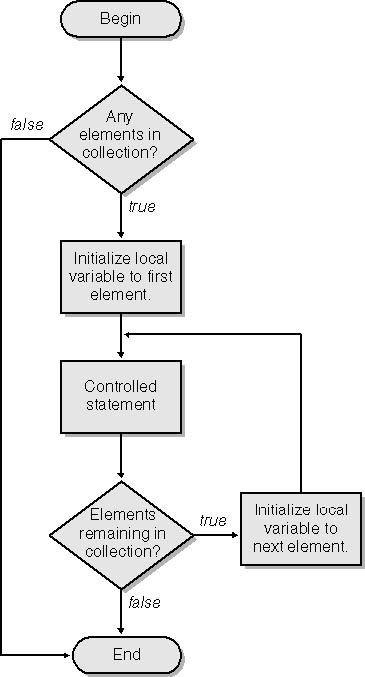
\includegraphics[width=0.3\textwidth]{FqKSJ.jpg}
        \caption{Exemple de flowchart "for each" \cite{for_each_exemple}}
        \label{fig:foreach_flowchart}
    \end{subfigure}
    \begin{subfigure}{0.45\textwidth}
        \centering
        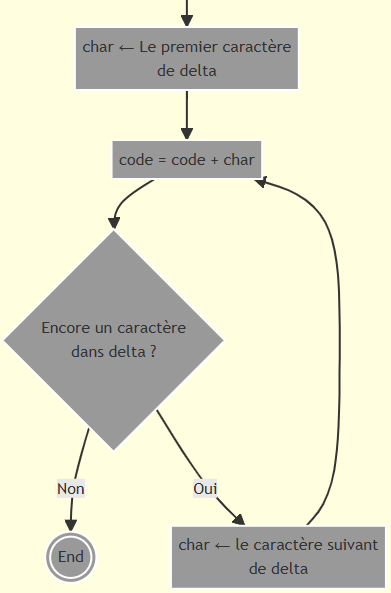
\includegraphics[width=0.3\textwidth]{for_str_screenshot.png}
        \caption{Copie d'écran d'une partie de logigramme visualisant une boucle ``for ... str''}
        \label{fig:for_str_screenshot}
    \end{subfigure}
    \caption{Comparaison de notre ``for ... in <str>'' avec un exemple de ``for each''}
    \label{fig:deux_for}
\end{figure}

Cette décomposition, bien que plus verbeuse, vise à rendre le mécanisme d'itération plus explicite pour l'apprenant. Une heuristique est également utilisée pour décrire la nature de l'itérable (chaîne, liste, variable, etc.) et de ses éléments (caractère, nombre, etc.) en langage naturel. C'est peut être encore un peu trop verbeux malgré l'attention qui a été porté pour réduire la longueur des chaînes (exemples: utiliser les ' plutôt que les ", couper les longues chaines et les faire suivre de ``...'')

\paragraph{Robustesse et limitations.} L'implémentation actuelle gère les structures de contrôle de base (\code{if}/\code{else}, \code{for}, \code{while}), les assignations, les appels de fonction, et les sauts (\code{break}, \code{continue}, \code{return}). Elle ne gère pas encore les constructions plus avancées comme la gestion des exceptions (\code{try}/\code{except}/\code{finally}), les contextes (\code{with}), les classes, ou les fonctionnalités asynchrones. Cette limitation est suffisante pour couvrir un sous-ensemble du langage pertinent pour les exercices du niveau des élèves, de débutant à intermédiaire.

\subsection{Fonctionnement de l'application pour la traduction de codes en logigramme}

Essayons de situer plus globalement l'instance CFG (Python) dans le contexte de la traduction d'un code source issu du navigateur (JS) et rendu graphiquement par Mermaid.js à l'aide du graphique ci-dessous.

Citation de la doc officielle Pyodide \cite{pyodide}:
\begin{quote}
    When we proxy a JavaScript object into Python, the result is a JsProxy object.\\ When we proxy a Python object into JavaScript, the result is a PyProxy object.
\end{quote}

\begin{landscape}
\begin{figure}
    \centering
    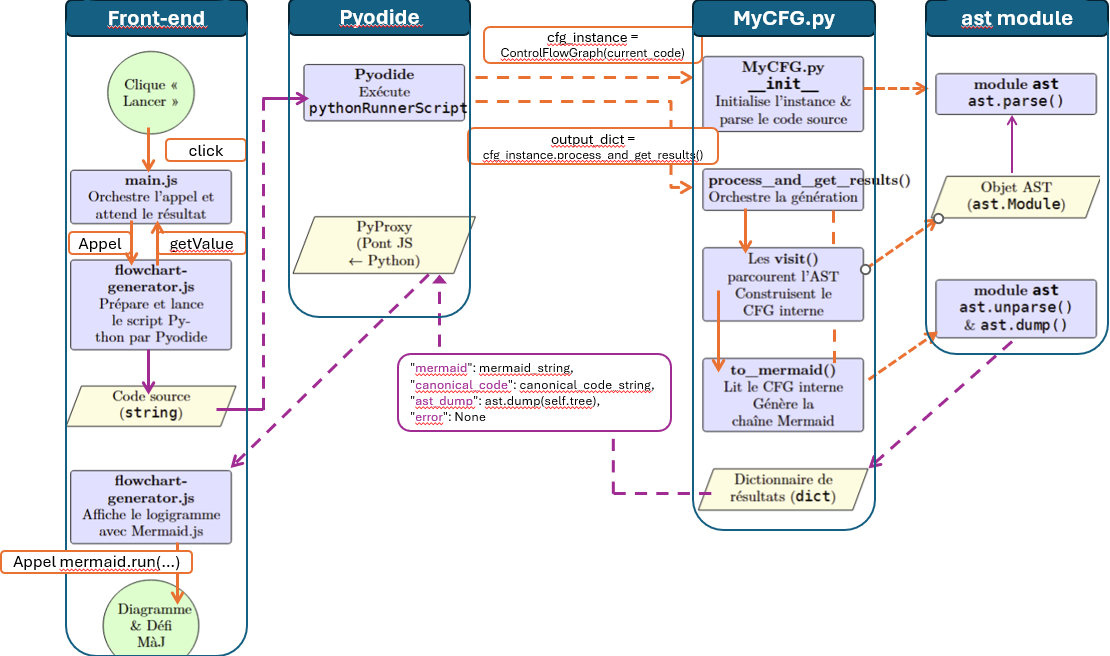
\includegraphics[width=1.3\textwidth]{BPMN_process_logigramme.png}
    \caption{Génération du logigramme: Business Process Model des appels et des objets retournés}
    \label{bpmn}
\end{figure}
\end{landscape}

\newpage

\clearpage
\section{Présentation des interactions élèves et de leur journalisation }

L'enjeu de la didactique est de pouvoir fournir aux apprenants la réponse appropriée pour favoriser leur apprentissage. Notre interface \textit{full front-end}, qui confronte les élèves à des exercices de traçage de code de difficulté variable et mobilisant des éléments de syntaxe Python de façon contrôlée, en leur proposant une évaluation formative par rétroaction immédiate, se positionne comme un outil-auteur capable de délivrer déjà un environnement d'apprentissage assez riche.  \par 
La possibilité de plus-value apportée par l'enregistrement des codes générés, des modifications faites dans l'éditeur, des éventuelles réponses proposées par l'élève ou la révélation des solutions et leur \textit{timing} s'inscrit dans l'ambition didactique formulée par Qian et Lehman (2017) \cite{Qian_Lehman_2017} :
\begin{quote}we recommend that computing education research move beyond documenting misconceptions to address the development of students' (mis)conceptions [...] \end{quote}

Alors que l'enseignement de la programmation est maintenant proposée à des cohortes massives d'élèves (tous les élèves du secondaire de filière académique, à notre connaissance dans tous les pays de l'OCDE) nous rejoignons leur postulat : 
\begin{quote}we believe that developing and enhancing instructors’ [...] ability to apply effective instructional approaches and tools to address students’ difficulties, is vital to the success of teaching introductory programming.\end{quote}

\subsection{Principes directeurs de la collecte de données}
Il serait évidemment intéressant de pouvoir évaluer l'efficacité de dispositifs didactiques permis par notre outil, en classe et en dehors, et de pouvoir analyser l'évolution des élèves. Cela nécessite un système de journalisation (\textit{logging}) robuste et réfléchi.

\subsubsection{Une base de données à double vocation pédagogique et didactique}
La collecte de données dans un contexte éducatif répond à une double finalité. D'une part, elle a une \textbf{vocation pédagogique} : en assurant une gestion fiable et éthique des utilisateurs, elle permet de tracer le parcours individuel de chaque élève pour lui fournir une rétroaction personnalisée et suivre sa progression. D'autre part, elle a une \textbf{vocation didactique} : en agrégeant des données riches et fiables sur les interactions, elle ouvre la voie à des analyses à plus grande échelle sur les stratégies d'apprentissage, les erreurs fréquentes et l'efficacité des exercices proposés.\\ 
L'architecture de notre base de données et de notre système de journalisation a été conçue pour servir ces deux objectifs, sous deux contraintes majeures.

\subsubsection{Contraintes techniques et éthiques}
Des \textbf{contraintes d'anonymat} strictes doivent être appliquées relatives à l'absence de traçage : le mot de passe rentré par l'utilisateur n'est jamais stocké en clair mais haché avec Bcrypt, le compte utilisateur n'est pas croisé avec d'autres identifiants et plus généralement les données utilisateurs collectées n'existent que pour le traitement pédagogique des interactions entre l'élève et le défi qui lui est proposé. Il appartiendra à l'enseignant de dé-anonymiser les informations reçues dans le cadre de sa relation avec ses apprenants, dans le respect de son \textit{contrat didactique}. Par ailleurs, pour augmenter les chances de récolter des données riches, en grand nombre, nous voulons proposer \textbf{une expérience utilisateur de qualité} à l'image de ce à quoi sont habitués les élèves dans leur vie quotidienne, pour augmenter l'engagement des apprenants. Ceci nous contraint à utiliser les bonnes pratiques de développement web moderne pour la gestion des utilisateurs et pour les interactions de journalisation qui doivent être asynchrones, sans blocage ni rechargement de la page entière lorsque l'utilisateur est dans l'interface.

\subsubsection{Une preuve de concept extensible}
Le système de journalisation actuel doit être considéré comme une \textbf{preuve de concept} fonctionnelle. Il met en place l'infrastructure technique complète pour capturer une variété d'événements (génération de code, exécution, vérification de réponses, etc.) et répond déjà à des besoins identifiés, certes de façon assez intuitive par l'auteur et ses collègues après des échanges informels. Nous insistons ici sur le fait que le travail d'analyse didactique pour définir des \textbf{indicateurs de performance pertinents} et des métriques d'apprentissage complexes reste à l'heure actuelle un champ de recherche ouvert. L'architecture mise en place est intentionnellement modulaire pour permettre l'ajout futur de nouveaux types d'événements et d'analyses plus fines, à mesure que la recherche sur les indicateurs progressera.

\subsubsection{Présentation visuelle de la collecte de données et des relations}
Revoici l'UI, avec mise en évidence des éléments qui provoquent la collecte des données, déclenchée par chacun des ``clics'', ici mis en valeur par un petit rectangle plein (les couleurs font référence aux logiques appelées: génération; chargement; création du défi; interaction avec l'exercice).

\begin{figure}[H]
    \centering
    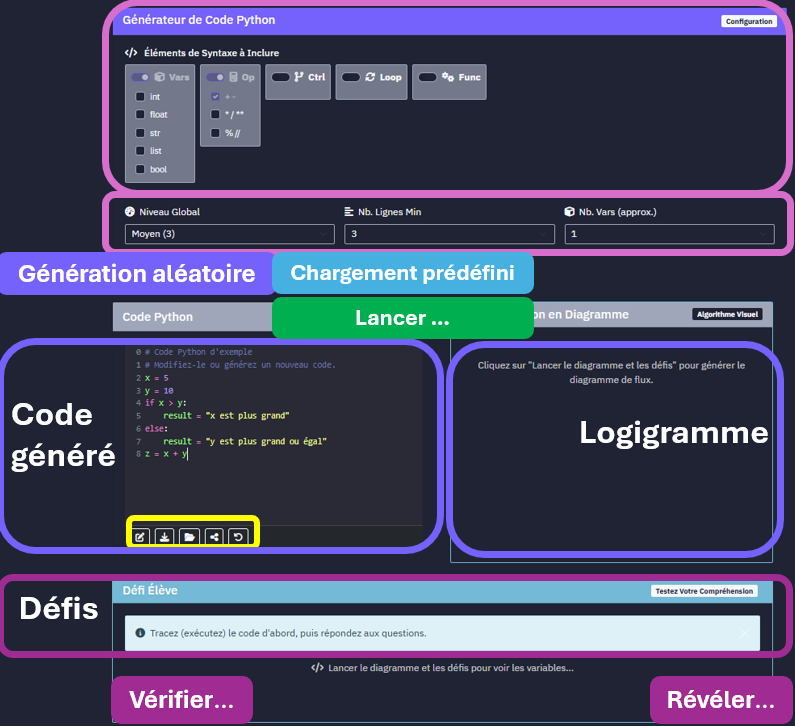
\includegraphics[width=0.99\textwidth, keepaspectratio]{UI_events_v2.png}
    \caption{Présentation générale de l'application, vierge}
    \label{fig:UI_events}
\end{figure}
Revoyons de façon plus schématique cette même architecture, avec mise en valeur des ``clicks'' par une flèche colorée, évoquant l'appel au serveur Flask et l'insertion en base de données (symbolisée par les disques magnétiques).
\begin{figure}[H]

    \centering
    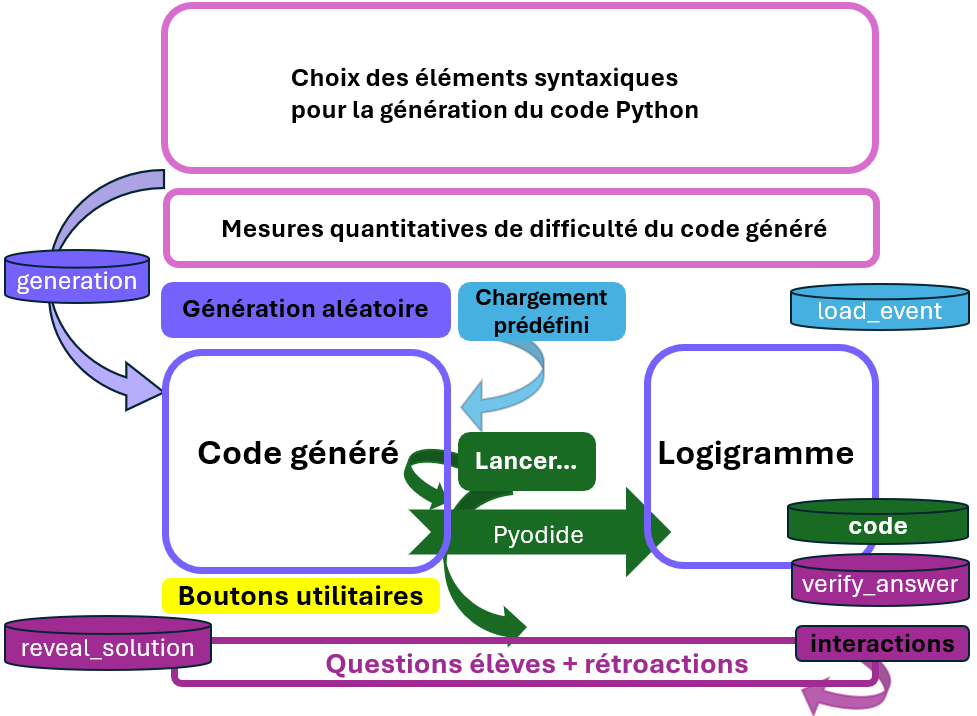
\includegraphics[width=0.8\textwidth, keepaspectratio]{simplif_archi.png}
    \caption{L'UI : événements journalisés}
    \label{fig:simplif_archi}
\end{figure}
Ce processus schématique se traduit concrètement par la base de données relationnelles \code{GYMINF\_POC} donc le diagramme Entité-Relation est visualisé par la figure \ref{fig:ERD} ci-dessous.
\begin{landscape}
\begin{figure}

    \centering
    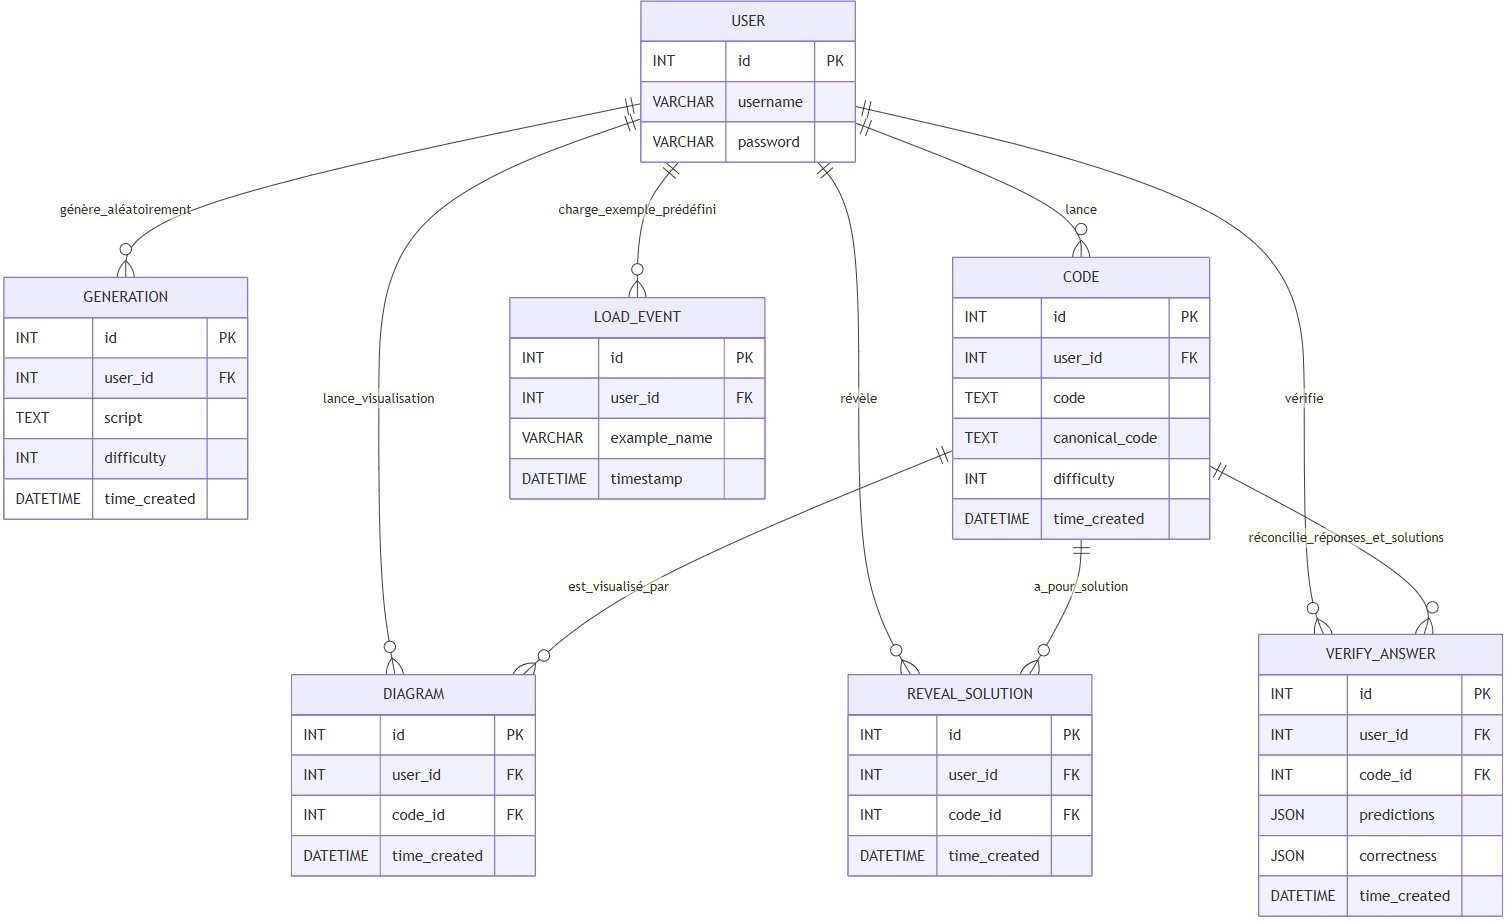
\includegraphics[width=1.5\textwidth]{erDiagram_logging.png}
    \caption{Diagramme Entité Relations complet de GYMINF\_POC}
    \label{fig:ERD}
\end{figure}
\end{landscape}

\subsection{Architecture et flux de journalisation}
Quel que soit l'événement, le processus de journalisation suit une architecture client-serveur tri-partite, comme illustré par la figure \ref{fig:logging_process_v3}.

\subsubsection{Description générale des étapes d'une journalisation}
Le flux débute par une action de l'utilisateur dans le \textbf{Navigateur (Front-end JS)}, qui est capturée par le code JavaScript. Ce dernier prépare une requête contenant les données pertinentes et l'envoie de manière asynchrone au \textbf{Serveur Web (Flask)}. Le serveur traite la requête, en appliquant d'abord la logique nécessaire (validation, authentification) et interagit avec la \textbf{Base de Données (SQL)} pour réaliser effectivement la journalisation par insertion des informations dans la table qui correspond au type d'événement sauvegardé. Enfin, le serveur renvoie une réponse au navigateur pour confirmer le succès de l'opération et, le cas échéant, transmettre des données en retour (comme un identifiant unique pour le défi en cours, qui servira pour le relier aux interactions ultérieures). \\Cette architecture garantit une séparation claire des responsabilités et en 
une interface utilisateur réactive : elle laisse toute la logique gérant l'expérience utilisateur dans le navigateur sans l'altérer par les contraintes liées à la journalisation, et fait intervenir le serveur uniquement comme une extension parallèle chargée de gérer la base de données.


\subsubsection{Types d'Événements Journalisés}
Le fichier \filepath{db\_queries.js} définit une énumération \code{log\_enum} qui liste les types d'événements pouvant être journalisés. Chaque type correspond à une route spécifique sur le serveur Flask.

\begin{itemize}
    \item \textbf{\code{GENERATION}:} Déclenché lors de la création d'un nouveau code Python via le générateur aléatoire.
    \item \textbf{\code{LOAD\_EXAMPLE}:} Déclenché lorsqu'un exemple de code prédéfini est chargé dans l'éditeur.
    \item \textbf{\code{FLOWCHART\_GENERATION}:} Déclenché lorsque l'utilisateur clique sur ``Lancer le diagramme et les défis'', ce qui implique la génération du diagramme et la préparation du défi. Cet événement enregistre à la fois le code original et sa version canonique (purgée par \code{ast.unparse(ast.parse()}).
    \item \textbf{\code{VERIFY\_ANSWERS}:} Déclenché lorsque l'élève soumet ses réponses au défi (les réponses peuvent être vides, l'élève a pu voir la solution du défi avant).
    \item \textbf{\code{REVEAL\_SOLUTION}:} Déclenché lorsque l'élève demande à voir la solution du défi (l'élève a pu soumettre ses réponses avant, ou non).
\end{itemize}
L'événement ``Vérifier les réponses'' se démarque des autres par l'insertion en base d'une structure de données plus sophistiquée, car il existe plusieurs réponses à donner à chaque exercice. Il s'agit donc de stocker le mapping entre chaque variable et la proposition de réponse correspondante proposée par l'élève, ainsi que le mapping entre le statut vrai/faux et la variable demandée. 

\begin{figure}[p]
\centering
\begin{adjustbox}{max width=\textwidth, max height=0.98\textheight, keepaspectratio, center}
\begin{tikzpicture}[
  node distance=1.0cm and 1.6cm,
  every node/.style={font=\normalsize},
]
% --- Styles de flèches unifiés ---
\tikzset{
  seq/.style  = {-Latex, ultra thick, draw=black},              % intra-lane
  call/.style = {-Latex, thick, dashed, draw=orange!85!black},  % interaction : appel
  ret/.style  = {-Latex, thick, dashed, draw=violet!85},        % interaction : retour
}

% =========================
% Lane 1 : Navigateur (Front-end JS) : main.js + db_queries.js
% =========================
\node[event] (start) {Action à logger};
\node[task, below=of start] (main_js) {\textbf{main.js}\\Appelle la fonction ad hoc};
\node[task, below=of main_js] (db_queries_prepare) {\textbf{db\_queries.js}\\Construit JSON};
\node[task, below=of db_queries_prepare] (db_queries_send) {\textbf{db\_queries.js}\\\code{logFactory(...)} \& \code{fetch()} (POST)};
\node[gateway, below=of db_queries_send, yshift=-0.2cm] (js_handle_response) {Réponse OK ?};
\node[task, below=of js_handle_response, yshift=-0.2cm] (js_success) {Traite la réponse (affichages)};
\node[event, below=of js_success] (end) {Log Terminé};
\node[task, right=of js_handle_response, xshift=0.2cm, yshift=0.8cm] (js_error) {Console.Log Error};

% =========================
% Lane 2 : Serveur Web (Flask) — remontée et rapprochée
% =========================
\node[task, right=of db_queries_send, xshift=5.2cm, yshift=8mm] (flask_route) {\textbf{app.py (Route)}\\\footnotesize \texttt{/log/...}};
\node[task, below=of flask_route] (flask_logic) {\textbf{app.py (Logique)}\\Valide données \& appelle BDD};
\node[data, below=of flask_logic] (json_response) {Réponse JSON (\code{status}, \code{id})};

% =========================
% Lane 3 : Base de Données (SQL) — remontée et rapprochée
% =========================
\node[data, right=of flask_logic, xshift=2.5cm, yshift=8mm] (sql_query) {Requête SQL\\(\code{INSERT}/\code{SELECT})};
\node[task, below=of sql_query] (db_execute) {\textbf{Serveur SQL}\\Exécute \& renvoie résultat};

% ============
% Flèches
% ============
% Intra-lane (seq)
\draw[seq] (start) -- (main_js);
\draw[seq] (main_js) -- node[midway, right, font=\scriptsize] {prépare données} (db_queries_prepare);
\draw[seq] (db_queries_prepare) -- node[midway, right, font=\scriptsize] {\code{logFactory()}} (db_queries_send);
\draw[seq] (flask_route) -- (flask_logic);
\draw[seq] (flask_logic) -- node[midway, right, font=\scriptsize] {construit} (json_response);
\draw[seq] (js_handle_response) -- node[midway, right] {Oui} (js_success);
\draw[seq] (js_handle_response) -- node[midway, above] {Non} (js_error);
\draw[seq] (js_success) -- (end);
\draw[seq] (js_error) -- (end);

% Interactions (call / ret)
\draw[call] (db_queries_send) -- node[midway, above] {HTTP POST} (flask_route);
\draw[call] (flask_logic) -- node[midway, above, font=\scriptsize] {envoie requête} (sql_query);
\draw[ret]  (db_execute) -- node[midway, right, font=\scriptsize] {résultat} (flask_logic);
\draw[ret]  (json_response) -- node[midway, above] {HTTP Response} (js_handle_response);

% ============
% Lanes + barres de titre (top/bottom communs), centrées autour des nœuds
% ============
% Pré-pad haut global pour dégager les bandeaux
\path[draw=none] ([yshift=12mm]start.north west) rectangle ([yshift=12mm]sql_query.east);

\begin{scope}[on background layer]
  % Groupes "fit" par lane (sans pads latéraux artificiels)
  \node[fit=(start)(main_js)(db_queries_prepare)(db_queries_send)
            (js_handle_response)(js_success)(end)(js_error),
        inner sep=10pt] (lane1_fit) {};
  \node[fit=(flask_route)(flask_logic)(json_response),
        inner sep=12pt] (lane2_fit) {};
  \node[fit=(sql_query)(db_execute),
        inner sep=12pt] (lane3_fit) {};

  % Bordures communes
  \coordinate (top)    at (current bounding box.north);
  \coordinate (bottom) at (current bounding box.south);

  % Paramètres
  \def\titlebar{12mm}
  \def\laneGap{8mm}   % écart horizontal entre lanes
  \def\padLR{10mm}    % padding latéral symétrique contenu↔bord

  % --- Lane 1 ---
  \coordinate (l1_wt) at (lane1_fit.west |- top);
  \coordinate (l1_et) at (lane1_fit.east |- top);
  \coordinate (l1_eb) at (lane1_fit.east |- bottom);
  \filldraw[fill=blue!5, draw=black, rounded corners]
    (l1_wt) rectangle (l1_eb);
  \fill[blue!30] (l1_wt) rectangle ([yshift=-\titlebar]l1_et);
  \node[anchor=west, font=\bfseries\normalsize]
    at ([xshift=2mm,yshift=-2.5\titlebar]l1_wt) {Navigateur (Front-end JS)};

  % --- Lane 2 : à droite de la lane 1 + gap ; largeur = (contenu) + padLR
  \coordinate (l2_wt) at ($(l1_et) + (\laneGap,0)$);
  \coordinate (l2_et) at ($(lane2_fit.east |- top) + (\padLR,0)$);
  \coordinate (l2_eb) at (l2_et |- bottom);
  \filldraw[fill=orange!5, draw=black, rounded corners]
    (l2_wt) rectangle (l2_eb);
  \fill[orange!30] (l2_wt) rectangle ([yshift=-\titlebar]l2_et);
  \node[anchor=west, font=\bfseries\normalsize]
    at ([xshift=2mm,yshift=-2.5\titlebar]l2_wt) {Serveur Web (Flask)};

  % --- Lane 3 : à droite de la lane 2 + gap ; largeur = (contenu) + padLR
  \coordinate (l3_wt) at ($(l2_et) + (\laneGap,0)$);
  \coordinate (l3_et) at ($(lane3_fit.east |- top) + (\padLR,0)$);
  \coordinate (l3_eb) at (l3_et |- bottom);
  \filldraw[fill=red!5, draw=black, rounded corners]
    (l3_wt) rectangle (l3_eb);
  \fill[red!30] (l3_wt) rectangle ([yshift=-\titlebar]l3_et);
  \node[anchor=west, font=\bfseries\normalsize]
    at ([xshift=2mm,yshift=-2.5\titlebar]l3_wt) {Base de Données (SQL)};
\end{scope}

% ============
% Légende en bas à droite (plus basse pour éviter tout chevauchement)
% ============
\begin{scope}
  \coordinate (legendSE) at ($(current bounding box.south east)+(-1.2cm,0.4cm)$);
  \node[draw, rounded corners, fill=gray!5, inner sep=4mm, anchor=south east] (legend) at (legendSE) {
    \begin{tikzpicture}[baseline]
      \draw[seq]  (0,0)--(1.6,0);      \node[anchor=west] at (1.8,0)       {\footnotesize Flux intra-participant};
      \draw[call] (0,-0.7)--(1.6,-0.7);\node[anchor=west] at (1.8,-0.7)    {\footnotesize Interaction — Appel (HTTP/SQL)};
      \draw[ret]  (0,-1.4)--(1.6,-1.4);\node[anchor=west] at (1.8,-1.4)    {\footnotesize Interaction — Retour (HTTP/SQL)};
    \end{tikzpicture}
  };
\end{scope}

\end{tikzpicture}
\end{adjustbox}
\caption{Diagramme BPMN du flux de journalisation des actions utilisateur}
\label{fig:logging_process_v3}
\end{figure}
%#######################################################

\subsection{Description détaillée des étapes : scénario d'un lancement de logigramme et de défi}

Le processus est similaire pour tous les types d'événements. Pour illustrer concrètement ce processus, considérons le scénario suivant : un élève (identifié par \code{user\_id=1}) décide de ``lancer le diagramme et le défi'' pour le code Python présent dans son éditeur. Pour rappel, ce bouton lance côté client la création du logigramme et de la section défi (par Pyodide).  Cet événement provoquera côté serveur l'action  de journalisation (appelée \code{FLOWCHART\_GENERATION} dans l'énumération, cf. \code{db\_queries.js}). Cet événement a été choisi car il a une sophistication supplémentaire qui est de retourner le code\_id, qui est une donnée cruciale car c'est la clé étrangère pour les relations ``Vérifier les réponses'' et ``Révéler la solution'', tandis que les autres événements se contentent d'une confirmation (statut succès/échec et le message éventuel correspondant). Le fait que le code a peut-être été modifié manuellement par l'élève après sa génération est capturé par une logique en amont côté client (voir explication ci-dessous).

\subsubsection*{Étape 1 : Le contexte côté client}
Au moment du clic, le code visible dans l'éditeur sera appelé \textbf{code courant} car il a plusieurs origines possibles (génération aléatoire ou chargement prédéfini) et a peut être subi des modifications par l'utilisateur. \\
Dans notre scénario, reprenons un code déjà évoqué plus haut, résultant d'une génération aléatoire, dont le niveau de difficulté s'établit à 3 (variable \code{difficulty}). L'élève a marqué des commentaires dans son code, pour s'aider dans l'exercice ou mémoriser la théorie, et il en résulte le code courant suivant :
\begin{minted}[fontsize=\small]{python}
# code avec modif
enabled = True  # affectation, bool
y = 1           # type int
def build(flag):
    output = not flag
    return output
# appel de fonction avec paramètre:
found = build(enabled) 
# affichage :
print("Le résultat de " + "build" + "(" + str(enabled) + ")" + " est " + str(found))
\end{minted}

Au moment où l'utilisateur clique sur le bouton "Lancer le diagramme et les défis" le processus est déclenché (cf. fichier: \filepath{main.js}, ligne n°1395.)  et la variable \code{originalCode} reçoit le code dans l'instance CodeMirror.\\
Le front-end va d'abord envoyer ce code à Pyodide pour analyse. Notre module \code{MyCFG.py} le normalise en retirant les commentaires et donc en standardisant le formatage. Il en résulte un code qui fait abstraction des marques cosmétiques du point de vue du Control Flow Graph de l'interpréteur et que nous appelons donc le \textbf{code canonique} :
\begin{minted}[fontsize=\small]{python}
enabled = True
y = 1

def build(flag):
    output = not flag
    return output
found = build(enabled)
print('Le résultat de ' + 'build' + '(' + str(enabled) + ')' + ' est ' + str(found))
\end{minted}
A ce stade, après résolution de la promesse Pyodide le front-end dispose du code courant, du code canonique et du niveau de difficulté.

\subsubsection*{Étape 2 : préparation et envoi de la requête AJAX}
Le gestionnaire d'événement dans \filepath{main.js} appelle la fonction asynchrone \code{logExecutedCode} (ligne n°1441) avec ces deux versions du code et la difficulté.\\
Dans \filepath{db\_queries.js} (ligne n°79) la fonction \code{logExecutedCode} prépare le corps (\code{body}) de la requête au format JSON et appelle ensuite la fonction centrale \code{logFactory} (ligne n°84) avec le type d'événement (ici \code{log\_enum.FLOWCHART\_GENERATION}) et son corps de requête.\\
Enfin la fonction \code{logFactory} (ligne n°159) utilise l'API \code{fetch} pour envoyer la requête \code{POST} asynchrone à la route Flask qui correspondant au type d'événement journalisé, c'est-à-dire à l'URL .
envoie la requête \code{POST} suivante à l'URL \code{/log/flowchart\_generation}. En suivant notre scénario la requête sera : 
\begin{minted}[fontsize=\small]{json}
{
  "code": "# code avec modif\nenabled = True\n...",
  "canonical_code": "enabled = True\ny = 1\n\ndef build(flag):\n...",
  "difficulty": 3
}
\end{minted}

\subsubsection*{Étape 3 : Routage puis traitement côté serveur de la requête et interaction avec la base de données}
Le serveur Flask reçoit la requête et la dirige vers la fonction Python associée (cf. \filepath{app.py}, ligne n°126 ). \\ 
Cette fonction de route \code{flowchart\_generation\_log\_route} extrait les données et l'identifiant de l'utilisateur de la session pour valider les données reçues et appeler la fonction de logique de base de données ici \code{executed\_code\_log} (cf. \filepath{app.py}, lignes n°127-148) qui obtient une instance de curseur de la connexion mySQL et exécute la requête SQL suivante (\filepath{app.py}, lignes n°323-339) :
\begin{minted}[fontsize=\small]{sql}
INSERT INTO code (user_id, code, canonical_code, difficulty, time_created) 
VALUES (1, 
        '# code avec modif...\n...', 
        'enabled = True\ny = 1\n...', 
        3, 
        NOW());
\end{minted}

La fonction valide ensuite la transaction par la commande \code{commit()} et retourne le nouvel identifiant du code journalisé (propriété \code{lastrowid} du curseur), pour finalement refermer explicitement le curseur - bonne pratique d'optimisation, voire de sécurité, pour les serveurs.

\subsubsection*{Étape 4 : La réponse HTTP et la mise à jour du client}
Supposons que la base de données a assigné l'\code{id=42} à cette nouvelle entrée. Le serveur Flask renvoie une réponse HTTP avec un statut 200 (OK) et le corps JSON suivant (cf. \filepath{app.py}, lignes n°138-148):
\begin{minted}[fontsize=\small]{json}
{
  "status": "success",
  "message": "Code exécuté et diagramme journalisés.",
  "code_id": 42
}
\end{minted}
 La promesse \code{fetch} dans \filepath{db\_queries.js} se résout : les blocs \code{.then()} de la fonction \code{logFactory} retournent les réponses JSON du serveur (\filepath{db\_queries.js}, lignes n°155-190). Les valeurs de retour sont remontées jusqu'à l'appelant, c'est-à-dire au code JavaScript (cf. \filepath{main.js} lignes n°1438-1444) qui stocke alors la valeur \code{42} dans la variable globale \code{currentChallengeCodeId}.\\
 Désormais, toute interaction ultérieure de l'élève avec ce défi (vérification ou révélation de la solution) sera liée à l'entrée \code{code\_id=42} dans la base de données, assurant une traçabilité complète de l'exercice. Si l'élève modifie ensuite le code de façon superficielle (par exemple, en éditant ses commentaires) la référence est conservée. Si la modification est sémantique alors l'interface se grise pour obliger à ``(re)lancer le diagramme et les défis''. 



\clearpage
\begin{minipage}{\textwidth}
    
\subsection{Visualisation logique et exhaustive de la journalisation}
Revoici la schématisation utilisée précédemment, ajoutant en regard des événements les noms de chaque table et des attributs écrits dedans.
\begin{figure}[H]
    \centering
    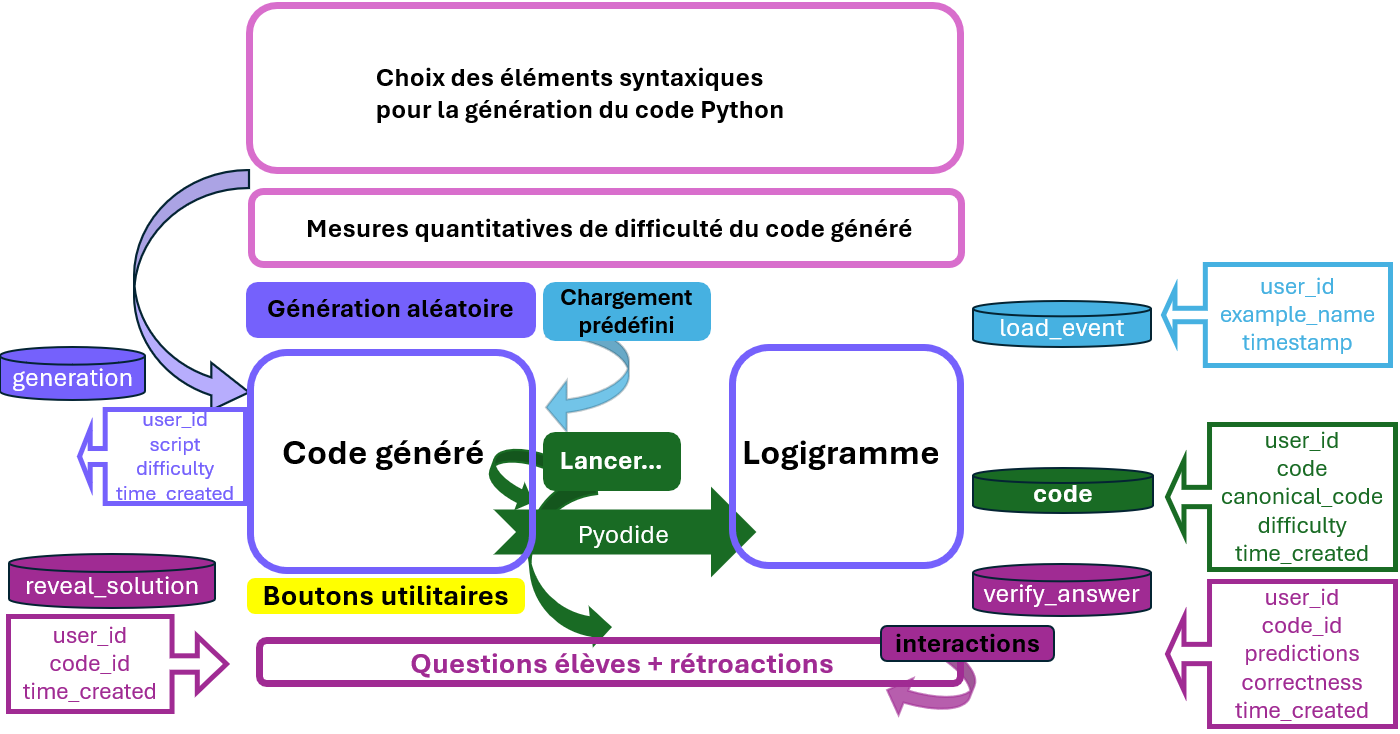
\includegraphics[width=0.99\textwidth, keepaspectratio]{logging_archi.png}
    \caption{Présentation générale de l'application, vierge}
    \label{fig:logging_archi}
\end{figure}
Pour une présentation exhaustive des écritures, toutes déjà implémentées mais non encore utilisées dans un dispositif en classe, voici un tableau situant chaque événement dans son processus ``Front-end $\rightarrow$ (Flask $\Leftrightarrow$ SQL) $\rightarrow$ Front-end'' utilisant le même code couleur que ci-dessus.
\begin{figure}[H]

    \centering
    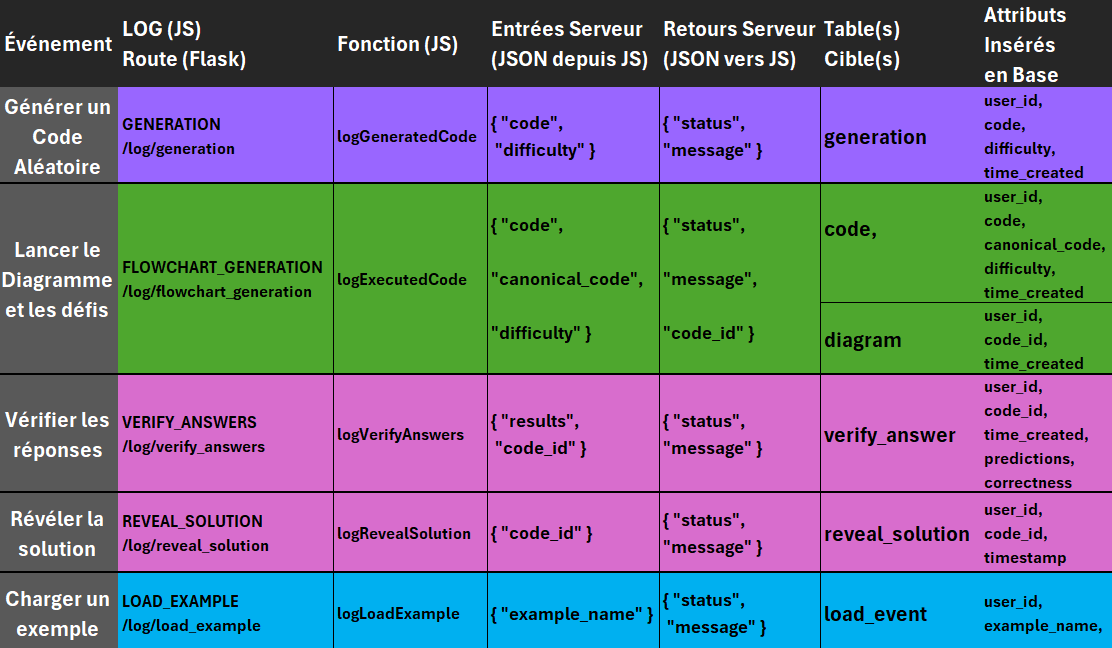
\includegraphics[width=0.99\textwidth, keepaspectratio]{tableau_journalisations.png}
    \caption{L'UI : événements journalisés}
    \label{fig:tableau_journalisations}
\end{figure}

\end{minipage}


\clearpage
\subsection{Défis techniques et solutions implémentées}

La conception d'un environnement d'apprentissage interactif et instrumenté comme le nôtre soulève plusieurs défis techniques. Notre architecture actuelle est le fruit de solutions pragmatiques répondant à des contraintes spécifiques de performance, de logique pédagogique et de robustesse des données.\\ Cette approche "Problème-Solution" a guidé le développement de notre système de journalisation et d'analyse de code.
\begin{table}[htbp]
    \centering
    \caption{Tableau de correspondance entre les défis techniques et les solutions implémentées}
    \label{tab:challenges-solutions} 
    % \textwidth signifie que le tableau occupera toute la largeur du texte.
    % La première colonne 'l' est alignée à gauche et prend sa largeur naturelle.
    % Les deux colonnes 'X' sont des colonnes spéciales de tabularx.
    % Elles sont justifiées et se partagent l'espace restant de manière égale.
    \begin{tabularx}{\textwidth}{@{} l X X @{}}
        \toprule
        \textbf{N°} & \textbf{Défi Technique} & \textbf{Solution Architecturale Implémentée} \\
        \midrule
        
        1 & \textbf{Suivi Pédagogique Individuel.}
            Comment lier de manière fiable chaque action de l'élève (génération, vérification, etc.) à son profil et à un exercice précis ?
            & \textbf{Journalisation Authentifiée et Contextualisée.}
            Chaque requête AJAX est authentifiée via la \textbf{session Flask}. Une création d'utilisateur génère un \textbf{\code{user\_id}}, une génération d'exercice génère un \textbf{\code{id}} unique. Ces ID pourront ensuite être utilisées pour lier toutes les interactions ultérieures (à travers les tables de la base de données), garantissant un suivi cohérent. \\
        \addlinespace

        2 & \textbf{Dualité du Code Source.}
            Comment gérer et journaliser à la fois le code initialement chargé et le code potentiellement modifié par l'élève dans l'éditeur ?
            & \textbf{Double Capture et Restauration.}
            Un code généré ou chargé peut être modifié dans l'éditeur. La variable JS \code{lastLoadedCode} sert de point de restauration pour l'élève. Lors de la journalisation, nous enregistrons systématiquement deux versions : le \textbf{code original} (brut, de l'éditeur) et sa \textbf{version canonique} (via \code{ast.unparse}). Cela offrira la possibilité d'analyses fines des modifications de l'élève, et ouvrira même la possible constitution de \textit{big data} sur les interactions élèves. \\
        \addlinespace

        3 & \textbf{Variations Cosmétiques vs. Changements Structurels.}
            Comment éviter de journaliser un nouvel exercice si l'élève n'a fait que des changements non-logiques (commentaires, espaces) ?
            & \textbf{Détection de Doublons via le Code Canonique.}
            La version canonique du code sert d'``empreinte digitale'' de sa structure. Une variable JS, \code{lastLoggedCanonicalCode}, mémorise la dernière empreinte journalisée. Un nouvel enregistrement n'est effectué que si la nouvelle empreinte est différente, évitant ainsi les doublons logiques. \\
        \addlinespace

        4 & \textbf{Latence de l'Analyse Côté Client.}
            Comment minimiser la lenteur perçue par l'utilisateur due aux multiples appels asynchrones (\code{await}) nécessaires à Pyodide pour analyser le code ?
            & \textbf{Appel Unifié à Pyodide.}
            Au lieu de multiples appels \code{await} pour chaque artefact, une méthode centrale en Python, \code{process\_and\_get\_results()}, est appelée une seule fois. Elle orchestre en une passe le parsing, la construction du graphe, et la génération de tous les artefacts nécessaires (\code{mermaid}, \code{canonicalCode}, \code{ast\_dump}), qui sont retournés dans un unique objet. \\
        
        \bottomrule
    \end{tabularx}
\end{table}


\clearpage
\section{Travaux futurs, discussions et conclusions}
 Certaines limitations sont connues et nous en ferons une liste ci-dessous. Certaines sont en cours de résolution. Aussi, dans l'attente de voir l'outil utilisé en classe, nous pouvons indiquer dans quelles directions notre outil semble orienter de prochaines recherches.

\subsection{Des orientations de recherche qui pourraient être soutenues par notre outil}
\subsubsection{La question des indicateurs pertinents}
La possibilité de confronter des élèves à des difficultés que l'on peut caractériser quantitativement (nombre de structures syntaxiques différentes, longueur du code, nombre de variables) et qualitativement (types de variables, types de structures) tout en mesurant les performances des élèves(réussite/échec sur chaque variable) amène naturellement à se poser la question de la construction d'indicateurs pertinents.

\subsubsection{Des questions épistémologiques rendues empiriques}
Dans quelle mesure :\begin{itemize}
    \item L'apport de la visualisation graphique améliore-t-elle l'apprentissage de la programmation Python chez les débutants ?
    \item La génération aléatoire de code contrôlée par objectifs soutient-elle l'apprentissage chez les débutants dans le cadre de l'approche PRIMM ?
    \item La mise à disposition de l'outil, avec sa capacité de génération infinie et sa rétroaction automatique non bloquante, a-t-elle un effet sur la rétention à long terme des élèves ?

\end{itemize}


\subsection{Des idées abandonnées par manque de temps}
\begin{enumerate}
    \item Contrôler l'aléa en utilisant un ensemble de \textit{templates} à remplir pour chaque classe d'exercices à générer (plutôt qu'une approche grammaticale du langage) $\Rightarrow$ Idée alternative pour faire d'un script un véritable exercice: prédéfinir les questions à poser aux élèves selon le \textit{template} choisi (\textit{aka} la classe d'exercices)\par Exemples: "Quel est le nombre de passages dans la boucle?" si une boucle est choisie, "Combien de fois le bloc $xyz$ a-t-il été exécuté?" si des boucles imbriquées ont été choisies, etc. 
    
    \item Générer les valeurs attendues simultanément aux \textit{erreurs attendues} signifiantes afin de pouvoir fournir un feedback à valeur ajoutée $\Rightarrow$ Idée plus radicale: se limiter à des affectations de valeurs (les questions aux élèves se limiteraient à "Valeur de x = ...", "valeur de y = ...")

    \item Préparer des questions "Comment serait modifiée la valeur si ... \textit{(ici la modification à prévoir)} ?" en plus, pour renforcer/tester la compréhension.
    
    \item Ouvrir la possibilité de générer un script invalide \textbf{exprès} comme variable didactique $\Rightarrow$ besoin de contrôler quelles sont les erreurs permises (Division par zéro? Index Error? etc.) 
    
    \item La génération d'exercices "Chercher l'erreur", y compris erreurs sémantiques et/ou syntaxiques? Un intérêt pédagogique avéré (le débogage) mais secondaire par rapport à mes objectifs curriculaires.
\end{enumerate}


\subsection{Travaux pour améliorer l'approche actuelle}
Les améliorations envisagées sont d'ordre quantitatif (ajouts d'éléments) et qualitatif.

\begin{itemize}
    \item Enrichir les types d'exercices et la section "Défis": 
    \begin{enumerate}
        \item Proposer une option "Debug" qui génère des codes invalides, avec des boucles infinies ou syntaxiquement incorrects, appelant les élèves à identifier les erreurs selon leur type.
        \item Des questions qualitatives qui peuvent être ouvertes ou fermées par menu déroulant : Quels sont les types des variables ? (les types étant à récupérer depuis le générateur de code).
        \item Des questions quantitatives \textit{in situ} : Combien de passages dans la boucle ? Combien de passages à tel point du code ?
        \item Des questions mobilisant des concepts théoriques : Telle boucle du code est-elle bornée ? 
    \end{enumerate}

    \item Proposer des QCM sur le code généré, avec erreurs attendues mélangées avec la bonne réponse et des erreurs totalement \textit{random}.
    
    \item Améliorer les rétroactions pour le bouton "Vérifier":
    \begin{enumerate}
        \item Utiliser la réponse élève pour l'analyser au regard des erreurs attendues pour donner des indices (cf. litérature didactique)
        \item Ajouter des \textit{tooltips} (visibles en survolant l'espace de réponse avec le pointeur souris) pour donner des indications de réponses ou des bonnes questions à se poser, pour baliser le travail des élèves
    \end{enumerate}
    
    \item Améliorer l'interface pour renforcer l'engagement :
    \begin{enumerate}
        \item Rendre le \textit{flowchart} cliquable pour un meilleur rendu smartphone
        \item Améliorer la \textit{responsiveness}, notamment les espaces horisontaux pris par les cartes en haut de page
        \item Utiliser des "combines addictives" pour faire revenir les utilisateurs
    \end{enumerate}


    \item Améliorer le rendu \textit{flowchart}:
    \begin{itemize}
    
    \item Éléments syntaxiques Python à implémenter : 
    \begin{enumerate}
        \item le \textit{break} à connecter au nœud terminal de sa boucle
        \item les \code{try: except: else: finally:}, les \code{Raise}, les \code{Assert}, ...
        \item Un traitement des annotations de type ?
        \item un traitement de la récursion ?
    \end{enumerate}
    
    \item numéroter les nœuds graphique selon \texttt{lineno} pour visualiser correspondance syntaxe $\Leftrightarrow$ sémantique
    
    \item colorer les flèches "True / False" resp. Bleu/Rouge
    
    \item clarifier (coloriser?) les rendus graphiques des différents types d'appels: internal\_call, appels de type I/O, ...

    \item animer les éléments graphique pour réduire la charge cognitive de l'élève ?
    \end{itemize}
    
\end{itemize}

\subsection{ Des réponses aux critiques les plus probables}
Les objections qui pourraient être faites: expliciter des choix assumés, notes des limitations actuelles dont les solutions ont déjà été pensées et non encore implémentées, des approches alternatives (en cours de recherche ou à l'état complètement hypothétique)

\subsubsection*{Critique sur la finalité des codes générés proposés aux élèves}
Deux reproches pourraient nous être faits à ce titre:
\begin{itemize}
    \item Le code généré manque de "sens" ou d'intentionnalité. Il ressemble à une suite d'opérations aléatoires plutôt qu'à un algorithme résolvant un problème.
    \item La génération basée sur des motifs et listes de noms de variables prédéfinis limite la créativité et ne prépare pas les élèves à la résolution de problèmes authentiques.
\end{itemize}
Ces critiques sont valides et sont le résultat d'un compromis assumé. L'outil se positionne au début du spectre de l'apprentissage, correspondant aux phases "Predict" et "Run" du modèle PRIMM. À ce stade, la familiarisation avec des motifs standards et des noms de variables conventionnels (\texttt{i}, \texttt{count}, \texttt{items}) est un objectif pédagogique en soi. La créativité et la résolution de problèmes authentiques interviennent dans les phases ultérieures. Nous pensons que notre outil est de nature à supporter les stades "Investigate" et "Modify" en permettant à l'élève de modifier librement le code généré. Le générateur fournit donc un "échafaudage" sur lequel l'élève peut ensuite construire, et un outil qui décharge du temps pour l'enseignant. L'objectif de l'outil n'est pas de générer des solutions à des problèmes complexes, mais de fournir des extraits de code ciblés pour l'apprentissage de la syntaxe. Les fonctions chooseAppropriateParameterNames et generateStructureBody sont des tentatives pour injecter une plausibilité sémantique dans notre approche aléatoire et impérative, mais l'objectif principal reste la maîtrise des constructions du langage, pas la conception algorithmique.

\subsubsection*{Critique sur l'approche impérative et aléatoire de génération de code}
A la suite de la critique précédente, il vient l'observation qu'une autre approche aurait pu être plus élégante sur le plan théorique et pour l'implémentation, comme une approche déclarative, par solveur de contraintes par exemple, ou par modèles de langage. \\ 
Nous avons déjà répondu en préambule à la question de la délégation de la solution à une API du commerce ou un modèle propriétaire. Nous répondons ici que le déploiement d'une solution JavaScript s'exécutant dans le navigateur pare aux problèmes logistiques de déploiement d'une solution plus lourde. Ajoutons enfin que que notre approche impérative actuelle avec ses phases (préparation, écriture et vérification) est très verbeuse mais relativement performante et déterministe dans son comportement, qui peut être déboguée avec nos outils standards. C'est un choix pragmatique privilégiant la faisabilité et la performance dans le temps imparti et le contexte technologique imposé.


\subsection{Travaux pour une nouvelle approche de génération de code}

\subsubsection*{Approche par ``template sémantique''}
Un pré-requis pour cette approche est de disposer d'une base de codes ``organiques'' ayant un sens et résolvant un problème, de différents niveaux, toujours compatibles avec nos objectifs poursuivis : l'enseignement auprès des débutants d'école secondaire. Il serait alors possible par analyse systématique des AST de caractériser chaque code finement (selon les éléments syntaxiques utilisés) et il sera ensuite possible d'\textit{aléatoiriser} chaque code, en substituant aux variables didactiques (noms et valeurs affectées aux variables) d'autres, en accord avec les objectifs pédagogiques sélectionnés par l'utilisateur.

\subsubsection*{A quoi ressemblerait une approche déclarative}
On ne ferait que décrire le résultat final. Le système se chargerait de trouver un code qui respecte cette description:
 
 \begin{minted}{javascript}
const codeDescription = {
    targetLines: 20,
    difficulty: 3,
    mustContain: ['if', 'for_list'],
    mustUseVariables: ['int', 'list'],
    allVariablesMustBeUsed: true,
    noInfiniteLoops: true
};
const generatedCode = declarativeGenerator.generate(codeDescription);
\end{minted}

\subsubsection*{A quoi ressemblerait une approche par solveur de contraintes}
La génération de code pourrait être modélisée comme un problème de contraintes :

Les variables :
\begin{itemize}
    \item chaque ligne de code potentielle, 
    \item chaque nom de variable, 
    \item chaque valeur littérale.
\end{itemize}

Les contraintes : 
\begin{itemize}
    \item contrainte\_longueur : Le nombre total de lignes doit être entre 15 et 20.
    \item contrainte\_syntaxe : Si l'option if est cochée, le code doit contenir au moins un bloc if.
    \item contrainte\_dépendance : Si un bloc for..in..list existe, alors une variable de type list doit exister et être déclarée avant la boucle.
    \item contrainte\_unicité : Deux variables ne peuvent pas avoir le même nom.
    \item contrainte\_utilisation : Chaque variable déclarée doit apparaître au moins une fois dans une expression après sa déclaration.
    \item contrainte\_terminaison : Le programme doit se terminer par une instruction de retour ou une sortie.
    \item contrainte\_sémantique : Les opérations doivent être logiques (ex: ne pas soustraire deux chaînes de caractères).
\end{itemize}
Le solveur de contraintes recevrait toutes ces règles et tenterait de ``construire'' un programme valide qui les respecte toutes.


------------------------------------------------------
\section*{Stack technologique: choix \& hypothèses}

\subsection*{UI}

\begin{enumerate}
    \item Chargement des dépendances (parmi tous les possbles pour exécuter du Python dans le navigateur, préférence = $Pyodide$, et en plus $Skulpt$ si besoin) $+$ la jungle des frameworks pour affichage "joli": gros travail de debugging à prévoir même avec $LABjs$
    
    \item Des \texttt{checkbox} pour choisir les \textit{templates}, avec une logique d'exclusion de choix mutuellement exclusifs à définir et à implémenter (si et seulement si la boucle $for$ est choisie il existe la possibilité d'imbriquer des boucles, autre exemple selon le niveau de difficulté choisie on peut griser ou rendre visible certains choix, etc.)
    
    \item Les deux vues  \texttt{script} dans un éditeur de code, et \texttt{flowchart} si implémentées: onglets ou $toggle$ entre les \texttt{<div>}.
    
    \item Pour la présentation du feedback élève à renvoyer après enregistrement des réponses élèves: coloration des cellules $+$ modales pour retours ad hoc, notamment selon comparaison avec erreurs attendues
    
    \item Une piste: les \texttt{tooltips}, pour ajouter des \texttt{mouseover} sur les tokens du code, si possibilité d'y avoir accès... Autre piste: à la création de l'arbre syntaxique, possibilité de récupérer les annotations des noeuds par les parseurs Python
\end{enumerate}

\subsection*{Pistes et Hypothèses spécifiques flowchart... desquelles dépendra la logique de génération du code!}

Des solutions très difficiles à créer from scratch, ou des solutions difficiles qui alourdissent la stack.

\begin{enumerate}
    \item Manipuler directement le DOM de l'UI via Pyodide: créer les éléments HTML appropriés et concevoir leur manipulation (= réinventer la roue, puisque des bibliothèques spécialisées ont été créées pour ça)... $\Rightarrow$ idées suivantes:
    \item Bibliothèques JS existantes, exemple $Mermaid.js$: il faut que Python communique le flowchart à Mermaid $\rightarrow$ d'où l'idée du parsing AST
    \item $Graphviz$ et son $DOT language$: à ma connaissance en WebAssembly (accessoirement alourdirait le chargement de la page) donc \textit{à ma connaissance} impossibilité de modifier le DOM directement rendant compliquée (impossible?) l'option du rendu dynamique du flowchart... MAJ 26/03/25 des modules Python existeraient pour faire le travail demandé: cf. \url{https://github.com/pydot/pydot}
\end{enumerate}

\subsection*{Génération du code - des idées de pistes avec une supposition à questionner sur le besoin de travailler l'AST correspondant}

Différentes approches à envisager, pas forcément mutuellement exclusives.

\begin{description}
    \item[Approche texte + \texttt{ast}:] Le générateur de code créerait le script à afficher (texte) par application de \textit{templates} préddéfinis en les remplissant au fur et à mesure avec les variables et structures sélectionnées aléatoirement (exemple: "\texttt{if <condition> : <indent> <bloc>}). Approche la plus accessible et la plus facile à controler pédagogiquement, et la plus intuitive pour la production du script car on travaille du texte (ce que l'on veut en sortie) mais il manque le lien logique pour nous rapprocher du flowchart: besoin d'analyser la syntaxe du code généré pour en extraire la structure du code! C'est ce que promettent des fonctions comme \texttt{ast.parse()} pour retourner la racine de l'arbre syntaxique, et la classe \texttt{ast.NodeVisitor} pour parcourir les noeuds intéressants à traduire en noeuds flowchart (pour en garder que les éléments ciblés par nos objetifs pédagogiques). Pyodide est sensé nous donner la possibilité de créer et manipuler les éléments HTML correspondants, à styliser avec une classe CSS correspondante (à définir... plus facile à dire qu'à faire: il faudra supporter l'ancienneté des navigateurs installés dans les écoles et les terminaux des élèves iOS v18 et plus...).
     
     \item[Approche naïve:] S'inspirer de \cite{fuzzingbook} qui semble choisir des productions grammaticales correctes, mais à la signification aléatoire. 

     \item [Approche AST radicale:] Générer un AST pour le traduire en Python et le traduire en flowchart = utiliser l'AST comme une sorte de DSL en faisant une application intensive du module \texttt{ast}. Approche inspirée de ce que j'ai compris de \url{https://github.com/radomirbosak/random-ast}. Utiliser l'arbre assurerait une cohérence syntaxique par rapport au langage (et permettrait des erreurs $Index Error$ ou $Division by zero$ et d'autres plus difficiles à contrôler). Le module \texttt{astor} semble faire le job de traduire l'arbre en code (cf. \url{https://pypi.org/project/astor/}). Le problème principal est la difficulté de créer le générateur d'arbre AST ! Sans parler de la difficulté de le maintenir pérenne selon les mises à jour Python !
     
    \item[Approche via DSL radicale:] D'après \url{https://en.wikipedia.org/wiki/Domain-specific_language} il s'agit d'une solution standard dans l'industrie logicielle de concevoir un DSL adapté à un problème spécifique afin de faciliter la génération de solutions... mais qui semble totalement hors de portée, dépassant le cadre de ce projet, à moins d'en trouver un clé en main !
    
\end{description}

\newpage


\newpage
\section{Annexes}

\subsection{Check-list de \textit{convivialité} au sens d'Illich pour un service numérique et invitation à la réflexion}
En français, d'après le \textit{Larousse} le mot ``convive'' a une signification ancienne : \begin{quote}
    Personne qui prend ou doit prendre part à un repas
\end{quote} qui a donné son sens au mot ``convivialité'' qui a - toujours d'après le \textit{Larousse} - deux significations aujourd'hui: \begin{quote}
\begin{enumerate}
    \item Capacité d'une société à favoriser la tolérance et les échanges réciproques des personnes et des groupes qui la composent.
    \item Facilité d'emploi d'un système informatique.
\end{enumerate}
\end{quote}
Ivan Illich a donné un sens particulier à ce mot dans les années 1970. Pour inciter les enseignants et leurs élèves à se questionner sur le sujet, nous vous proposons une \textit{check-list} pratique et facile à mettre en place, qui ne nécessite pas de faire appel aux auteurs originaux de philosophie politique et sociologie.
\par L'idée est d'attribuer une note entre 0 et 6 à chaque service numérique, par l'application de 6 critères, chacun évalué entre 0 et 100\% selon que la réponse à la question est totalement négative (0\%) ou parfaitement juste (100\%).
\begin{description}
    \item[Appropriation \& autonomie] L’usager peut-il apprendre, utiliser, réparer/modifier l’outil sans dépendre d’experts ou d’un prestataire unique ?
    \item[Auto-limitation \& échelle humaine] Le service fixe-t-il des limites à sa taille/complexité/effet réseau pour éviter la capture (l'addiction, la croissance illimitée, les dépendances opaques) ?
    \item[Gouvernance par les usagers] La communauté participe-t-elle réellement aux règles (statuts, votes, roadmap publique) ?
    \item[Transparence \& auditabilité] Code/algorithmes/logs sont-ils documentés, vérifiables (ou, a minima, explicables et audités) ?
    \item[Portabilité \& réversibilité] Export complet, formats ouverts, interopérabilité, pas de lock-in, migration/fork sont-ils tous et toujours permis ?
    \item[Sobriété \& lien social] L'outil favorise-t-il la coopération plutôt que la captation/compétition ? ou au contraire contraint-il l’usage des ressources (énergie, attention, données)
\end{description}

\textbf{Interprétation} : 5-6 = outil convivial ; ... <2 = logique de contrôle.


\subsection{Documentation technique}

\subsubsection{Documentation Technique du Générateur de code}
Cette section détaille le fonctionnement interne des fonctions principales du script \code{code-generator.js}. L'architecture repose sur un ensemble de fonctions orchestrées pour garantir la génération d'un code Python à la fois aléatoire, cohérent et pédagogiquement pertinent, en respectant scrupuleusement les options sélectionnées par l'utilisateur.

\subsubsection*{Schéma des appels de fonctions internes à l'exécution de la génération de code aléatoire}

%\textit{}:
% → : Alt + 26
% │ : Alt + 179
% └ : Alt + 192
% ├ : Alt + 195
% ─ : Alt + 196
%

\begin{verbatim}
├── code-generator.js
│   │
│   └── generateRandomPythonCode(options)
│       │
│       ├── 1. FONCTIONS UTILITAIRES & DE SUPPORT (*)
│       │   ├── safeIndent                                #1221
│       │   ├── shuffleArray                              #844
│       │   ├── getRandomInt, getRandomItem               #73, #81
│       │   ├── getValueRange                             #68
│       │   ├── generateValueForType, generateValueOfType #306, #347
│       │   ├── generateUniqueVarName, generateUniqueIteratorName #141, #89
│       │   ├── chooseAppropriateParameterNames           #1203
│       │   ├── getDefaultValueForType                    #1423
│       │   └── declareVariable                           #168
│       │
│       ├── 2. LOGIQUE DE GÉNÉRATION CENTRALE (appelée par autres fonctions)
│       │   ├── generateVariedOperation                   #1743 (logique anti-répétition incluse)
│       │   └── generateAppropriateStatement              #1225
│       │       └── generateVariedOperation*
│       │
│       ├── 3. PHASES D'EXÉCUTION (dans l'ordre d'appel)
│       │   │
│       │   ├── A. Phase de Préparation
│       │   │   ├── calculateRequiredLines                #1247
│       │   │   ├── generateInitialVariables              #366
│       │   │   ├── ensureVariablesForOptions             #1598
│       │   │   │   ├── ensureVariablesOfType             #1453
│       │   │   │   │   └── declareVariable*
│       │   │   │   └── ensureRequiredVariables           #1624
│       │   │   │       └── ensureVariableExists          #189
│       │   │   │           └── declareVariable*
│       │   │   ├── ensureListVariablesCount              #202
│       │   │   │   ├── generateDiverseList*
│       │   │   │   ├── declareVariable*
│       │   │   │   └── ensureListVariableIsUsed          #230
│       │   │   └── ensureTypeSpecificOperations          #1977
│       │   │       └── generateVariedOperation*
│       │   │
│       │   ├── B. Phase de Génération des Structures
│       │   │   └── generateControlStructures             #508
│       │   │       ├── shuffleArray*
│       │   │       ├── generateIfStatement               #848
│       │   │       │   ├── generateCondition
│       │   │       │   └── generateAppropriateStatement*
│       │   │       ├── generateForRangeLoop              #920
│       │   │       │   └── generateStructureBody
│       │   │       ├── generateForListLoop               #946
│       │   │       │   └── generateStructureBody
│       │   │       ├── generateForStrLoop                #986
│       │   │       │   └── generateStructureBody
│       │   │       ├── generateWhileLoop                 #1019
│       │   │       │   ├── generateCondition
│       │   │       │   └── generateStructureBody
│       │   │       └── generateFunction                  #1060
│       │   │           ├── chooseAppropriateParameterNames*
│       │   │           ├── generateStructureBody
│       │   │           └── ensureVariableExists*
│       │   │
│       │   ├── C. Phase de Finalisation
│       │   │   ├── ensureAllVariablesAreUsed             #1441
│       │   │   │   └── generateVariedOperation*
│       │   │   ├── addFiller (boucle de remplissage)     #1650
│       │   │   │   └── generateVariedOperation*
│       │   │   └── finalVariableCheck                    #1384
│       │   │       ├── declareVariable*
│       │   │       └── getDefaultValueForType*
│       │
│       └── ***LEGACY*** (finalVariableCheck a un rôle résiduel)
├── main.js
│   └── ... (logique de l'interface utilisateur, gestion des options)
│
└── MyCFG.py
    └── ... (logique d'analyse du code Python et de génération du diagramme)
\end{verbatim}

\begin{description}
\item[Portée:] Ces variables sont déclarées au niveau supérieur de la fonction \methodname{generateRandomPythonCode}. Grâce au mécanisme de clôture (closure) de JavaScript, elles sont accessibles et partagées par toutes les fonctions auxiliaires imbriquées, agissant comme un état centralisé et encapsulé pour une unique session de génération de code.
\item[Variables Clés:]
\begin{itemize}
\item \var{options}: \vartype{object}. Objet contenant toutes les options de configuration booléennes et numériques récupérées depuis l'interface HTML. C'est la source de vérité pour toutes les décisions de génération !
\item \var{codeLines}: \vartype{Array<string>}. Tableau servant d'accumulateur, chaque élément étant une ligne du code Python final. Le rôle des fonctions de génération est d'ajouter des lignes à ce tableau.
\item \var{declaredVarsByType}: \vartype{object}. Structure de données centrale qui catalogue les noms de toutes les variables déclarées, classées par type. Exemple: \code{{ int: ['count', 'x'], str: ['name'] }}.
\item \var{allDeclaredVarNames}: \vartype{Set<string>}. Ensemble stockant tous les noms de variables déjà utilisés. Sa nature de \textit{Set} garantit l'unicité.
\item \var{linesGenerated}: \vartype{number}. Compteur simple qui suit le nombre de lignes de code générées pour respecter la limite fixée par l'option \param{numLinesGlobal} qui définit l'objectif à atteindre \var{targetLines}: ni trop, ni trop peu.
\end{itemize}
\end{description}

\subsubsection*{Fonctions de Génération}

\begin{enumerate}
    \item \methodname{generateInitialVariables} \#366
    \begin{description}
        \item[Signature:] \code{() -> \rettype{void}}
        \item[Description:] Initialise le script en créant les variables explicitement demandées par l'utilisateur via les options \param{var\_...\_count}. Ajoute à la liste \var{typesToGenerate} les types et la quantité correspondante \code{"type : count"} reçus de HTML ; Parcourt \var{typesToGenerate} jusqu'à atteindre la taille demandée (le nombre de variables "count") ; Génère un nom et une valeur selon le type, par appels à \code{generateUniqueVarName} et \code{generateValueForType} ; Ajoute l'initialisation aux lignes de code Python générées ; Met à jour les catalogues centralisés des variables déclarées \var{allDeclaredVarNames} et \var{declaredVarsByType}, et le compteur linesGenerated. Une boucle de sécurité répète tant que les nombres de variables et de lignes de code n'ont pas tous les deux atteints les tailles demandées. La condition de sécurité est exactement: \code{while (allDeclaredVarNames.size $<$ Math.min(MAX\_TOTAL\_VARIABLES, options.numTotalVariablesGlobal $||$ 3) \&\& linesGenerated $<$ targetLines)}
    \end{description}

    \item \methodname{generateUniqueVarName(type)} \#141
    \begin{itemize}
        \item Renvoie un nom de variable qui n'a pas encore été utilisé, parmi l'ensemble prédéfini, pour le type passé en argument
        \item Construit un tableau des noms disponibles pour ce type, puis filtre ce tableau de noms en ne gardant que les noms qui n'ont pas encore été déclarés (c'est-à-dire qui ne sont pas présents dans le Set allDeclaredVarNames), et renvoie un nom choisi au hasard parmi ceux filtrés
        \item Si tous les noms sont pris pour ce type, en crée un nouveau par ajout de suffixe numérique
    \end{itemize} 

    \item \methodname{generateValueForType} \#306
\begin{description}
    \item[Signature:] \code{(\param{type}: \vartype{string}) -> \rettype{string | number | boolean}}
    \item[Description:] Agit comme un simple dispatcher pour obtenir une valeur littérale. Il utilise le dictionnaire \code{LITERALS\_BY\_TYPE} qui associe chaque type à une \jsfunc{fonction anonyme} génératrice de valeur.
    \textit{Note d'implémentation :} Les \jsfunc{fonctions} de ce dictionnaire capturent la variable \var{difficulty} depuis la portée parente, centralisant ainsi la gestion du niveau de complexité des valeurs générées.
\end{description} 
    
    \item \texttt{ensureVariablesForOptions} \#1598
    \begin{itemize}
        \item Pour chaque type parmi int, float, str, list, bool: si le compteur est strictement positif, alors appeler \texttt{ensureVariablesOfType} avec en paramètres le type et le compteur 
        \item Appelle \texttt{ensureRequiredVariables}
    \end{itemize}

    \item \texttt{ensureVariablesOfType} \#1453
    \begin{itemize}
        \item Idem \texttt{generateInitialVariables}, en version générique pour tout choix des arguments type et count
    \end{itemize}

    \item \texttt{ensureRequiredVariables} \#1624
    \begin{itemize}
        \item Fonction de sécurité pour gérer le cas particulier des loop\_for\_list et loop\_for\_str et cond\_if sans que les types correspondants n'aient été choisis dans l'interface
        \item Dans ces cas: appelle \texttt{ensureVariableExists} avec le type en paramètre
    \end{itemize}

    \item \texttt{ensureVariableExists(type) } \#189
    \begin{itemize}
        \item Pour le type passé en paramètre, renvoie soit un nom de variable existante (choisi au hasard parmi celles existantes de ce type dans \texttt{declaredVarsByType}) soit appelle \texttt{declareVariable} pour le type concerné
    \end{itemize}

    \item \texttt{declareVariable(type, value = null) -> name} \#168
    \begin{itemize}
        \item Pour le type passé en paramètre, renvoie un nom de variable généré par appel à \texttt{generateUniqueVarName} avec le type concerné en argument
        \item Si une valeur lui est passée en argument elle l'utilise, sinon elle déclare un objet littéral grâce au \textbf{dictionnaire de fonctions} \texttt{LITERALS\_BY\_TYPE[type](difficulty, 'int')} \underline{DONC UNIQUEMENT ASSOCIÉ AU TYPE INT} mais bien dépendante de la difficulté
        \item Pour \texttt{LITERALS\_BY\_TYPE} voir \#46
    \end{itemize}
    
    \item \texttt{ensureListVariablesCount} \#202
    \begin{itemize}
        \item Boucle jusqu'à atteindre le compte attendu de listes: \underline{initialise une liste itemTypes avec ['int']} puis, si les options de variables ont été choisies par l'utilisateur, \underline{en ajoute une seule pour chacun des types requis} selon 'str', 'bool' et/ou 'float'
        \item Initialise une variable listValue par appel à \texttt{generateDiverseList(itemTypes,difficulty)} pour la passer en argument à \texttt{declareVariable} pour initialiser une variable listVar
    \end{itemize}
    
    \item \texttt{generateDiverseList(allowedTypes, difficulty) -> string} \#310
    \begin{itemize}
        \item Retourne des items séparés par des ', ' selon les allowedTypes et la difficulty passés en paramètres
        \item Selon la difficulté choisie, calule une taille et définit aléatoirement si la liste sera homogène (pour difficulté 1 à 3 ou 70\% de proba) ou non
        \item Dans le cas hétérogène, choisit le type courant à utiliser de façon non aléatoire par 
\begin{minted}{javascript}
typesToUse[i % typesToUse.length] 
\end{minted}
pour générer la valeur de l'item courant par appel à \texttt{generateValueOfType}
    \end{itemize}

    \item \texttt{generateValueOfType} \#347
    \begin{itemize}
        \item Cas 'int' ou 'float': retourne une valeur dans l'intervalle défini par la difficulté choisie et la fonction utilitaire \texttt{getValueRange}
        \item \underline{Cas 'str': retourne un mot aléatoire parmi ["alpha", "beta", "gamma", "delta", "epsilon", "kappa", "theta", "omega", "python", "code"]}
        \item Cas 'bool' : retourne au hasard 'True' ou 'False'
    \end{itemize}

\item \methodname{ensureListVariableIsUsed} \#230
    \begin{description}
        \item[Signature:] \code{(\param{listVarName}: \vartype{string}) -> \rettype{void}}
        \item[Description:] S'assure qu'une liste est active dans le code. Elle analyse les lignes existantes pour détecter une "utilisation significative" (une boucle sur cette liste, un accès à une de ses valeurs par indexation [i], ou un appel à une méthode \code{append} ou \code{extend}). Si aucune n'est trouvée, elle ajoute une opération simple comme un \code{.append()} pour illustrer concrètement l'usage d'une liste.
        \textit{Note d'implémentation :} Utilise un tableau de \jsfunc{fonctions anonymes} pour pouvoir générer des blocs de code potentiellement multi-lignes.  Ci-dessous un exemple réel d'utilisation, suivi d'explications sur ce tableau:
\begin{minted}{javascript}
const operations = [];
operations.push(() => {                 
    // Opération basique toujours disponible
    codeLines.push(`${listVarName}.append(${getRandomInt(1, 10)})`);
    linesGenerated++;
});
(...)
    // Exécuter une opération aléatoire
    getRandomItem(operations)();
\end{minted}
Le type de la variable \var{operations} est appelé tableau de fonctions anonymes en vocabulaire JS.
Ensuite l'appel \code{getRandomItem(operations)()} sélectionne et exécute une de ces "mini-recettes" de code en choisissant aléatoirement un élément parmi le tableau \var{operations}: \code{getRandomItem(operations)} sélectionne une fonction aléatoire parmi ces fonctions et les () après getRandomItem(operations) exécutent cette fonction sélectionnée. 
La fonction exécutée contient elle-même des appels à codeLines.push() qui ajoutent du code au tableau codeLines.
Cette technique permet à chaque fonction anonyme de générer un/des morceaux de code, avec des indentations et des structures conditionnelles complètes, sans se limiter à une seule ligne.
    \item[NB:] Si la condition \code{isNotDeclaration \&\& line.includes(listVarName) \&\& isSignificantUse} est vraie pour au moins une ligne, alors \code{codeLines.some()} retourne true, donc \var{isUsed} devient true, et donc le bloc conditionnel ne s'exécute pas !
    \end{description}

    \item \texttt{generateControlStructures()} \#508
    \begin{itemize}
        \item Fonction d'orchestration qui va appeler les fonctions correspondantes aux structures demandées par l'utilisateur
        \item Crée un tableau structures et y ajoute dans cet ordre les mots clés correspondants aux options choisies dans l'interface: 'if', 'for\_range', 'for\_list', 'for\_str', 'while' et 'function', puis appelle shuffleArray dessus, et parcourt le tableau mélangé pour appeler dans chacun des cas la fonction "generate{structure}" appropriée pour chacun des mots-clés
    \end{itemize}

    \item \methodname{ensureAllVariablesAreUsed} \#1441
    \begin{description}
    \item[Signature:] \code{() -> \rettype{void}}
    \item[Description:] Assure une bonne pratique de codage en évitant les variables inutilisées. Si une variable est jugée "inerte" (déclarée mais jamais lue), la fonction lui donne alors un rôle en ajoutant une opération simple si le nombre de lignes n'a pas atteint le nombre attendu, en appelant \methodname{generateVariedOperation} pour le niveau de difficulté reçu du scope global, et ajoute l'opération au script.
    \end{description}

    
    \item \methodname{generateVariedOperation} \#1743
\begin{description}
    \item[Signature:] \code{(\param{type}: \vartype{string}, \param{varName}: \vartype{string}, \param{difficulty}: \vartype{number}) -> \rettype{string}}
    \item[Description:] Moteur de génération d'opérations atomiques (une/des lignes de code). Il utilise une table de dispatch pour sélectionner une opération possible en fonction du \param{type} et de la \param{difficulty}. Il intègre une logique anti-répétition et des patchs de sécurité (ex: détection d'opérations invalides sur les chaînes) pour garantir la qualité et la variété du code.
    \item[Étape 1:] Crée d'abord une table de dispatch (un objet littéral contenant des fonctions fléchées) où chaque type passé en paramètre pointe vers un tableau de fonctions qui générent des opérations adaptées à ce type, ce qui permet de construire \code{ availableOps = operations[type]} et de choisir au hasard parmi ce tableau un opération disponbile
    \item[Étape 2:] Essaie d'ajouter une opération différente des/de la précédente plusieurs fois, si toujours sans succès: ajoute un commentaire très improbable, pris aléatoirement parmi les caractères alphanumériques (ligne \#1870)
    \item[Étape 3:] Ajoute un patch regex pour détecter les opérations arithmétiques invalides sur 'str' et les remplacer à la volée par une opération valide, sélectionnée aléatoirement parmi un tableau (ligne \#1940)
\end{description}
    
    \item \texttt{generateIfStatement} \#848
    \item \texttt{generateForRangeLoop} \#920
    \item \texttt{generateForListLoop} \#946
    \item \texttt{generateForStrLoop} \#986
    \item \texttt{generateWhileLoop} \#1019
    \item \texttt{generateFunction} \#1060

    \item \texttt{generateCondition(varTypes = ['int', 'bool', 'str', 'list'], preferExisting = true)} \#409
    \begin{itemize}
        \item Ajoute au tableau possibleConditions des conditions définies manuellement selon les types rencontrés dans varTypes passé en paramètre, puis en choisis une au hasard parmi possibleConditions.
        \item Plan B: si aucune variable existante ne peut être utilisée (exemple: le générateur de boucle while demande une condition while\_safe qui ne peut être créée avec les variables existantes), le bloc de 'fallback' va ajouter au code généré une déclaration/initialisation d'une nouvelle variable et une condition simple l'utilisant ('bool' = True|False ou 'int' > 0). Sans oublier de mettre à jour les structures declaredVarsByType, allDeclaredVarNames et le compteur linesGenerated après avoir incrémenté le compteur pour l'ajout de la variable.
    \end{itemize}


    \item \texttt{generateStructureBody(indentLevel, contextType, contextOptions = \{\})} \#551
    \begin{itemize}
        \item Fonction appelée par les générateurs de structures pour créer un corps fait d'un nombre d'instructions variable selon la difficulté, situé par indentLevel, pour une structure identifiée par contextType (qui peut être for\_range, for\_list, for\_str ou function). Différentes logiques sont implémentées pour essayer de créer un équilibre entre des opérations de base garanties, l'introduction progressive de complexité, et une variété d'opérations qui restent asez simples pour remplir le corps de la boucle.
        \item Explications sur le mapping contextOptions passé en paramètre : c'est le moyen de passer un ensemble de paramètres spécifiques au contexte (exemples: le nom de la variable de boucle loopVar, ou si un return est attendu) à la fonction generateStructureBody, sans avoir à lister une dizaine de paramètres dans sa signature!
        \item Le cas function est le context le plus complexe évidemment: la fonction se base sur le type du premier paramètre pour ajouter des opérations adaptées, écrites manuellement chacune dans l'objectif de proposer aux élèves des syntaxes variées et valides pour des opérations sur 'str', 'list', 'bool' et 'int'|'float'.
        \item Les cas des boucles 'for' utilisent une première instruction basique typique (addition d'un entier pour une variable dans un range, ajout d'un caractère pour une variable parcourant une chaine) suivie d'instructions choisies aléatoirement. Pour l'instruction basique de début de corps de boucle 'for\_range' nous avons au contraire été amenés à pallier la forte probabilité de répétition d'instructions identiques en ajoutant la génération d'un commentaire improbable, pour assurer l'unicité de chacune des lignes:
        \begin{minted}{javascript}
// Vérifier si cette opération est déjà présente dans le corps
if (addedOperations.has(operation)) {
    // Ajouter un commentaire unique pour la rendre différente
    const uniqueId = Math.random().toString(36).substring(2, 5);
    operation = operation.replace(/\s*#.*$/, '') + `  # var_${uniqueId}`;
                }
        \end{minted}
        \item Dans la suite du corps (de boucle ou de fonction) les instructions sont générées par appel à generateVariedOperation. Cette dernière fonction intègre déjà une logique aléatoire avec un vrai évitement des répétitions en choisissant une structure différente, plus robuste que le "patch" ci-dessus qui rend unique une instruction par simple ajout d'un commentaire. 
    \end{itemize}


    \item \methodname{finalVariableCheck} \#1384
    \begin{description}
        \item[Signature:] \code{() -> \rettype{void}}
        \item[Description:] \textit{Rôle legacy.} Cette fonction était un garde-fou dans les anciennes versions pour s'assurer que les variables "planifiées" étaient bien déclarées. Avec la nouvelle architecture où les variables sont déclarées immédiatement, son rôle est devenu mineur et elle est conservée comme une sécurité résiduelle.
    \end{description}
    
\end{enumerate}

\subsubsection{Documentation technique de l'implémentation MyCFG.py}

\subsubsection*{Comparaison avec l'implémentation PyCFG}


\subsubsection{Comparaison: \texorpdfstring{MyCFG $\neq$ PyCFG}{MyCFG != PyCFG}}

Comme mentionné plus haut, plusieurs sources disponibles fournissent des exemples intéressants d'utilisation du module \code{ast}. Ce module est en effet fourni avec les implémentations standards de Python et avec Pyodide, ce qui nous permis d'en tirer profit dans notre environnement initialement uniquement \textit{front-end}. D'autres auteurs - comme Rahul Gopinath qui a contribué au projet FuzzingBook - ont fourni la preuve de la pertinence de l'outil \code{ast}, avec différents projets sur Github \cite{rahulgopinath}.
Andreas Zeller est notamment l'auteur des classes CFGNode et PyCFG dont nous nous sommes directement inspiré. Qu'il en soit remercié ! Je cite le projet FuzzingBook ici:
\begin{quote}
    CFGNode representing each node in the control flow graph (...) Next, the PyCFG class which is responsible for parsing, and holding the graph.
\end{quote}
En hommage et en clin d'œil aux auteurs de cette approche nous avons nommé notre fichier MyCFG.py, contenant une seule classe (hypertrophiée) appelée ControlFlowGraph. Par commodité présentons sous forme de tableau notre approche MyCFG à l'approche originale PyCFG.
%\renewcommand{\arraystretch}{1.2} % un peu d'espace vertical
\noindent\textbf{Ci-dessous : le tableau comparatif}
%\vspace{0.5cm}

\begin{longtable}{|p{3cm}|p{7cm}|p{6cm}|}
  \caption{Comparaison des logiques de construction de graphe de flot de contrôle}
  \label{tab:comparatif}
  \\ \hline
  \textbf{Aspect} & \textbf{MyCFG} & \textbf{PyCFG} \\
  \hline
  \endfirsthead

  \multicolumn{3}{l}{\small\slshape Suite du tableau \ref{tab:comparatif}}\\
  \hline
  \textbf{Aspect} & \textbf{MyCFG} & \textbf{PyCFG} \\
  \hline
  \endhead

  \hline
  \multicolumn{3}{r}{\small\slshape Table suite en page suivante} \\
  \endfoot

  \hline
  \endlastfoot

  % ============ contenu du tableau ============
\textbf{Philosophie générale} & 
Analyse directe de l'AST Python, au plus proche de la syntaxe du code source, approche qui se veut pédagogique car tolérante (accepte des chaînes non valides avec \texttt{return} hors d'une définition) & 
Analyse plus sémantique, mais \texttt{lineno} visualisé à chaque nœud; reconstruit le flot d'exécution réel, "désucre" les structures (ex: for $\rightarrow$ while + next), pédagogique mais plus exigente au sens où elle révèle des "détails", plus bas niveau ! \\
\hline
\textbf{Entrée acceptée} & 
Une chaîne de caractères représentant un code Python \textbf{syntaxiquement valide} (y compris invalide, tant que l'AST peut être construit) & 
Uniquement du code Python valide (car lorsqu’il rencontre un return, il cherche à rattacher ce nœud à la fonction englobante en remontant la pile (liste Python) des parents, donc si le return n’est pas dans une fonction (cf. mes \texttt{exemples.py} comme dans NestedIf), la pile des parents finit par être vide, ce qui provoque un \texttt{IndexError} et pas un \texttt{SyntaxError: 'return' outside function}  \\
\hline
\textbf{Construction du graphe} & 
Plusieurs visites de l'AST, chaque structure (If, For, While, etc.) a sa méthode dédiée (\texttt{visit\_If}, \texttt{visit\_For}, ...) & 
Similaire (cf. classe \texttt{PyCFG}) avec  méthodes nommées \texttt{on\_NodeType} (ex: \texttt{on\_if}, \texttt{on\_for}, ...) pour chaque type de nœud AST \\
\hline
\textbf{Gestion des branches et jonctions} & 
Ajoute explicitement des nœuds de jonction pour les structures de contrôle (type \texttt{Junction} pour chaque If, For et While), gère ce qui est sensé représenter une sortie terminale (\texttt{Return}); A MODIFIER: applique la même gestion à \texttt{Break} et \texttt{continue} & 
Suit le flot réel, relie les nœuds selon l’exécution, gère les retours et les sorties via la structure du graphe et la pile de parents. Pas de nœud terminal \texttt{End} pour le flowchart, autre que les \texttt{return} de la fonction définie. \\
\hline
\textbf{Gestion des boucles} & 
Représente les boucles telles qu'elles apparaissent dans le code source (ex: \texttt{For i in ...}) & 
Transforme les boucles \texttt{for} en séquence équivalente (syntaxe un peu cryptique: \texttt{iter}, \texttt{next}, \texttt{while}), chaque étape devient un nœud \\
\hline
\textbf{Gestion des appels de fonction (hors définition de fonction)} & 
Si l'appel est interprété comme tel par l'AST alors affiché de façon spécifique (parallélogramme), sinon affectation simple (rectangle), NB: rendu visuel différent selon que l'appel est avant ou après la déf° (cf. exemples \texttt{defif} et \texttt{defif2}). POUR LE MOMENT: pas différencié appels internes/externes, mais parait faisable & 
Appels de fonctions natives sont comme affectations classiques (rectangles simples); appels des fonctions internes: suivis par le flux de la définitino de fonction. NB: \texttt{return} est un ovale "exit", même si suivi par du code. \\
\hline
\textbf{Gestion des définitions de fonctions} & 
Problématique quand le code est uniquement une définition de fonction ! Les nœuds \texttt{Start} et \texttt{End} sont alors artificiels... logique à redéfinir ??  & 
Impeccable. Caveat idem ci-dessus ! \\
\hline
\textbf{Tolérance aux erreurs} & 
Tolère des return en dehors des fonctions & 
Requiert du code Python syntaxiquement valide pour fonctionner (ex: expressions avec variables non intitialisées ne lèvent psa d'exception) \\
\hline
\textbf{Sortie / Visualisation} & 
Génère une chaine en syntaxe Mermaid (un DOT language similaire à Graphviz) mieux adaptée pour un rendu Web il me semble: plus facile à maintenir & 
Génère du DOT-Graphviz: infrastrucutre plus lourde! à décortiquer pour rendre un Mermaid.js mais visualisation avancée, couleurs et styles selon le flot \\
\hline
\textbf{Gros Pour} & 
plus souple = plus proche de ce qui est fait en classe ; infrastructure légère & 
visualisation plus propre (eg: flux principal vs \texttt{def})  \\
\hline
\textbf{Gros Contre} & 
encore bugs et incertitudes... & 
c'est Digraph qui fait le graph !! \\
\hline
  % ========== fin du contenu ==========
\end{longtable}

\subsubsection{Documentation technique de l’implémentation MyCFG.py}
La classe Python \code{ControlFlowGraph} est le composant central pour la transformation du code Python généré (une chaine) en un \textit{flowchart} (une chaine Mermaid rendue graphiquement par l'interface).

\subsubsection*{\methodname{\_\_init\_\_}}
\begin{description}
    \item[Signature:] \code{(\_\_init\_\_(self, code: \vartype{str})) -> \rettype{None}}
    \item[Description:] Constructeur de la classe. Initialise l'analyseur AST avec le code Python fourni et prépare les structures de données internes pour stocker les informations du graphe de flux de contrôle (ci-après \textit{flowchart}). Cette méthode est appelée une seule fois lors de la création d'une instance de \code{ControlFlowGraph}.
    \item[Variables d'instance initialisées:]
    \begin{itemize}
        \item \var{tree}: \vartype{ast.Module}. L'arbre syntaxique abstrait (AST) généré à partir du \param{code} source. C'est la structure de base que les méthodes de visite parcourront.
        
        \item \var{nodes}: \vartype{List[Tuple[str, str]]}. Liste de tuples, où chaque tuple représente un nœud du CFG sous la forme \code{(node\_id, label)}. \code{node\_id} est un identifiant unique et \code{label} est le texte affiché dans la forme (rectangulaire ou autres). Seuls les nœuds de jonctino, techniques, n'ont pas ce texte.
        
        \item \var{edges}: \vartype{Set[Tuple[str, str, str]]}. Ensemble de tuples représentant les arêtes du CFG. Chaque tuple est de la forme \code{(from\_node\_id, to\_node\_id, label)}, où \code{label} est le texte affiché sur l'arête (peut être vide). Utiliser un ensemble évite les arêtes dupliquées.
        
        \item \var{node\_counter}: \vartype{int}. Compteur entier utilisé par \code{get\_node\_id} pour générer des identifiants de nœuds uniques (par exemple, "node01", "node02"). Initialisé à 0.
        
        \item \var{loop\_stack}: \vartype{List[Tuple[str, str, str]]}. Pile utilisée pour gérer le contexte des boucles imbriquées. Chaque élément est un tuple \code{(continue\_target\_id, break\_target\_id, retest\_target\_id)} stockant les ID des nœuds cibles pour les instructions \code{continue}, \code{break}, et pour le retour au test de la condition de boucle. NB: les \code{break} ne sont pas encore bien implémentés même si l'arête est générée!
        
        \item \var{node\_labels}: \vartype{Dict[str, str]}. Dictionnaire associant un \code{node\_id} à son \code{label} textuel. Permet un accès rapide au label d'un nœud.
        
        \item \var{terminal\_nodes}: \vartype{Set[str]}. Ensemble des \code{node\_id} qui représentent la fin d'un chemin d'exécution normal (par exemple, un nœud créé pour une instruction \code{return}, \code{break}, ou \code{continue}).
        
        \item \var{node\_types}: \vartype{Dict[str, str]}. Dictionnaire associant un \code{node\_id} à son type sémantique (par exemple, "Process", "Decision", "StartEnd", "Junction"). Utilisé pour le style dans le rendu Mermaid, en évitant d'utiliser des mots-clés déjà pris.
        
        \item \var{\_function\_scope\_stack}: \vartype{List[Set[str]]}. Pile interne pour gérer les portées des fonctions (imbriquées ou non). La \textbf{"portée d'une fonction" fait ici référence à l'ensemble des nœuds du graphe de flux de contrôle (CFG) qui sont générés} lors de l'analyse du corps de cette fonction spécifique. La principale utilité est de permettre à la méthode \code{connect\_finals\_to\_end} de fonctionner correctement. Quand on est à la fin de la visite d'une fonction (dans \code{visit\_FunctionDef}), on veut s'assurer que tous les chemins d'exécution à l'intérieur de cette fonction qui n'ont pas explicitement de successeur (fins de chemin implicites ou nœuds Return) soient connectés au nœud End {NomFonction} de cette fonction spécifique, et non au End du module. Cela permet d'identifier quels nœuds appartiennent à quelle fonction pour les regrouper visuellement dans des \code{subgraph} distincts. Chaque élément de la liste est un ensemble d'ID de nœuds appartenant à une portée de fonction spécifique. Lorsqu'on commence à visiter une fonction (visit\_FunctionDef), un nouvel ensemble vide (set()) est poussé sur cette pile. \textbf{Explications}: Chaque fois qu'un nouveau nœud CFG est créé (get\_node\_id) pendant que cette fonction est en cours de visite (c'est-à-dire, pendant que son ensemble est au sommet de la pile), l'ID de ce nouveau nœud est ajouté à cet ensemble au sommet de la pile. Cela gère correctement les fonctions imbriquées : si func\_A contient func\_B, lors de la visite de func\_A, son scope est sur la pile. Quand visit\_FunctionDef est appelée pour func\_B, un nouveau scope pour func\_B est poussé par-dessus celui de func\_A. Les nœuds de func\_B vont dans le scope de func\_B. Quand la visite d'une fonction est terminée, son ensemble d'ID de nœuds est retiré (poppé) de la pile et stocké dans \code{self.all\_function\_scopes} (qui conserve tous les scopes de fonction finalisés). La dernière portée de la liste est la plus interne.
        
        \item \var{function\_subgraph\_nodes}: \vartype{Dict[str, Set[str]]}. Dictionnaire stockant, pour chaque nom de fonction, l'ensemble des ID de nœuds qui lui appartiennent. Utilisé par \code{to\_mermaid} pour créer les sous-graphes.
        
        \item \var{main\_flow\_nodes}: \vartype{Set[str]}. Ensemble des ID de nœuds appartenant au flux principal du module (hors définitions de fonctions). Utilisé par \code{to\_mermaid} pour le sous-graphe principal.
    \end{itemize}
\end{description}

\subsubsection*{\methodname{get\_node\_id}}
\begin{description}
    \item[Signature:] \code{(get\_node\_id(self) -> \rettype{str})}
    \item[Description:] Génère un identifiant de nœud unique basé sur \var{node\_counter}. Si l'appel se produit dans le contexte d'une fonction (c'est-à-dire si \var{\_function\_scope\_stack} n'est pas vide), l'ID du nouveau nœud est ajouté à l'ensemble des nœuds de la portée de fonction la plus interne. Sinon, il est ajouté à \var{main\_flow\_nodes}. Cette méthode est appelée par \code{add\_node} chaque fois qu'un nouveau nœud est créé.
    \item[Variables locales/modifiées:]
    \begin{itemize}
        \item \var{new\_id}: \vartype{str}. L'identifiant de nœud nouvellement généré (par exemple, "node01").
        \item Modifie \var{self.node\_counter} (incrémenté).
        \item Modifie potentiellement \var{self.\_function\_scope\_stack[-1]} ou \var{self.main\_flow\_nodes} en y ajoutant \var{new\_id}.
    \end{itemize}
\end{description}

\subsubsection*{\methodname{add\_node}}
\begin{description}
    \item[Signature:] \code{(add\_node(self, label: \vartype{str}, node\_type: \vartype{str} = "Process") -> \rettype{str})}
    \item[Description:] Crée un nouveau nœud avec le \param{label} et le \param{node\_type} fournis, l'ajoute aux structures de données internes du graphe (\var{self.nodes}, \var{self.node\_labels}, \var{self.node\_types}), et retourne l'ID unique du nœud créé. Appelée par les différentes méthodes de visite lorsqu'une instruction ou une structure de contrôle doit être représentée par un nœud.
    \item[Paramètres:]
    \begin{itemize}
        \item \param{label}: \vartype{str}. Le texte à afficher sur le nœud.
        \item \param{node\_type}: \vartype{str}. Le type sémantique du nœud (défaut: "Process").
    \end{itemize}
    \item[Variables locales/modifiées:]
    \begin{itemize}
        \item \var{node\_id}: \vartype{str}. L'ID du nœud créé, obtenu via \code{get\_node\_id}.
        \item Modifie \var{self.nodes}, \var{self.node\_labels}, \var{self.node\_types}.
    \end{itemize}
\end{description}

\subsubsection*{\methodname{add\_edge}}
\begin{description}
    \item[Signature:] \code{(add\_edge(self, from\_node: \vartype{str}, to\_node: \vartype{str}, label: \vartype{str} = "") -> \rettype{None})}
    \item[Description:] Ajoute une arête dirigée entre deux nœuds identifiés par \param{from\_node} et \param{to\_node}, avec un \param{label} optionnel. Effectue des vérifications pour éviter les arêtes invalides (nœuds non existants, auto-boucles non labellisées, arêtes sortant de nœuds terminaux non autorisés). Appelée par les méthodes de visite pour connecter les nœuds représentant le flux de contrôle.
    \item[Paramètres:]
    \begin{itemize}
        \item \param{from\_node}: \vartype{str}. L'ID du nœud de départ de l'arête.
        \item \param{to\_node}: \vartype{str}. L'ID du nœud d'arrivée de l'arête.
        \item \param{label}: \vartype{str}. Le texte à afficher sur l'arête (défaut: chaîne vide).
    \end{itemize}
    \item[Variables locales/modifiées:]
    \begin{itemize}
        \item Modifie \var{self.edges} en y ajoutant le tuple de l'arête.
    \end{itemize}
\end{description}

\subsubsection*{\methodname{\_is\_terminal\_ast\_node}}
\begin{description}
    \item[Signature:] \code{(\_is\_terminal\_ast\_node(self, node: \vartype{ast.AST}) -> \rettype{bool})}
    \item[Description:] Petite méthode utilitaire vérifiant si un \code{node} AST donné est un type d'instruction qui termine le flux d'exécution normal (i.e. présentement: \code{ast.Return}, \code{ast.Break}, \code{ast.Continue}). Appelée par la méthode \code{visit} pour déterminer si les nœuds CFG créés doivent être marqués comme terminaux.
    \item[Paramètres:]
    \begin{itemize}
        \item \param{node}: \vartype{ast.AST}. Le nœud AST à inspecter.
    \end{itemize}
\end{description}

\subsubsection*{\methodname{visit\_body}}
\begin{description}
    \item[Signature:] \code{(visit\_body(self, body: \vartype{List[ast.AST]}, entry\_node\_ids: \vartype{List[str]}) -> \rettype{List[str]})}
    \item[Description:] Traite une séquence d'instructions (un "corps" de code, comme le corps d'une fonction, d'une boucle ou d'une branche conditionnelle). Elle itère sur chaque instruction du \param{body}, la visite en utilisant les \param{entry\_node\_ids} comme points d'entrée, et gère la création de nœuds de jonction si une instruction produit plusieurs sorties non terminales et n'est pas la dernière du corps. Retourne une liste des ID de nœuds qui constituent les points de sortie finaux de ce corps. Appelée par \code{visit\_Module}, \code{visit\_FunctionDef}, \code{visit\_If}, \code{visit\_For}, \code{visit\_While}.
    \item[Paramètres:]
    \begin{itemize}
        \item \param{body}: \vartype{List[ast.AST]}. La liste des nœuds AST représentant les instructions du corps.
        \item \param{entry\_node\_ids}: \vartype{List[str]}. Liste des ID des nœuds CFG qui servent de points d'entrée pour la première instruction de ce corps.
    \end{itemize}
    \item[Variables locales/modifiées:]
    \begin{itemize}
        \item \var{active\_ids\_for\_current\_statement}: \vartype{List[str]}. Liste des ID de nœuds actifs qui servent d'entrée à l'instruction en cours de traitement ou de sortie de l'instruction précédente. Initialisée avec \param{entry\_node\_ids}, puis mise à jour après chaque instruction.
        \item \var{i}: \vartype{int}. Index de l'instruction en cours dans la boucle sur \param{body}.
        \item \var{stmt}: \vartype{ast.AST}. L'instruction AST en cours de traitement.
        \item \var{current\_stmt\_entry\_points}: \vartype{List[str]}. Sous-ensemble de \var{active\_ids\_for\_current\_statement} ne contenant que les nœuds non terminaux, servant d'entrée à l'appel de \code{visit(stmt, ...)}.
        \item \var{exits\_from\_current\_stmt\_all\_paths}: \vartype{List[str]}. Liste collectant tous les ID de nœuds de sortie retournés par \code{visit(stmt, ...)} pour tous ses points d'entrée.
        \item \var{parent\_id}: \vartype{str}. Un ID de nœud de \var{current\_stmt\_entry\_points}, passé comme parent à \code{visit(stmt, parent\_id)}.
        \item \var{exit\_nodes\_from\_stmt\_path}: \vartype{List[str]}. Les ID de nœuds de sortie retournés par un appel spécifique à \code{visit(stmt, parent\_id)}.
        \item \var{is\_last\_statement}: \vartype{bool}. Indicateur si \var{stmt} est la dernière instruction du \param{body}.
        \item \var{non\_terminal\_active\_ids}: \vartype{List[str]}. Sous-ensemble de \var{active\_ids\_for\_current\_statement} (après traitement de \var{stmt}) ne contenant que les nœuds non terminaux. Utilisé pour décider de créer une jonction.
        \item \var{junction\_id}: \vartype{str}. ID du nœud de jonction créé si nécessaire. Initialisé uniquement si plus d'un \var{non\_terminal\_active\_ids} existe et que ce n'est pas la dernière instruction.
        \item \var{pid}: \vartype{str}. Un ID de nœud de \var{non\_terminal\_active\_ids}, utilisé pour connecter ces nœuds à \var{junction\_id}.
        \item \var{terminal\_active\_ids}: \vartype{List[str]}. Sous-ensemble de \var{active\_ids\_for\_current\_statement} contenant les nœuds terminaux. Conservés lors de la création d'une jonction.
    \end{itemize}
\end{description}

\subsubsection*{\methodname{visit}}
\begin{description}
    \item[Signature:] \code{(visit(self, node: \vartype{ast.AST}, parent\_id: \vartype{Optional[str]}) -> \rettype{List[str]})}
    \item[Description:] Méthode de répartition principale (dispatcher) qui dirige la visite d'un \param{node} AST vers la méthode \code{visit\_<NodeType>} appropriée (par exemple, \code{visit\_If} pour un \code{ast.If}). Si aucune méthode spécifique n'existe, elle utilise \code{generic\_visit}. Après l'appel au visiteur spécifique, si le \param{node} AST est de type terminal (Return, Break, Continue), elle marque les nœuds CFG créés comme terminaux et retourne une liste vide (indiquant aucune continuation de flux normale). Sinon, elle retourne la liste des ID de nœuds de sortie produits par le visiteur. Appelée récursivement pour parcourir l'AST.
    \item[Paramètres:]
    \begin{itemize}
        \item \param{node}: \vartype{ast.AST}. Le nœud AST à visiter.
        \item \param{parent\_id}: \vartype{Optional[str]}. L'ID du nœud CFG parent auquel le(s) nouveau(x) nœud(s) créé(s) pour \param{node} doi(ven)t être connecté(s). Peut être \code{None} pour le nœud Module ou les FunctionDef de haut niveau.
    \end{itemize}
    \item[Variables locales/modifiées:]
    \begin{itemize}
        \item \var{method\_name}: \vartype{str}. Le nom de la méthode de visite spécifique (par exemple, "visit\_If").
        \item \var{visitor}: \vartype{Callable}. La référence à la méthode de visite à appeler.
        \item \var{exit\_nodes}: \vartype{List[str]}. Liste des ID de nœuds de sortie retournés par la méthode \var{visitor}.
        \item \var{node\_id} (dans la section terminal): \vartype{str}. Un ID de nœud de \var{exit\_nodes}, utilisé pour l'ajouter à \var{self.terminal\_nodes}.
        \item Modifie potentiellement \var{self.terminal\_nodes}.
    \end{itemize}
\end{description}

\subsection*{\methodname{connect\_finals\_to\_end}}
\begin{description}
    \item[Signature:] \code{(connect\_finals\_to\_end(self, target\_end\_id: \vartype{str}, scope\_node\_ids: \vartype{Optional[Set[str]]} = None) -> \rettype{None})}
    \item[Description:] Parcourt les nœuds spécifiés par \param{scope\_node\_ids} (ou tous les nœuds si \code{None}). Si un nœud dans cette portée n'a pas d'arête sortante ou s'il s'agit d'un nœud "Return", une arête est ajoutée de ce nœud vers \param{target\_end\_id}. Cela garantit que tous les chemins d'exécution (y compris les retours implicites et explicites) se terminent correctement au nœud "End" approprié (de module ou de fonction). Appelée par \code{visit\_Module} et \code{visit\_FunctionDef}.
    \item[Paramètres:]
    \begin{itemize}
        \item \param{target\_end\_id}: \vartype{str}. L'ID du nœud "End" auquel connecter les nœuds finaux.
        \item \param{scope\_node\_ids}: \vartype{Optional[Set[str]]}. Ensemble optionnel d'ID de nœuds à considérer. Si \code{None}, tous les nœuds du graphe sont vérifiés.
    \end{itemize}
    \item[Variables locales/modifiées:]
    \begin{itemize}
        \item \var{source\_nodes\_with\_outgoing\_edges}: \vartype{Set[str]}. Ensemble des ID de nœuds qui ont au moins une arête sortante.
        \item \var{nodes\_to\_check}: \vartype{Set[str]}. L'ensemble effectif des ID de nœuds à inspecter.
        \item \var{node\_id}: \vartype{str}. L'ID du nœud en cours d'inspection dans la boucle.
        \item \var{is\_return\_node}: \vartype{bool}. Vrai si le \var{node\_id} actuel est de type "Return".
        \item Modifie \var{self.edges} en ajoutant des arêtes vers \param{target\_end\_id}.
    \end{itemize}
\end{description}

\subsection*{\methodname{visit\_Module}}
\begin{description}
    \item[Signature:] \code{(visit\_Module(self, node: \vartype{ast.Module}, parent\_id: \vartype{Optional[str]} = None) -> \rettype{List[str]})}
    \item[Description:] Gère la visite du nœud racine du module (\code{ast.Module}). Crée les nœuds "Start" et "End" globaux. Sépare les définitions de fonctions des autres instructions. Visite d'abord les définitions de fonctions (qui génèrent leurs propres sous-graphes isolés), puis visite les autres instructions pour construire le flux principal du module. Enfin, connecte les points de sortie du flux principal et les fins implicites au nœud "End" global. Appelée une seule fois, au début du processus de visite, avec \param{parent\_id} à \code{None}.
    \item[Paramètres:]
    \begin{itemize}
        \item \param{node}: \vartype{ast.Module}. Le nœud AST du module.
        \item \param{parent\_id}: \vartype{Optional[str]}. Toujours \code{None} pour cette méthode.
    \end{itemize}
    \item[Variables locales/modifiées:]
    \begin{itemize}
        \item \var{start\_id}: \vartype{str}. ID du nœud "Start" du module.
        \item \var{function\_defs}: \vartype{List[ast.FunctionDef]}. Liste des nœuds AST de définition de fonction dans le module.
        \item \var{other\_statements}: \vartype{List[ast.AST]}. Liste des autres nœuds AST (non-FunctionDef) dans le module.
        \item \var{func\_def\_node} (dans la boucle): \vartype{ast.FunctionDef}. Une définition de fonction en cours de visite.
        \item \var{module\_flow\_exits}: \vartype{List[str]}. Liste des ID de nœuds de sortie du flux principal du module, retournée par \code{visit\_body(other\_statements, ...)}.
        \item \var{module\_end\_id}: \vartype{str}. ID du nœud "End" du module.
        \item \var{node\_id} (dans la boucle de connexion): \vartype{str}. Un ID de nœud de \var{module\_flow\_exits}.
    \end{itemize}
\end{description}

\subsection*{\methodname{visit\_FunctionDef}}
\begin{description}
    \item[Signature:] \code{(visit\_FunctionDef(self, node: \vartype{ast.FunctionDef}, parent\_id: \vartype{Optional[str]}) -> \rettype{None})}
    \item[Description:] Gère la visite d'un nœud de définition de fonction (\code{ast.FunctionDef}). Crée une nouvelle portée de fonction, puis les nœuds "Start NomFonction" et "End NomFonction" pour le corps de cette fonction. Visite le corps de la fonction. Collecte tous les ID de nœuds créés dans cette portée, les stocke dans \var{self.function\_subgraph\_nodes} pour le rendu en sous-graphe, puis dépile la portée. Connecte les points de sortie normaux du corps et les nœuds "Return" au nœud "End NomFonction" de cette fonction. Ne s'insère pas dans le flux du parent et retourne une liste vide. Appelée par \code{visit\_Module} ou par un autre \code{visit\_FunctionDef} (pour les fonctions imbriquées).
    \item[Paramètres:]
    \begin{itemize}
        \item \param{node}: \vartype{ast.FunctionDef}. Le nœud AST de la définition de fonction.
        \item \param{parent\_id}: \vartype{Optional[str]}. L'ID du nœud parent. \code{None} si c'est une fonction de haut niveau, ou l'ID du nœud de la fonction englobante si elle est imbriquée (Mise à jour: la version actuelle ne crée plus de nœud de déclaration dans le flux parent... seul subsiste l'appel de fonction dans le flux parent, la déclaration est représentée par un sous-graphe pour la définition de fonction).
    \end{itemize}
    \item[Variables locales/modifiées:]
    \begin{itemize}
        \item \var{func\_body\_start\_id}: \vartype{str}. ID du nœud "Start NomFonction".
        \item \var{func\_body\_end\_id}: \vartype{str}. ID du nœud "End NomFonction".
        \item \var{body\_normal\_exit\_nodes}: \vartype{List[str]}. Liste des ID de nœuds de sortie normaux du corps de la fonction.
        \item \var{node\_id} (dans la boucle de connexion): \vartype{str}. Un ID de nœud de \var{body\_normal\_exit\_nodes}.
        \item \var{current\_function\_node\_ids}: \vartype{Set[str]}. Ensemble des ID de nœuds appartenant à la fonction en cours, récupéré de \var{self.\_function\_scope\_stack} avant le \code{pop()}.
        \item Modifie \var{self.\_function\_scope\_stack} (push et pop).
        \item Modifie le \vartype{Dict} \var{self.function\_subgraph\_nodes} en y ajoutant une entrée pour la clé \code{node.name} ayant pour valeur \var{current\_function\_node\_ids}.
    \end{itemize}
\end{description}

\subsection*{\methodname{visit\_If}}
\begin{description}
    \item[Signature:] \code{(visit\_If(self, node: \vartype{ast.If}, parent\_id: \vartype{str}) -> \rettype{List[str]}: \var{final\_exit\_nodes\_after\_if})}
    \item[Description:] Gère la visite d'une instruction conditionnelle \code{if} (\code{ast.If}). Crée un nœud de décision pour la condition. Visite ensuite la branche \code{body} (si elle existe) et la branche \code{orelse} (si elle existe, qui peut être un \code{else} ou un \code{elif}). Labellise les arêtes sortant du nœud de décision avec "True" et "False" (ou les labels appropriés pour \code{elif}). Retourne une liste des ID de nœuds de sortie de la structure \code{if} globale, qui seront potentiellement fusionnés par \code{visit\_body}. Appelée par \code{visit\_body} lorsqu'une instruction \code{if} est rencontrée.
    \item[Paramètres:]
    \begin{itemize}
        \item \param{node}: \vartype{ast.If}. Le nœud AST de l'instruction \code{if}.
        \item \param{parent\_id}: \vartype{str}. L'ID du nœud CFG parent.
    \end{itemize}
    \item[Variables locales/modifiées:]
    \begin{itemize}
        \item \var{condition\_text} (renommée de \var{condition}): \vartype{str}. Le texte de la condition du \code{if}.
        \item \var{if\_decision\_id} (renommée de \var{if\_id}): \vartype{str}. ID du nœud de décision pour la condition.
        \item \var{final\_exit\_nodes\_after\_if}: \vartype{List[str]}. Liste collectant les ID de nœuds de sortie de la structure \code{if}.
        \item \var{true\_branch\_first\_node\_id} (renommée de \var{true\_branch\_start\_node}): \vartype{Optional[str]}. ID du premier nœud créé dans la branche \code{body} (True).
        \item \var{false\_branch\_first\_node\_id} (renommée de \var{false\_branch\_start\_node}): \vartype{Optional[str]}. ID du premier nœud créé dans la branche \code{orelse} (False).
        \item \var{nodes\_before\_true\_branch}: \vartype{Set[str]}. Ensemble des ID de nœuds existants avant de visiter la branche \code{body}.
        \item \var{true\_branch\_exits}: \vartype{List[str]}. Liste des ID de nœuds de sortie de la branche \code{body}.
        \item \var{nodes\_after\_true\_branch}: \vartype{Set[str]}. Ensemble des ID de nœuds existants après avoir visité la branche \code{body}.
        \item \var{new\_nodes\_in\_true\_branch}: \vartype{List[str]}. Liste triée des ID de nœuds créés spécifiquement dans la branche \code{body}.
        \item \var{nodes\_before\_false\_branch}: \vartype{Set[str]}. Ensemble des ID de nœuds existants avant de visiter la branche \code{orelse}.
        \item \var{false\_branch\_exits}: \vartype{List[str]}. Liste des ID de nœuds de sortie de la branche \code{orelse}.
        \item \var{nodes\_after\_false\_branch}: \vartype{Set[str]}. Ensemble des ID de nœuds existants après avoir visité la branche \code{orelse}.
        \item \var{new\_nodes\_in\_false\_branch}: \vartype{List[str]}. Liste triée des ID de nœuds créés spécifiquement dans la branche \code{orelse}.
        \item Modifie \var{self.edges} pour ajouter/supprimer des arêtes lors de la labellisation. Plus précisément, une arête \var{(if\_decision\_id, true\_branch\_first\_node\_id, "")} a été créée par le premier appel à \code{visit()} dans \code{visit\_body}. Nous la supprimons ici pour la recréer avec le label "True", respectivement pour le label "False".
    \end{itemize}
\end{description}

\subsection*{\methodname{visit\_For}}
\begin{description}
    \item[Signature:] \code{(visit\_For(self, node: \vartype{ast.For}, parent\_id: \vartype{str}) -> \rettype{List[str]})}
    \item[Description:] Gère la visite d'une boucle \code{for} (\code{ast.For}). Pour satisfaire la volonté d'une représentation plus sémantique (initialisation, condition, incrémentation) on distingue les cas \code{for ... in range(...)} du cas d'un itérable générique (traité par \code{\_visit\_for\_generic\_iterable}). Gère la visite du corps de la boucle et de la clause \code{orelse} (si présente). Met à jour \var{self.loop\_stack}. Retourne les points de sortie de la boucle. Appelée par \code{visit\_body}.
    \item[Paramètres:]
    \begin{itemize}
        \item \param{node}: \vartype{ast.For}. Le nœud AST de la boucle \code{for}.
        \item \param{parent\_id}: \vartype{str}. L'ID du nœud CFG parent.
    \end{itemize}
    \item[Variables locales/modifiées (pour le cas \code{range}):]
    \begin{itemize}
        \item \var{iterator\_variable\_str} (renommée de \var{iterator\_str}): \vartype{str}. Nom de la variable d'itération.
        \item \var{iterable\_node}: \vartype{ast.AST}. Le nœud AST représentant l'itérable (par exemple, l'appel à \code{range()}).
        \item \var{loop\_overall\_exit\_points}: \vartype{List[str]}. Points de sortie de la boucle.
        \item \var{range\_args}: \vartype{List[ast.AST]}. Arguments de la fonction \code{range()}.
        \item \var{start\_val\_str}, \var{stop\_val\_str}, \var{step\_val\_str}: \vartype{str}. Représentations textuelles des arguments de \code{range()}.
        \item \var{init\_label}: \vartype{str}. Label du nœud d'initialisation de la variable de boucle.
        \item \var{init\_node\_id}: \vartype{str}. ID du nœud d'initialisation.
        \item \var{condition\_op}: \vartype{str}. Opérateur de comparaison pour la condition de boucle ($<$ ou $>$).
        \item \var{temp\_step\_for\_eval}: \vartype{str}. Valeur du pas, purgée des '\#quot' pour évaluation.
        \item \var{evaluated\_step}: \vartype{Union[int, float]}. Valeur numérique du pas, si évaluable.
        \item \var{loop\_condition\_label} (renommée de \var{loop\_cond\_label}): \vartype{str}. Label du nœud de condition.
        \item \var{loop\_condition\_id} (renommée de \var{loop\_cond\_id}): \vartype{str}. ID du nœud de condition.
        \item \var{increment\_label}: \vartype{str}. Label du nœud d'incrémentation.
        \item \var{increment\_node\_id}: \vartype{str}. ID du nœud d'incrémentation.
        \item \var{true\_branch\_first\_node\_id} (renommée de \var{true\_branch\_start\_node}): \vartype{Optional[str]}. ID du premier nœud du corps de la boucle.
        \item \var{nodes\_before\_body}: \vartype{Set[str]}. Nœuds avant la visite du corps.
        \item \var{body\_exit\_nodes}: \vartype{List[str]}. Sorties du corps de la boucle.
        \item \var{nodes\_after\_body}: \vartype{Set[str]}. Nœuds après la visite du corps.
        \item \var{new\_nodes\_in\_body}: \vartype{List[str]}. Nouveaux nœuds dans le corps.
        \item \var{exit\_node} (dans la boucle): \vartype{str}. Un nœud de sortie du corps.
        \item \var{false\_branch\_first\_node\_id} (renommée de \var{false\_branch\_start\_node}): \vartype{Optional[str]}. ID du premier nœud de la clause \code{orelse}.
        \item \var{nodes\_before\_orelse}: \vartype{Set[str]}. Nœuds avant la visite de \code{orelse}.
        \item \var{orelse\_exit\_nodes}: \vartype{List[str]}. Sorties de la clause \code{orelse}.
        \item \var{nodes\_after\_orelse}: \vartype{Set[str]}. Nœuds après la visite de \code{orelse}.
        \item \var{new\_nodes\_in\_orelse}: \vartype{List[str]}. Nouveaux nœuds dans \code{orelse}.
        \item Modifie \var{self.loop\_stack} (push et pop).
        \item Modifie \var{self.edges}.
    \end{itemize}
\end{description}

\subsection*{\methodname{\_visit\_for\_generic\_iterable}}
\begin{description}
    \item[Signature:] \code{(\_visit\_for\_generic\_iterable(self, node: \vartype{ast.For}, parent\_id: \vartype{str}, iterator\_variable\_str: \vartype{str}) -> \rettype{List[str]})}
    \item[Description:] Méthode pour gérer les boucles \code{for} avec des itérables autres que \code{range()}. Crée un unique nœud de décision pour la boucle. Gère le corps et la clause \code{orelse}. Met à jour \var{self.loop\_stack}. Appelée par \code{visit\_For}.
    \item[Paramètres:]
    \begin{itemize}
        \item \param{node}: \vartype{ast.For}. Le nœud AST de la boucle \code{for}.
        \item \param{parent\_id}: \vartype{str}. L'ID du nœud CFG parent.
        \item \param{iterator\_variable\_str}: \vartype{str}. Nom de la variable d'itération.
    \end{itemize}
    \item[Variables locales/modifiées:]
    \begin{itemize}
        \item \var{iterable\_text} (renommée de \var{iterable\_label}): \vartype{str}. Texte de l'itérable.
        \item \var{loop\_decision\_label}: \vartype{str}. Label du nœud de décision.
        \item \var{loop\_decision\_id}: \vartype{str}. ID du nœud de décision.
        \item \var{loop\_overall\_exit\_points}: \vartype{List[str]}. Points de sortie de la boucle.
        \item \var{iteration\_branch\_first\_node\_id} (renommée de \var{iteration\_branch\_start\_node}): \vartype{Optional[str]}. ID du premier nœud du corps.
        \item \var{nodes\_before\_body}: \vartype{Set[str]}.
        \item \var{body\_exit\_nodes}: \vartype{List[str]}.
        \item \var{nodes\_after\_body}: \vartype{Set[str]}.
        \item \var{new\_nodes\_in\_body}: \vartype{List[str]}.
        \item \var{exit\_node} (dans la boucle): \vartype{str}.
        \item \var{terminated\_branch\_first\_node\_id} (renommée de \var{terminated\_branch\_start\_node}): \vartype{Optional[str]}. ID du premier nœud de \code{orelse}.
        \item \var{nodes\_before\_orelse}: \vartype{Set[str]}.
        \item \var{orelse\_exit\_nodes}: \vartype{List[str]}.
        \item \var{nodes\_after\_orelse}: \vartype{Set[str]}.
        \item \var{new\_nodes\_in\_orelse}: \vartype{List[str]}.
        \item Modifie \var{self.loop\_stack} (push et pop).
        \item Modifie \var{self.edges}.
    \end{itemize}
\end{description}

\begin{description}
    \item[Explication des modifications du 28/05/25:]
\end{description}

\begin{enumerate}
    
    \item Ordre de Création des Nœuds :
    \begin{itemize}
        \item entry\_decision\_id ("A des éléments à traiter ?")
        \item init\_var\_id ("iter = premier élément")
        \item retest\_decision\_id ("Encore un élément à traiter ?")
        \item next\_var\_id ("iter = élément suivant")
    \end{itemize}

    \item Connexion entry\_decision\_id :
    \begin{itemize}
        \item entry\_decision\_id --True--> init\_var\_id
        \item La branche False de entry\_decision\_id devient une des sorties de la boucle (loop\_overall\_exit\_points).
    \end{itemize}    

    \item Visite du Corps (node.body) :
    \begin{itemize}
        \item nodes\_before\_body = {nid for nid, \_ in self.nodes} : On capture l'état des nœuds avant de visiter le corps.
        \item body\_exit\_nodes = self.visit\_body(node.body, [init\_var\_id]) : Le corps est visité en partant du nœud d'initialisation de la variable.
        \item nodes\_after\_body = ..., new\_nodes\_in\_body = ... : On identifie les nœuds qui ont été créés pendant la visite du corps.
        \item first\_node\_of\_body = new\_nodes\_in\_body[0] : Le premier de ces nouveaux nœuds est considéré comme le début effectif du corps.
        \item L'arête (init\_var\_id, first\_node\_of\_body, "") (qui aurait été créée par le premier self.visit dans visit\_body) est implicitement gérée car visit\_body connecte init\_var\_id au premier statement. On s'assure qu'elle n'a pas de label "True" superflu.
    \end{itemize}

    \item Connexion des Sorties du Corps :
    \begin{itemize}
        \item for exit\_node in body\_exit\_nodes: self.add\_edge(exit\_node, retest\_decision\_id) : Les sorties normales du corps mènent au nœud de re-test.
    \end{itemize}

    \item Corps Vide :
    \begin{itemize}
        \item Si node.body est vide, init\_var\_id est directement connecté à retest\_decision\_id.
    \end{itemize}

    \item Connexion retest\_decision\_id :
    \begin{itemize}
        \item retest\_decision\_id --True--> next\_var\_id
        \item La branche False de retest\_decision\_id devient une des sorties de la boucle (loop\_overall\_exit\_points).
    \end{itemize}

    \item Retour au Corps depuis next\_var\_id :
    \begin{itemize}
        \item if first\_node\_of\_body: self.add\_edge(next\_var\_id, first\_node\_of\_body) : Si on a pu identifier le premier nœud du corps, on connecte la mise à jour de la variable (next\_var\_id) à ce nœud.
        \item Sinon (corps vide ou problème d'identification), on met un fallback (moins précis).
    \end{itemize}

    \item Gestion de orelse :
    \begin{itemize}
        \item Si node.orelse existe, il est visité en partant de retest\_decision\_id (conceptuellement, après que la condition "Encore un élément ?" soit fausse).
        \item L'arête retest\_decision\_id --False--> premier\_noeud\_de\_orelse est créée.
        \item Les sorties de orelse deviennent des sorties de la boucle.
    \end{itemize}
    
\end{enumerate}
%%\end{description}

\subsection*{\methodname{visit\_While}}
\begin{description}
    \item[Signature:] \code{(visit\_While(self, node: \vartype{ast.While}, parent\_id: \vartype{str}) -> \rettype{List[str]})}
    \item[Description:] Gère la visite d'une boucle \code{while} (\code{ast.While}). Crée un nœud de décision pour la condition. Visite le corps et la clause \code{orelse}. Met à jour \var{self.loop\_stack}. Retourne les points de sortie de la boucle. Appelée par \code{visit\_body}.
    \item[Paramètres:]
    \begin{itemize}
        \item \param{node}: \vartype{ast.While}. Le nœud AST de la boucle \code{while}.
        \item \param{parent\_id}: \vartype{str}. L'ID du nœud CFG parent.
    \end{itemize}
    \item[Variables locales/modifiées:]
    \begin{itemize}
        \item \var{condition\_text} (renommée de \var{condition}): \vartype{str}. Texte de la condition.
        \item \var{while\_decision\_id} (renommée de \var{while\_id}): \vartype{str}. ID du nœud de décision.
        \item \var{loop\_overall\_exit\_points}: \vartype{List[str]}.
        \item \var{true\_branch\_first\_node\_id} (renommée de \var{true\_branch\_start\_node}): \vartype{Optional[str]}.
        \item \var{nodes\_before\_body}: \vartype{Set[str]}.
        \item \var{body\_exit\_nodes}: \vartype{List[str]}.
        \item \var{nodes\_after\_body}: \vartype{Set[str]}.
        \item \var{new\_nodes\_in\_body}: \vartype{List[str]}.
        \item \var{exit\_node} (dans la boucle): \vartype{str}.
        \item \var{false\_branch\_first\_node\_id} (renommée de \var{false\_branch\_start\_node}): \vartype{Optional[str]}.
        \item \var{nodes\_before\_orelse}: \vartype{Set[str]}.
        \item \var{orelse\_exit\_nodes}: \vartype{List[str]}.
        \item \var{nodes\_after\_orelse}: \vartype{Set[str]}.
        \item \var{new\_nodes\_in\_orelse}: \vartype{List[str]}.
        \item Modifie \var{self.loop\_stack} (push et pop).
        \item Modifie \var{self.edges}.
    \end{itemize}
\end{description}

\subsection*{\methodname{visit\_Return}}
\begin{description}
    \item[Signature:] \code{(visit\_Return(self, node: \vartype{ast.Return}, parent\_id: \vartype{str}) -> \rettype{List[str]})}
    \item[Description:] Gère la visite d'une instruction \code{return} (\code{ast.Return}). Crée un nœud "Return" avec la valeur retournée (si présente). Retourne l'ID de ce nœud. La méthode \code{visit} marquera ensuite ce nœud comme terminal. Appelée par \code{visit\_body}.
    \item[Paramètres:]
    \begin{itemize}
        \item \param{node}: \vartype{ast.Return}. Le nœud AST du \code{return}.
        \item \param{parent\_id}: \vartype{str}. L'ID du nœud CFG parent.
    \end{itemize}
    \item[Variables locales/modifiées:]
    \begin{itemize}
        \item \var{value\_text} (renommée de \var{value}): \vartype{str}. Texte représentant la valeur retournée.
        \item \var{return\_node\_id} (renommée de \var{return\_id}): \vartype{str}. ID du nœud "Return".
    \end{itemize}
\end{description}

\subsection*{\methodname{visit\_Break}: en chantier}
\begin{description}
    \item[Signature:] \code{(visit\_Break(self, node: \vartype{ast.Break}, parent\_id: \vartype{str}) -> \rettype{List[str]})}
    \item[Description:] Gère la visite d'une instruction \code{break} (\code{ast.Break}). Crée un nœud "Break". Ne connecte pas explicitement ce nœud à la sortie de la boucle ici ; cela est géré par le fait que le nœud est terminal et que la boucle a des points de sortie définis. Retourne l'ID de ce nœud. La méthode \code{visit} le marquera comme terminal. Appelée par \code{visit\_body}.
    \item[Paramètres:]
    \begin{itemize}
        \item \param{node}: \vartype{ast.Break}. Le nœud AST du \code{break}.
        \item \param{parent\_id}: \vartype{str}. L'ID du nœud CFG parent.
    \end{itemize}
    \item[Variables locales/modifiées:]
    \begin{itemize}
        \item \var{break\_node\_id} (renommée de \var{break\_id}): \vartype{str}. ID du nœud "Break".
        \item \var{loop\_exit\_target}: \vartype{str}. Serait l'ID du nœud cible du \code{break}, récupéré de \var{self.loop\_stack}. Actuellement non utilisé pour créer une arête explicite (commenté dans le code actuel).
    \end{itemize}
\end{description}

\subsection*{\methodname{visit\_Continue}}
\begin{description}
    \item[Signature:] \code{(visit\_Continue(self, node: \vartype{ast.Continue}, parent\_id: \vartype{str}) -> \rettype{List[str]})}
    \item[Description:] Gère la visite d'une instruction \code{continue} (\code{ast.Continue}). Crée un nœud "Continue". Si dans une boucle, connecte ce nœud à la cible de "continue" de la boucle (obtenue de \var{self.loop\_stack}). Retourne l'ID de ce nœud. La méthode \code{visit} le marquera comme terminal (i.e. qu'il n'y aura pas de continuation du flux normal). Appelée par \code{visit\_body}.
    \item[Paramètres:]
    \begin{itemize}
        \item \param{node}: \vartype{ast.Continue}. Le nœud AST du \code{continue}.
        \item \param{parent\_id}: \vartype{str}. L'ID du nœud CFG parent.
    \end{itemize}
    \item[Variables locales/modifiées:]
    \begin{itemize}
        \item \var{continue\_node\_id} (renommée de \var{continue\_id}): \vartype{str}. ID du nœud "Continue".
        \item \var{loop\_continue\_target}: \vartype{str}. ID du nœud cible du \code{continue}, récupéré de \var{self.loop\_stack}.
        \item Modifie \var{self.edges} si une arête de saut est ajoutée.
    \end{itemize}
\end{description}

\subsection*{\methodname{generic\_visit}}
\begin{description}
    \item[Signature:] \code{(generic\_visit(self, node: \vartype{ast.AST}, parent\_id: \vartype{str}) -> \rettype{List[str]})}
    \item[Description:] Visiteur par défaut pour les types de nœuds AST qui n'ont pas de méthode \code{visit\_<NodeType>} spécifique. Tente de créer un nœud "Process" en utilisant la représentation textuelle du nœud AST (via \code{ast.unparse}) comme label. Si \code{ast.unparse} échoue, utilise le nom du type de nœud comme label. Connecte le nouveau nœud au \param{parent\_id}. Appelée par \code{visit} si aucun visiteur spécifique n'est trouvé.
    \item[Paramètres:]
    \begin{itemize}
        \item \param{node}: \vartype{ast.AST}. Le nœud AST à visiter.
        \item \param{parent\_id}: \vartype{str}. L'ID du nœud CFG parent.
    \end{itemize}
    \item[Variables locales/modifiées:]
    \begin{itemize}
        \item \var{label\_text} (renommée de \var{label}): \vartype{str}. Label du nœud.
        \item \var{node\_type}: \vartype{str}. Type du nœud (par défaut "Process").
        \item \var{max\_label\_length} (renommée de \var{max\_len}): \vartype{int}. Longueur maximale du label (actuellement 60 caractères).
        \item \var{new\_node\_id} (renommée de \var{node\_id}): \vartype{str}. ID du nœud créé.
    \end{itemize}
\end{description}

\subsection*{\methodname{visit\_Assign}}
\begin{description}
    \item[Signature:] \code{(visit\_Assign(self, node: \vartype{ast.Assign}, parent\_id: \vartype{str}) -> \rettype{List[str]})}
    \item[Description:] Gère la visite d'une instruction d'assignation (\code{ast.Assign}). Crée un nœud "Process" dont le label est la représentation textuelle de l'assignation (par exemple, "x = y + 1"). Gère le raccourcissement des labels trop longs. Appelée par \code{visit\_body}.
    \item[Paramètres:]
    \begin{itemize}
        \item \param{node}: \vartype{ast.Assign}. Le nœud AST de l'assignation.
        \item \param{parent\_id}: \vartype{str}. L'ID du nœud CFG parent.
    \end{itemize}
    \item[Variables locales/modifiées:]
    \begin{itemize}
        \item \var{targets\_str}: \vartype{str}. Représentation textuelle des cibles de l'assignation.
        \item \var{value\_str}: \vartype{str}. Représentation textuelle de la valeur assignée.
        \item \var{label\_text} (renommée de \var{label}): \vartype{str}. Label complet du nœud.
        \item \var{node\_type}: \vartype{str}. Type du nœud ("Process").
        \item \var{max\_label\_length} (renommée de \var{max\_len}): \vartype{int}.
        \item \var{available\_len\_for\_value}: \vartype{int}. Espace disponible pour la partie valeur du label si raccourcissement.
        \item \var{short\_value}: \vartype{str}. Version raccourcie de \var{value\_str}.
        \item \var{assign\_node\_id} (renommée de \var{assign\_id}): \vartype{str}. ID du nœud créé.
    \end{itemize}
\end{description}

\subsection*{\methodname{visit\_Expr}}
\begin{description}
    \item[Signature:] \code{(visit\_Expr(self, node: \vartype{ast.Expr}, parent\_id: \vartype{str}) -> \rettype{List[str]})}
    \item[Description:] Gère la visite d'une instruction d'expression (\code{ast.Expr}). Une telle instruction évalue une expression (souvent un appel de fonction comme \code{print()} ou un appel à une fonction définie par l'utilisateur qui ne retourne rien d'utilisé). Cette méthode délègue simplement la visite à la valeur de l'expression (\code{node.value}). Appelée par \code{visit\_body}.
    \item[Paramètres:]
    \begin{itemize}
        \item \param{node}: \vartype{ast.Expr}. Le nœud AST de l'expression.
        \item \param{parent\_id}: \vartype{str}. L'ID du nœud CFG parent.
    \end{itemize}
\end{description}

\subsection*{\methodname{visit\_Call}}
\begin{description}
    \item[Signature:] \code{(visit\_Call(self, node: \vartype{ast.Call}, parent\_id: \vartype{str}) -> \rettype{List[str]})}
    \item[Description:] Gère la visite d'un appel de fonction (\code{ast.Call}). Crée un nœud (généralement "Process" ou "IoOperation" pour \code{print/input}) dont le label représente l'appel de fonction avec ses arguments. Gère le raccourcissement de la liste d'arguments si elle est trop longue. Appelée par \code{visit\_Expr} (si l'appel est une instruction autonome) ou potentiellement par d'autres visiteurs si l'appel fait partie d'une expression plus large (par exemple, dans un \code{Assign}).
    \item[Paramètres:]
    \begin{itemize}
        \item \param{node}: \vartype{ast.Call}. Le nœud AST de l'appel de fonction.
        \item \param{parent\_id}: \vartype{str}. L'ID du nœud CFG parent.
    \end{itemize}
    \item[Variables locales/modifiées:]
    \begin{itemize}
        \item \var{func\_name\_str}: \vartype{str}. Nom de la fonction appelée.
        \item \var{args\_list\_str} (renommée de \var{args\_list}): \vartype{List[str]}. Liste des arguments positionnels sous forme de chaînes.
        \item \var{double\_quote\_char}: \vartype{str}. Contient le caractère \code{"}. Utilisé pour éviter les problèmes de backslash dans les f-strings.
        \item \var{kwargs\_list\_str} (renommée de \var{kwargs\_list}): \vartype{List[str]}. Liste des arguments nommés sous forme de chaînes "nom=valeur".
        \item \var{all\_args\_concatenated\_str} (renommée de \var{all\_args\_str}): \vartype{str}. Concaténation de tous les arguments pour l'affichage.
        \item \var{max\_args\_display\_length} (renommée de \var{max\_arg\_len}): \vartype{int}. Longueur maximale pour afficher la chaîne des arguments.
        \item \var{node\_type}: \vartype{str}. Type du nœud ("Process" ou "IoOperation").
        \item \var{label\_text} (renommée de \var{label}): \vartype{str}. Label final du nœud.
        \item \var{call\_node\_id} (renommée de \var{call\_id}): \vartype{str}. ID du nœud créé.
    \end{itemize}
    \item[Note:] La variable \var{label\_prefix} a été intégrée dans la logique de construction de \var{label\_text}.
\end{description}

\subsection*{\methodname{\_simplify\_junctions}}
\begin{description}
    \item[Signature:] \code{(\_simplify\_junctions(self) -> \rettype{Tuple[List[Tuple[str, str]], Set[Tuple[str, str, str]]]})}
    \item[Description:] Méthode privée (actuellement non utilisée activement car \code{visit\_body} ne crée pas de jonctions 1-entrée/1-sortie) qui tenterait de simplifier les nœuds de jonction "triviaux" (ceux avec une seule arête entrante et une seule arête sortante, et qui ne sont pas des auto-boucles). Si de telles jonctions existaient, cette méthode les supprimerait et redirigerait les arêtes pour connecter directement le prédécesseur au successeur de la jonction. Retourne une version simplifiée des listes de nœuds et d'arêtes.
    \item[Variables locales/modifiées:]
    \begin{itemize}
        \item \var{simplified\_nodes\_tuples} (renommée de \var{simplified\_nodes}): \vartype{List[Tuple[str, str]]}. Liste des nœuds après simplification.
        \item \var{simplified\_edges}: \vartype{Set[Tuple[str, str, str]]}. Ensemble des arêtes après simplification.
        \item \var{junction\_to\_successor\_map} (renommée de \var{junction\_map}): \vartype{Dict[str, str]}. Dictionnaire mappant l'ID d'une jonction simplifiée à l'ID de son successeur.
        \item \var{nodes\_to\_keep\_ids} (renommée de \var{nodes\_to\_keep}): \vartype{Set[str]}. Ensemble des ID de nœuds à conserver après simplification.
        \item \var{continue\_targets}: \vartype{Set[str]}. (Commenté dans le code) Aurait pu être utilisé pour éviter de simplifier les jonctions qui sont des cibles de \code{continue}.
        \item \var{junction\_candidate\_id} (renommée de \var{j\_id}): \vartype{str}. ID d'un nœud en cours d'évaluation pour simplification.
        \item \var{incoming\_edges}: \vartype{List[Tuple[str, str, str]]}. Arêtes entrant dans \var{junction\_candidate\_id}.
        \item \var{outgoing\_edges}: \vartype{List[Tuple[str, str, str]]}. Arêtes sortant de \var{junction\_candidate\_id}.
        \item \var{predecessor\_node} (renommée de \var{pred\_node}): \vartype{str}. Prédécesseur de la jonction.
        \item \var{successor\_node} (renommée de \var{succ\_node}): \vartype{str}. Successeur de la jonction.
        \item \var{node\_id} (dans la boucle de reconstruction): \vartype{str}.
        \item \var{label} (dans la boucle de reconstruction): \vartype{str}.
        \item \var{from\_node} (renommée de \var{from\_n}): \vartype{str}. Nœud source d'une arête originale.
        \item \var{to\_node} (renommée de \var{to\_n}): \vartype{str}. Nœud destination d'une arête originale.
        \item \var{edge\_label\_text} (renommée de \var{edge\_label}): \vartype{str}. Label d'une arête originale.
        \item \var{current\_from\_node} (renommée de \var{current\_from}): \vartype{str}. Nœud source après redirection potentielle.
        \item \var{current\_to\_node} (renommée de \var{current\_to}): \vartype{str}. Nœud destination après redirection potentielle.
    \end{itemize}
\end{description}

\subsection*{\methodname{to\_mermaid}}
\begin{description}
    \item[Signature:] \code{(to\_mermaid(self) -> \rettype{str})}
    \item[Description:] Génère la représentation textuelle complète du flowchart en syntaxe Mermaid. Structure la sortie avec un sous-graphe pour le "Flux Principal" et des sous-graphes séparés pour chaque fonction définie (par exemple, "Fonction nom\_fonction"). Définit les styles CSS pour les différents types de nœuds et formate les nœuds et les arêtes. Appelée à la fin du processus pour obtenir la chaîne à rendre par MermaidJS.
    \item[Variables locales/modifiées:]
    \begin{itemize}
        \item \var{display\_nodes\_tuples} (renommée de \var{display\_nodes}): \vartype{List[Tuple[str, str]]}. Liste des nœuds à afficher (actuellement tous les nœuds, pas de simplification active).
        \item \var{display\_edges}: \vartype{Set[Tuple[str, str, str]]}. Ensemble des arêtes à afficher.
        \item \var{mermaid\_lines} (renommée de \var{mermaid}): \vartype{List[str]}. Liste de chaînes, chaque chaîne étant une ligne de la sortie Mermaid.
        \item \var{node\_id} (dans les boucles de sous-graphe): \vartype{str}.
        \item \var{label\_text} (renommée de \var{label}, dans les boucles de sous-graphe): \vartype{str}.
        \item \var{safe\_label}: \vartype{str}. Label du nœud, sécurisé pour Mermaid (guillemets remplacés, sauts de ligne convertis en \code{<br/>}).
        \item \var{node\_type}: \vartype{str}. Type du nœud en cours de formatage.
        \item \var{shape\_open}, \var{shape\_close}: \vartype{str}. Délimiteurs de forme Mermaid (par exemple, "[", "]" ou "{", "}").
        \item \var{func\_name} (dans la boucle des fonctions): \vartype{str}. Nom de la fonction pour le titre du sous-graphe.
        \item \var{node\_ids\_in\_func} (dans la boucle des fonctions): \vartype{Set[str]}. Ensemble des ID de nœuds pour la fonction \var{func\_name}.
        \item \var{node\_style\_lines}: \vartype{List[str]}. Lignes pour les définitions de style \code{class node\_id type;}.
        \item \var{edge\_definitions}: \vartype{List[str]}. Lignes pour les définitions d'arêtes.
        \item \var{from\_node}, \var{to\_node}: \vartype{str}. Nœuds source et destination d'une arête.
        \item \var{edge\_label\_text} (dans la boucle des arêtes, renommée de \var{label}): \vartype{str}.
        \item \var{safe\_edge\_label}: \vartype{str}. Label de l'arête, sécurisé pour Mermaid.
    \end{itemize}
    \item[Note:] Les variables \var{node\_definitions}, \var{node\_styles}, \var{processed\_node\_ids} ont été intégrées dans la nouvelle structure de boucles pour les sous-graphes.
\end{description}

\subsection*{\methodname{\_get\_mermaid\_node\_shape}}
\begin{description}
    \item[Signature:] \code{(\_get\_mermaid\_node\_shape(self, node\_type: \vartype{str}, label: \vartype{str}) -> \rettype{Tuple[str, str]})}
    \item[Description:] Méthode utilitaire privée appelée par \code{to\_mermaid}. Retourne un tuple contenant les chaînes de caractères pour les délimiteurs d'ouverture et de fermeture de la forme d'un nœud Mermaid, en fonction de son \param{node\_type} et de son \param{label} (utilisé pour rendre les jonctions sans label plus petites).
    \item[Paramètres:]
    \begin{itemize}
        \item \param{node\_type}: \vartype{str}. Le type sémantique du nœud.
        \item \param{label}: \vartype{str}. Le label (sécurisé) du nœud.
    \end{itemize}
    \item[Variables locales/modifiées:]
    \begin{itemize}
        \item \var{shape\_open}: \vartype{str}. Délimiteur d'ouverture (par exemple, "[", "((").
        \item \var{shape\_close}: \vartype{str}. Délimiteur de fermeture (par exemple, "]", "))").
    \end{itemize}
\end{description}

\subsection*{Vocabulaire AST d'éléments de syntaxe non implémentés encore}

\begin{longtable}{| p{4cm} | p{4cm} | p{7cm} |}
\caption{Correspondance des Types de Nœuds Internes, Nœuds AST et Sémantique}\label{tab:node-types-TODO}\\
\hline
\textbf{Node Type (Interne)} & \textbf{Nœud(s) AST Correspondant(s)} & \textbf{Sémantique (Langage Naturel)} \\
\hline
\endfirsthead
\hline
\endfoot
\hline
\multicolumn{3}{r}{\small\slshape Table suite en page suivante} \\
\hline
\endlastfoot
% --- Types à Implémenter (en vrac, pas exhaustif) --- & & \\ \hline
ExceptionHandler & \texttt{ast.ExceptHandler} (dans \texttt{ast.Try}) & Bloc de code exécuté lorsqu'une exception spécifique est attrapée dans un bloc 'Try'. \\ \hline
TryBlock & \texttt{ast.Try} (partie \texttt{body}) & Le bloc de code principal surveillé pour les exceptions. \\ \hline
FinallyBlock & \texttt{ast.Try} (partie \texttt{finalbody}) & Bloc de code qui est *toujours* exécuté après un bloc 'Try', qu'une exception ait eu lieu ou non. Modifie le flux de sortie. \\ \hline
ElseBlock (Try/Loop) & \texttt{ast.Try} (partie \texttt{orelse}), \texttt{ast.For}/\texttt{ast.While} (partie \texttt{orelse}) & Bloc exécuté si *aucune* exception n'est levée dans le 'Try' correspondant, ou si une boucle se termine *normalement* (sans 'Break'). \\ \hline
Raise & \texttt{ast.Raise} & Provoque un saut inconditionnel hors du flux normal vers un gestionnaire d'exception ou termine le programme si non attrapé. Termine le chemin séquentiel local. \\ \hline
ContextManager (With) & \texttt{ast.With}, \texttt{ast.AsyncWith} & Gère l'entrée et la sortie d'un contexte (ex: ouverture/fermeture de fichier). Représente un bloc avec potentiellement du code setup/teardown implicite. \\ \hline
Assertion & \texttt{ast.Assert} & Vérifie une condition et lève une \texttt{AssertionError} si elle est fausse. Peut être vu comme une Décision menant potentiellement à un 'Raise'. \\ \hline
ClassDefinition & \texttt{ast.ClassDef} & Similaire à 'Subroutine', représente la définition d'une classe. \\ \hline
Yield & \texttt{ast.Yield}, \texttt{ast.YieldFrom} & Spécifique aux générateurs, met en pause l'exécution et retourne une valeur, permettant la reprise ultérieure. Modifie profondément le flux. \\ \hline
AsyncAwait & \texttt{ast.AsyncFunctionDef}, \texttt{ast.Await}, \texttt{ast.AsyncFor}, \texttt{ast.AsyncWith} & Constructs pour la programmation asynchrone, impliquant des points de suspension et une boucle d'événements. (Probablement hors de portée initiale). \\ \hline
\end{longtable}

\newpage

\subsection{Documentation des modifs UI du 24/06/25}
Défis rencontrés : \begin{itemize}
    \item Garantir que l'état visuel de l'interface reflète toujours de manière fiable la synchronisation entre le code dans l'éditeur et le diagramme affiché, à la condition que le flowchart soit effectivement modifié (pas pour les changement cosmétiques, non sémantiques); 
    \item L'état "périmé" (outdated) n'a de sens que s'il y a un diagramme de référence à comparer. Si nous rechargeons le code, nous invalidons de fait le diagramme précédent.
    \item Arriver à un code plus cohérent qui élimine la "condition de concurrence" (race condition) qui se produit lorsque des estionnaires d'événements accèdent à - et manipulent - l'état visuel des bordures, et que le résultat final dépend de l'ordre, imprévisible, dans lequel ils s'exécutent. 
\end{itemize}

\textbf{Petit scénario explicatif de la concurrence par la métaphore de la "course" (race condition):}
1. Le problème avec le bouton 'reload':
Le "coureur" n°1 démarre : Le gestionnaire d'événement du bouton reload-code-btn est appelé.
Le "coureur" n°1 agit : Il exécute la ligne codeEditorInstance.setValue(lastLoadedCode).
Le "coureur" n°2 est déclenché : L'action setValue déclenche immédiatement l'événement change de l'éditeur de code. Le gestionnaire codeEditorInstance.on('change', ...) se met en route.
Le "coureur" n°2 agit :
Il récupère le nouveau code.
Il calcule son AST.
Il le compare à lastDiagramAstDump, qui contient toujours l'AST de l'ancien code (celui d'avant le rechargement).
La comparaison échoue ! Les AST sont différents.
Le "coureur" n°2 conclut donc que le diagramme est périmé et appelle setDiagramAndChallengeCardState("outdated"). Les bordures deviennent rouges.
Le "coureur" n°1 termine sa course : Après que le "coureur" n°2 a fini, le gestionnaire du bouton "Reload" reprend et exécute sa dernière ligne : setDiagramAndChallengeCardState("default").
Le Résultat ? Le plus souvent, le "coureur" n°2 (le change handler) était plus rapide ou son effet visuel s'appliquait en dernier, laissant les bordures rouges. Le résultat était imprévisible et dépendait du timing du navigateur. C'était une course, et le mauvais coureur gagnait.
2. LA solution: pas faire courir les processus plus vite, mais changer les règles de la course pour qu'elle devienne une coopération orchestrée.
1) Invalider l'État de Référence en Premier
Dans le nouveau code du reload-code-btn, la toute première chose que nous faisons est :
lastDiagramAstDump = "";
C'est l'équivalent de dire : "Attention, le diagramme qui était affiché n'a plus aucune valeur. Il n'y a plus de référence valide."
2) Rendre le \texttt{change} Handler plus "Intelligent"
Le gestionnaire codeEditorInstance.on('change', ...) a maintenant une nouvelle instruction au tout début de son code :
\begin{minted}{javascript}
if (!lastDiagramAstDump) {
    setDiagramAndChallengeCardState("default");
    return; // Arrête-toi ici !
}
\end{minted}
i.e. "Avant de faire quoi que ce soit, vérifie s'il existe un diagramme de référence valide. Si lastDiagramAstDump est vide, le diagramme est invalidé. Ton seul travail est de t'assurer que les bordures sont bleues (default) et de t'arrêter immédiatement. Ne continue pas la comparaison des AST."

Continuons la métaphore avec des "coopérateurs" et non des coureurs concurrents:
Le "coopérateur" n°1 démarre : Le gestionnaire du reload-code-btn est appelé.
Le "coopérateur" n°1 prépare le terrain : Il exécute immédiatement lastDiagramAstDump = "". L'état de référence est maintenant invalidé. C'est le passage de témoin.
Le "coopérateur" n°1 continue : Il appelle codeEditorInstance.setValue(lastLoadedCode).
Le "coopérateur" n°2 est déclenché : L'événement change est émis.
Le "coopérateur" n°2 lit les instructions :
Il entre dans sa logique et sa première question est : if (!lastDiagramAstDump).
La réponse est VRAI ! Le "coopérateur" n°1 a bien invalidé la variable.
Il exécute donc setDiagramAndChallengeCardState("default") (les bordures deviennent bleues) et s'arrête net grâce au return.
Fin de l'opération : Le gestionnaire change a terminé son travail correctement. Le gestionnaire reload termine aussi. Le résultat final est stable, prévisible et correct : les bordures sont bleues.

Bref, la liste des modis effectuées:
\begin{enumerate}
    \item setDiagramAndChallengeCardState(state) :
    \begin{itemize}
        \item Légèrement modifiée pour être plus robuste : elle retire d'abord toutes les classes de bordure potentielles (border-danger, border-info, etc.) ainsi que la classe border de base, avant de réappliquer les bonnes. Cela évite d'avoir plusieurs classes de bordure en même temps.
        \item Utilise \texttt{?.closest('.card')} pour éviter une erreur si l'élément n'est pas trouvé dans le DOM.
    \end{itemize}
    
    \item lastDiagramAstDump (Variable Globale) :
    \begin{itemize}
        \item Cette variable est maintenant la seule source de vérité pour l'état du diagramme affiché.
        \item Elle est initialisée à "" (chaîne vide).
        \item Elle n'est mise à jour que lors d'un clic réussi sur le bouton "Lancer ...".
        \item Elle est invalidée (remise à "") chaque fois qu'un nouveau code est chargé, généré ou rechargé, car le diagramme ne correspond plus.
    \end{itemize}

    \item Listener du bouton "Lancer..." (run-code-btn) :
    \begin{itemize}
        \item C'est ici que lastDiagramAstDump est mis à jour avec le ast.dump du code qui vient d'être exécuté pour générer le diagramme.
        \item Après cette mise à jour, il appelle \texttt{setDiagramAndChallengeCardState("default")} pour mettre les bordures en bleu, car le code et le diagramme sont maintenant synchronisés.
    \end{itemize}

    \item Listener du bouton "Reload" (reload-code-btn) :
    \begin{itemize}
        \item C'est le cœur de la correction. La logique est maintenant :
        \begin{enumerate}
            \item Invalider l'état du diagramme en premier : lastDiagramAstDump est remis à "" et le contenu du div $\#flowchart$ est effacé.
            \item Ensuite, mettre à jour le code dans l'éditeur : codeEditorInstance.setValue(lastLoadedCode).
        \end{enumerate}
        \item \textbf{Pourquoi cet ordre est-il crucial ?} Lorsque \texttt{setValue} est appelé, l'événement \texttt{change} de l'éditeur se déclenche immédiatement. Ce listener (décrit ci-dessous) verra que \texttt{lastDiagramAstDump} est vide et mettra l'état visuel à "default", ce qui est exactement le comportement souhaité. La course est ainsi gagnée en préparant l'état avant de déclencher l'événement !
    \end{itemize}

    \item Listener \texttt{change} de \texttt{codeEditorInstance} :
Sa logique a été affinée :
    \begin{itemize}
        \item a. Il vérifie d'abord si lastDiagramAstDump est vide/invalide. Si c'est le cas, cela signifie qu'il n'y a pas de diagramme de référence. L'état est donc forcément "default" (on ne peut pas être "périmé" par rapport à rien). Il met les bordures en bleu et s'arrête.
        \item b. Ce n'est que si lastDiagramAstDump a une valeur qu'il procède à la comparaison des AST et met l'état à "outdated" si nécessaire.
    \end{itemize}
    \end{enumerate}
\newpage

\subsection{Documentation des modifs \texttt{code-generator.js} du 30/06/25}

\subsection{Principales fonctions de génération }

Implémentées actuellement:
\begin{longtable}{p{5cm}p{10cm}}
\toprule
\textbf{Fonction} & \textbf{Description} \\
\midrule
\texttt{generateRandomPythonCode} & Fonction principale de génération qui orchestre tout le processus \\
\texttt{calculateRequiredLines} & Calcule le nombre minimum de lignes nécessaires \\
\texttt{ensureVariablesForOptions} & Crée les variables demandées par l'utilisateur \\
\texttt{ensureRequiredVariables} & Garantit que les variables nécessaires aux structures sont présentes \\
\texttt{generateControlStructures} & Génère les structures de contrôle (if, boucles, fonctions) \\
\texttt{generateIfStatement} & Génère une structure conditionnelle if/elif/else \\
\texttt{generateForRangeLoop} & Génère une boucle for avec range() \\
\texttt{generateForListLoop} & Génère une boucle for parcourant une liste \\
\texttt{generateForStrLoop} & Génère une boucle for parcourant une chaîne \\
\texttt{generateWhileLoop} & Génère une boucle while \\
\texttt{generateFunction} & Génère une définition de fonction \\
\texttt{addFiller} & Ajoute des opérations simples pour atteindre le nombre de lignes cible \\
\bottomrule
\end{longtable}

Actuellement abandonnées:
\begin{longtable}{p{5cm}p{10cm}}
\toprule
\textbf{Fonction} & \textbf{Description} \\
\midrule
\texttt{generateSimpleOperation} & Fonction qui écrit un minimum de code \\
\texttt{planVariable} & Fonction de gestion de la présence des variables nécessaires \\
\texttt{ensureVariableForStructure} & Fonction qui crée les variables demandées par les structures sélectionnées \\
\texttt{finalVariableCheck} & ... \\
\texttt{availableForVariables} & variable de stockage  \\
\bottomrule
\end{longtable}

\subsection{Stratégie actuelle de gestion des variables}
La gestion des variables est encore problématique, c'est l'un des aspects les plus complexes du générateur. Elle repose sur plusieurs mécanismes:

\begin{itemize}
    \item Les variables sont stockées dans \texttt{declaredVarsByType}, un objet qui les classe par type
    \item Un ensemble \texttt{allDeclaredVarNames} permet de vérifier l'unicité des noms
    \item Les variables planifiées mais non encore déclarées sont stockées dans \texttt{plannedVarsByType}
    \item Des fonctions utilitaires générent des noms uniques et des valeurs appropriées
\end{itemize}

Résultat: plusieurs problèmes !
\begin{enumerate}
    \item \textbf{Problème d'indentation déjà mentionné}: La fonction \texttt{ensureVariableExists()} ne respecte pas l'indentation courante lors de la création de variables dans des structures de contrôle.
    
    \item \textbf{Fonctions redondantes}: Plusieurs fonctions coexistent avec des rôles similaires:
    \begin{itemize}
        \item \texttt{finalVariableCheck()} n'est finalement jamais appelée dans le flux d'exécution actuel
        \item \texttt{ensureVariableForStructure()} redondante avec \texttt{ensureVariableExists()}
        \item \texttt{generateSimpleOperation()} similaire à \texttt{generateAppropriateStatement()}
        \item \texttt{generateVariables()} et \texttt{ensureVariablesForOptions()} ont des rôles qui se chevauchent
    \end{itemize}
    
    \item \textbf{Variables inutilisées}: \texttt{availableForVariables} est calculée mais jamais utilisée
    
    \item \textbf{Distinction confuse}: La distinction entre variables "déclarées" et "planifiées" qui était prévue n'est pas toujours clairement respectée dans le code
\end{enumerate}

\subsection{Solutions proposées}

Pour résoudre ces problèmes, les modifications suivantes sont recommandées:

\begin{enumerate}
    \item \textbf{Correction de \texttt{ensureVariableExists()}}: Modifier cette fonction pour qu'elle tienne compte de l'indentation courante et ajoute les variables avant les structures de contrôle:
    
    \begin{minted}{javascript}
function ensureVariableExists(type, preferPlanned = false) {
    // Si on est dans une structure (indentLevel > 0)
    if (indentLevel > 0) {
        // Trouver d'abord une variable existante
        if (declaredVarsByType[type].length > 0) {
            return getRandomItem(declaredVarsByType[type]);
        }
        
        // Sinon, créer une variable AVANT la structure
        const name = generateUniqueVarName(type);
        const currentPosition = codeLines.length;
        
        // Trouver l'endroit où insérer la déclaration
        let insertPosition = currentPosition - 1;
        while (insertPosition >= 0 && 
               codeLines[insertPosition].startsWith("    ")) {
            insertPosition--;
        }
        
        // Insérer la déclaration à cet endroit
        codeLines.splice(insertPosition + 1, 0, 
            `${name} = ${LITERALS_BY_TYPE[type](difficulty)}`);
        declaredVarsByType[type].push(name);
        allDeclaredVarNames.add(name);
        linesGenerated++;
        
        return name;
    }
    
    // Comportement normal hors structures
    // ...
}
    \end{minted}
    
    \item \textbf{Simplification des fonctions de gestion des variables}:
    \begin{itemize}
        \item Supprimer \texttt{finalVariableCheck()} et intégrer sa logique dans \texttt{ensureRequiredVariables()}
        \item Remplacer \texttt{ensureVariableForStructure()} par des appels à \texttt{ensureVariableExists()}
        \item Unifier \texttt{generateSimpleOperation()} et \texttt{generateAppropriateStatement()}
        \item Clarifier les rôles de \texttt{generateVariables()} et \texttt{ensureVariablesForOptions()}
    \end{itemize}
    
    \item \textbf{Nettoyage des variables inutilisées}: Supprimer \texttt{availableForVariables} ou l'utiliser effectivement dans le code
    
    \item \textbf{Clarification de la distinction entre variables déclarées et planifiées}:
    \begin{itemize}
        \item Documenter clairement le cycle de vie des variables
        \item Utiliser systématiquement \texttt{declareVariable()} pour passer une variable de "planifiée" à "déclarée"
        \item Vérifier que toutes les variables planifiées sont bien déclarées avant la fin de la génération
    \end{itemize}
\end{enumerate}



\clearpage
\printbibliography

\end{document}